\section{Casi d'uso}

\subsection{Framework}

\subsubsection{UC1.00 Connessione a database MongoDB} \label{UC1.00}

\begin{figure}[H]
	\centering
	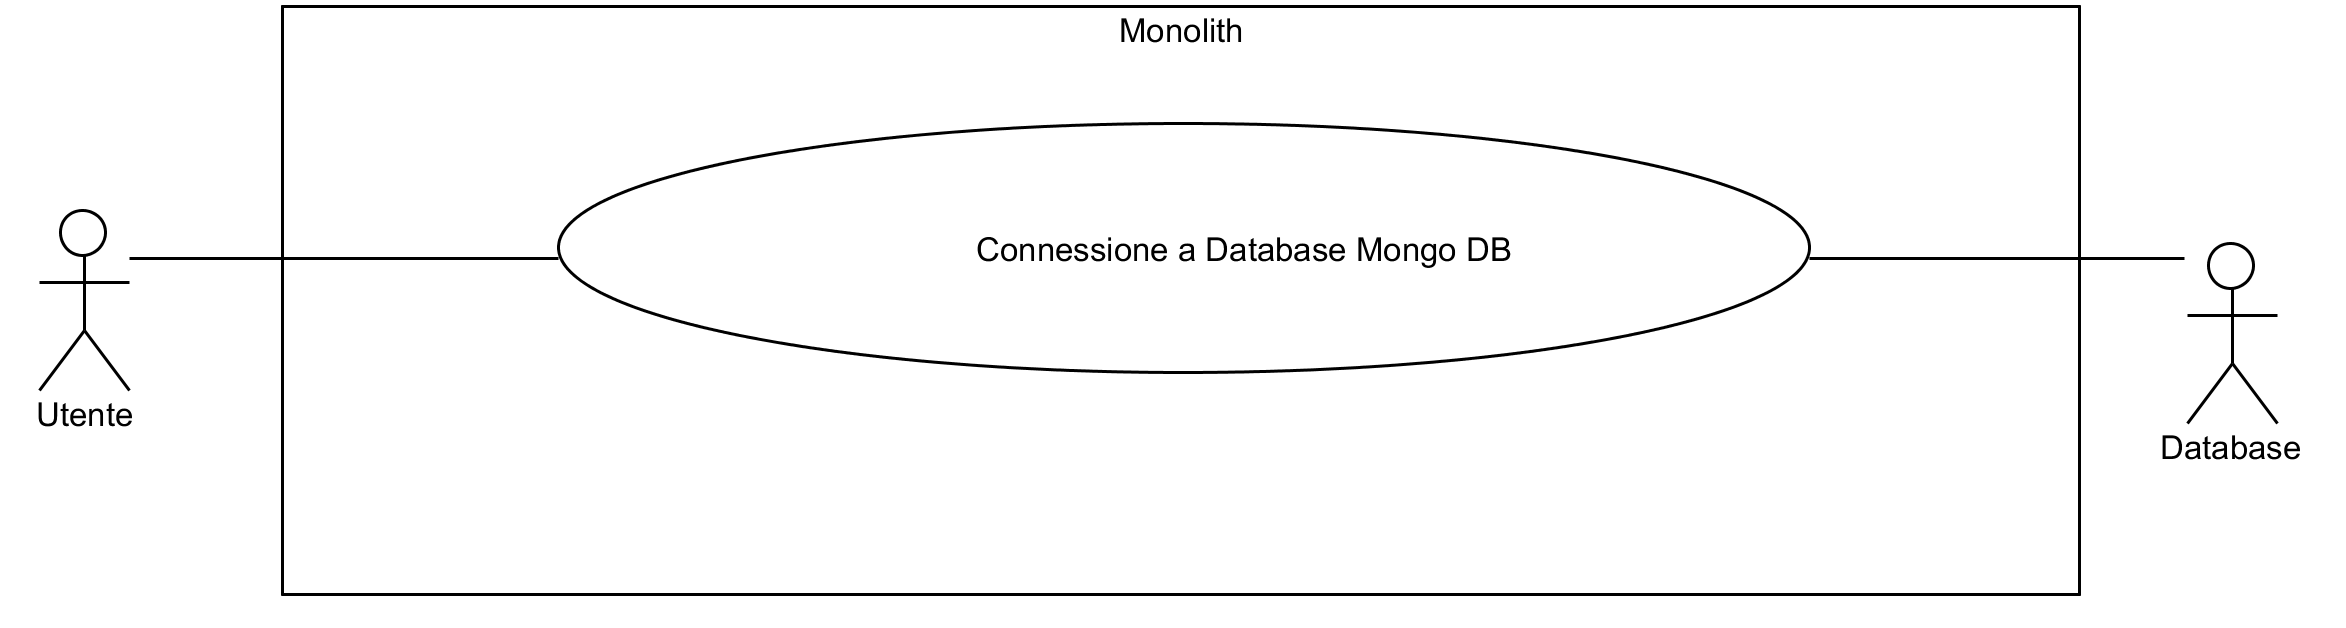
\includegraphics[width=15cm]{../../documenti/AnalisiDeiRequisiti/Diagrammi_img/uc1_00.png}
	\caption{UC1.00 Connessione a database MongoDB}
\end{figure}

\begin{itemize}
\item \textbf{Attori:}
\\Utilizzatore del \glossario{framework}.
\item \textbf{Scopo e descrizione:} 
\\Connettersi ad un database \glossario{MongoDB} esterno all'applicazione.
\item \textbf{Precondizioni:}
	\begin{itemize}
		\item Avere già istanziato una \glossario{bubble generica};
		\item Avere l'indirizzo del database \glossario{MongoDB} a cui si desidera connettersi.
	\end{itemize}
\item \textbf{Flusso principale degli eventi:}
\\L'utilizzatore passa l'indirizzo del database a cui connettersi al metodo che genera una connessione con il database \glossario{MongoDB}.
\item \textbf{Post-condizione:}
\\La \glossario{bubble} generica da cui è invocato il metodo è connessa al database.
\end{itemize}

\subsubsection{UC1.01 Lettura da database MongoDB} \label{UC1.01}

\begin{figure}[H]
	\centering
	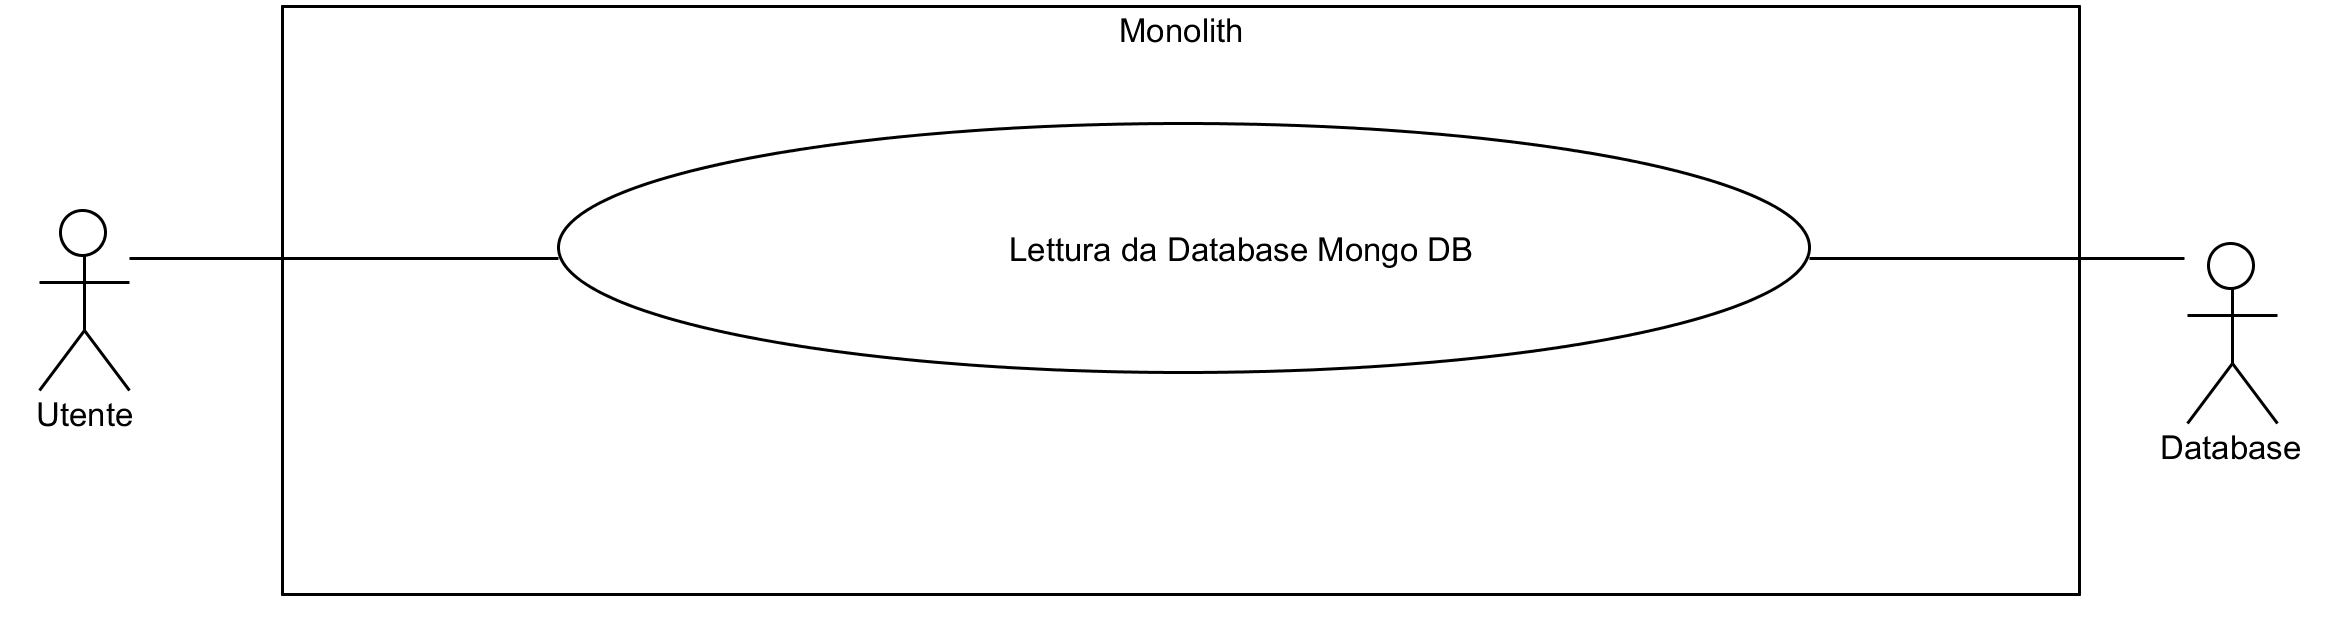
\includegraphics[width=15cm]{../../documenti/AnalisiDeiRequisiti/Diagrammi_img/uc1_01.png}
	\caption{UC1.01 Lettura da database MongoDB}
\end{figure}

\begin{itemize}
	\item \textbf{Attori:}
	\\Utilizzatore del \glossario{framework}.
	\item \textbf{Scopo e descrizione:} 
	\\Prelevare dati dal database connesso alla \glossario{bubble}.
	\item \textbf{Precondizioni:}
	\begin{itemize}
		\item Avere già istanziato una \glossario{bubble generica};
		\item La \glossario{bubble} è connessa al database \glossario{MongoDB} \hyperref[UC1.00]{(UC1.00)};
		\item L'utilizzatore deve conoscere il nome della \glossario{collection} da cui prelevare i dati.
	\end{itemize}
	\item \textbf{Flusso principale degli eventi:}
	\\L'utilizzatore chiama il metodo su una \glossario{bubble}, il quale gli ritorna un oggetto \glossario{JSON} letto dal database, eventualmente assegnabile ad un campo della \glossario{bubble memory}.
	\item \textbf{Post-condizione:}
	\\I dati sono prelevati dal database e sono pronti all'uso nella \glossario{bubble}.
\end{itemize}

\subsubsection{UC1.02 Scrittura su database MongoDB} \label{UC1.02}

\begin{figure}[H]
	\centering
	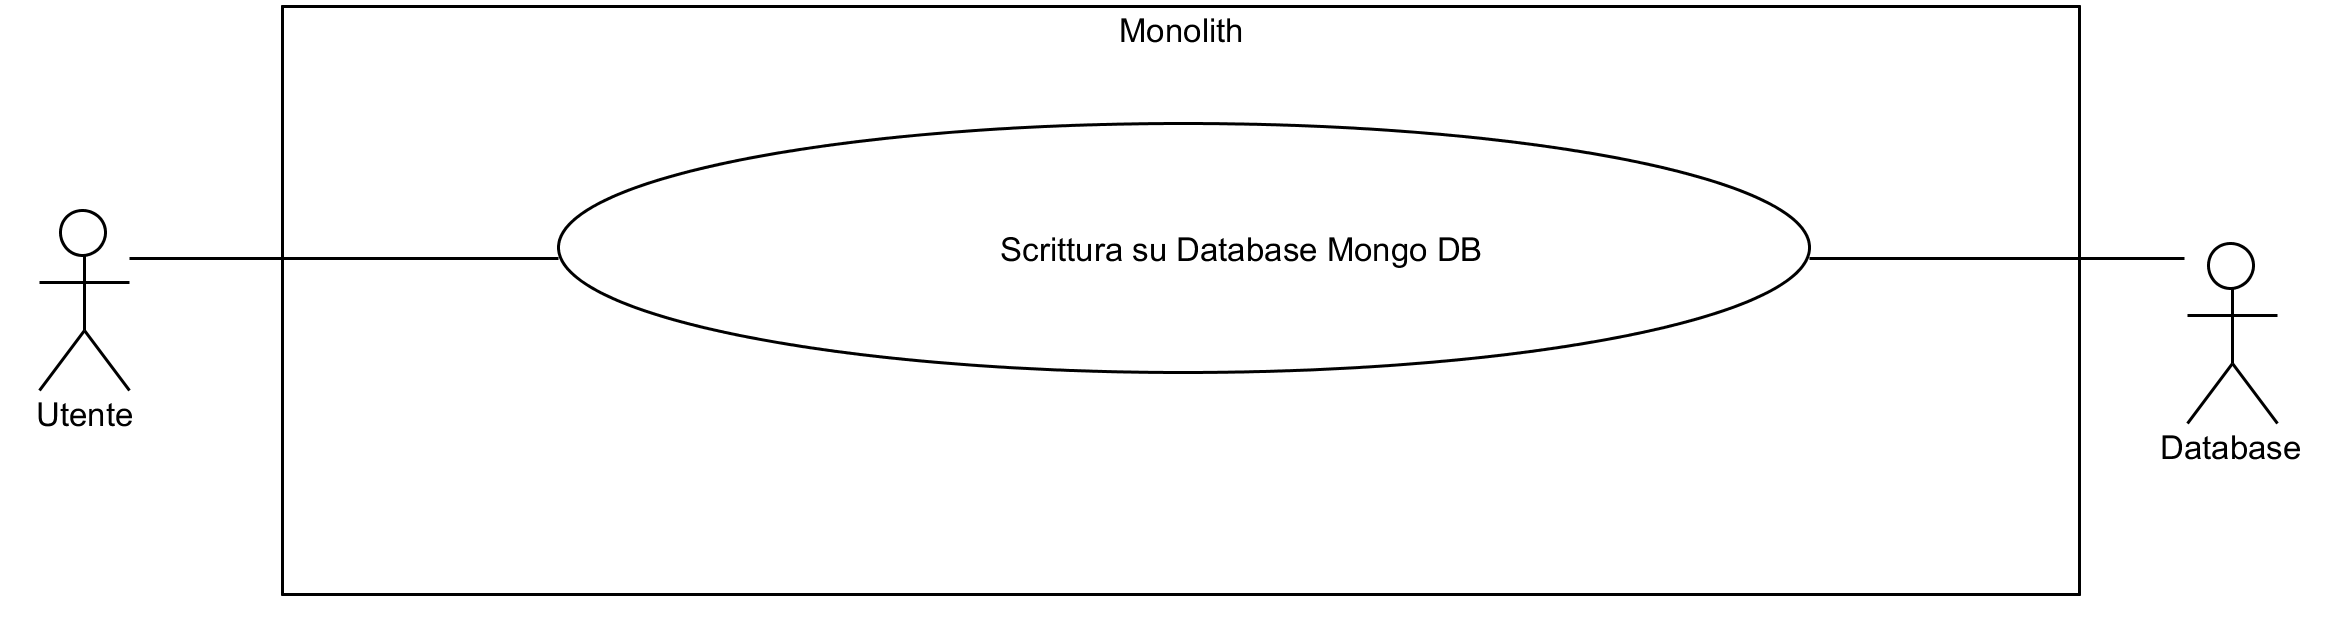
\includegraphics[width=15cm]{../../documenti/AnalisiDeiRequisiti/Diagrammi_img/uc1_02.png}
	\caption{UC1.02 Scrittura su database MongoDB}
\end{figure}

\begin{itemize}
\item \textbf{Attori:}
\\Utilizzatore del \glossario{framework}.
\item \textbf{Scopo e descrizione:} 
\\Scrittura dati nel database connesso alla \glossario{bubble}.
\item \textbf{Precondizioni:}
\begin{itemize}
	\item Avere già istanziato una \glossario{bubble generica};
	\item La \glossario{bubble} è connessa al database \glossario{MongoDB};
	\item L'utilizzatore deve conoscere il nome della \glossario{collection} da cui prelevare i dati.
\end{itemize}
\item \textbf{Flusso principale degli eventi:}
\\L'utilizzatore chiama il metodo su una \glossario{bubble} passandogli un oggetto \glossario{JavaScript}, serializzabile in \glossario{JSON}, e il metodo lo salva nel database.
\item \textbf{Post-condizione:}
\\I dati sono scritti nel database collegato.
\end{itemize}

\subsubsection{UC1.03.1 Rimozione di un elemento} \label{UC1.03.1}

\begin{figure}[H]
	\centering
	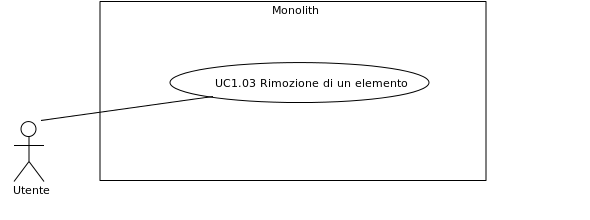
\includegraphics[width=15cm]{../../documenti/AnalisiDeiRequisiti/Diagrammi_img/uc1_03.png}
	\caption{UC1.03.1 Rimozione di un elemento}
\end{figure}

\begin{itemize}
	\item \textbf{Attori:}
	\\Utilizzatore del \glossario{framework}.
	\item \textbf{Scopo e descrizione:} 
	\\Rimuovere dalla \glossario{bubble} un \glossario{elemento} specificato.
	\item \textbf{Precondizioni:}
	\begin{itemize}
		\item Avere già istanziato una \glossario{bubble generica};
		\item La \glossario{bubble} possiede degli elementi.
	\end{itemize}
	\item \textbf{Flusso principale degli eventi:}
	\\L'utilizzatore chiama il metodo, il quale rimuove l'\glossario{elemento} dalla \glossario{bubble}.
	\item \textbf{Scenari alternativi:}
	\\L'elemento non è presente nella \glossario{bubble} \hyperref[UC1.03.2]{(UC1.03.2)}.
	\item \textbf{Post-condizione:}
	\\La \glossario{bubble} non contiene l'elemento indicato da rimuovere.
\end{itemize}

\subsubsection{UC1.03.2 Rimozione di un elemento} \label{UC1.03.2}

\begin{itemize}
	\item \textbf{Attori:}
	\\Utilizzatore del \glossario{framework}.
	\item \textbf{Scopo e descrizione:} 
	\\Rimuovere dalla \glossario{bubble} un \glossario{elemento} specificato.
	\item \textbf{Precondizioni:}
	\begin{itemize}
		\item Avere già istanziato una \glossario{bubble generica};
		\item La \glossario{bubble} possiede degli \glossario{elementi}.
	\end{itemize}
	\item \textbf{Flusso principale degli eventi:}
	\\L'utilizzatore chiama il metodo, il quale, non trovando l'\glossario{elemento}, restituisce un messaggio di errore.
	\item \textbf{Scenari alternativi:}
	\\L'elemento è presente nella \glossario{bubble} \hyperref[UC1.03.1]{(UC1.03.1)}.
	\item \textbf{Post-condizione:}
	\\La \glossario{bubble} non contiene l'elemento indicato da rimuovere e l'utilizzatore è stato avvisato della sua mancanza.
\end{itemize}

\subsubsection{UC1.04 Aggiunta di un elemento} \label{UC1.04}

\begin{figure}[H]
	\centering
	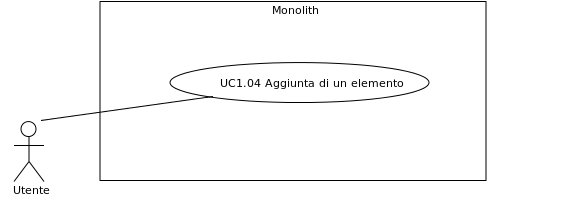
\includegraphics[width=15cm]{../../documenti/AnalisiDeiRequisiti/Diagrammi_img/uc1_04.png}
	\caption{UC1.04 Aggiunta di un elemento}
\end{figure}

\begin{itemize}
	\item \textbf{Attori:}
	\\Utilizzatore del \glossario{framework}.
	\item \textbf{Scopo e descrizione:} 
	\\Inserire nella \glossario{bubble} un \glossario{elemento}.
	\item \textbf{Precondizioni:}
	\begin{itemize}
		\item Avere già istanziato una \glossario{bubble generica};
		\item Aver istanziato un elemento.
	\end{itemize}
	\item \textbf{Flusso principale degli eventi:}
	\\L'utilizzatore invoca il metodo sulla \glossario{bubble} e il metodo lo aggiunge alla \glossario{bubble}.
	\item \textbf{Post-condizione:}
	\\La \glossario{bubble} avrà al suo interno l'\glossario{elemento} passato al metodo.
\end{itemize}

\subsubsection{UC1.05.1 Modifica di un elemento} \label{UC1.05.1}

\begin{figure}[H]
	\centering
	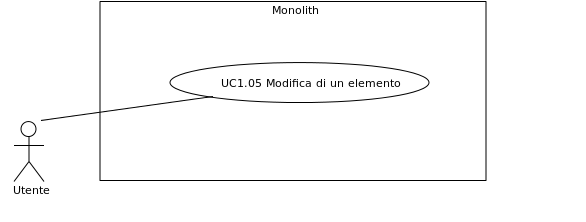
\includegraphics[width=15cm]{../../documenti/AnalisiDeiRequisiti/Diagrammi_img/uc1_05.png}
	\caption{UC1.05.1 Modifica di un elemento}
\end{figure}

\begin{itemize}
	\item \textbf{Attori:}
	\\Utilizzatore del \glossario{framework}.
	\item \textbf{Scopo e descrizione:} 
	\\Modificare un \glossario{elemento} di una \glossario{bubble}.
	\item \textbf{Precondizioni:}
	\begin{itemize}
		\item Avere già istanziato una \glossario{bubble generica};
		\item All'interno della \glossario{bubble} sono presenti degli elementi.
	\end{itemize}
	\item \textbf{Flusso principale degli eventi:}
	\\L'utilizzatore invoca il metodo sulla \glossario{bubble} e il metodo modifica l'\glossario{elemento}.
	\item \textbf{Scenari alternativi:}
	\\L'elemento non è presente nella \glossario{bubble} \hyperref[UC1.05.2]{(UC1.05.2)}.
	\item \textbf{Post-condizione:}
	\\La \glossario{bubble} contiene l'\glossario{elemento} modificato.
\end{itemize}

\subsubsection{UC1.05.2 Modifica di un elemento} \label{UC1.05.2}

\begin{itemize}
	\item \textbf{Attori:}
	\\Utilizzatore del \glossario{framework}.
	\item \textbf{Scopo e descrizione:} 
	\\Modificare un \glossario{elemento} di una \glossario{bubble}.
	\item \textbf{Precondizioni:}
	\begin{itemize}
		\item Avere già istanziato una \glossario{bubble generica};
		\item All'interno della \glossario{bubble} sono presenti degli elementi.
	\end{itemize}
	\item \textbf{Flusso principale degli eventi:}
	\\L'utilizzatore invoca il metodo sulla \glossario{bubble} e il metodo, non trovando l'\glossario{elemento} da modificare, lancia un messaggio di errore.
	\item \textbf{Scenari alternativi:}
	\\L'\glossario{elemento} è presente nella \glossario{bubble} \hyperref[UC1.05.1]{(UC1.05.1)}.
	\item \textbf{Post-condizione:}
	\\L'utilizzatore del metodo è a conoscenza che la modifica è fallita in quanto non era presente l'\glossario{elemento} da modificare.
\end{itemize}

\subsubsection{UC1.06.1 Cambiamento di stato della bubble} \label{UC1.06.1}

\begin{figure}[H]
	\centering
	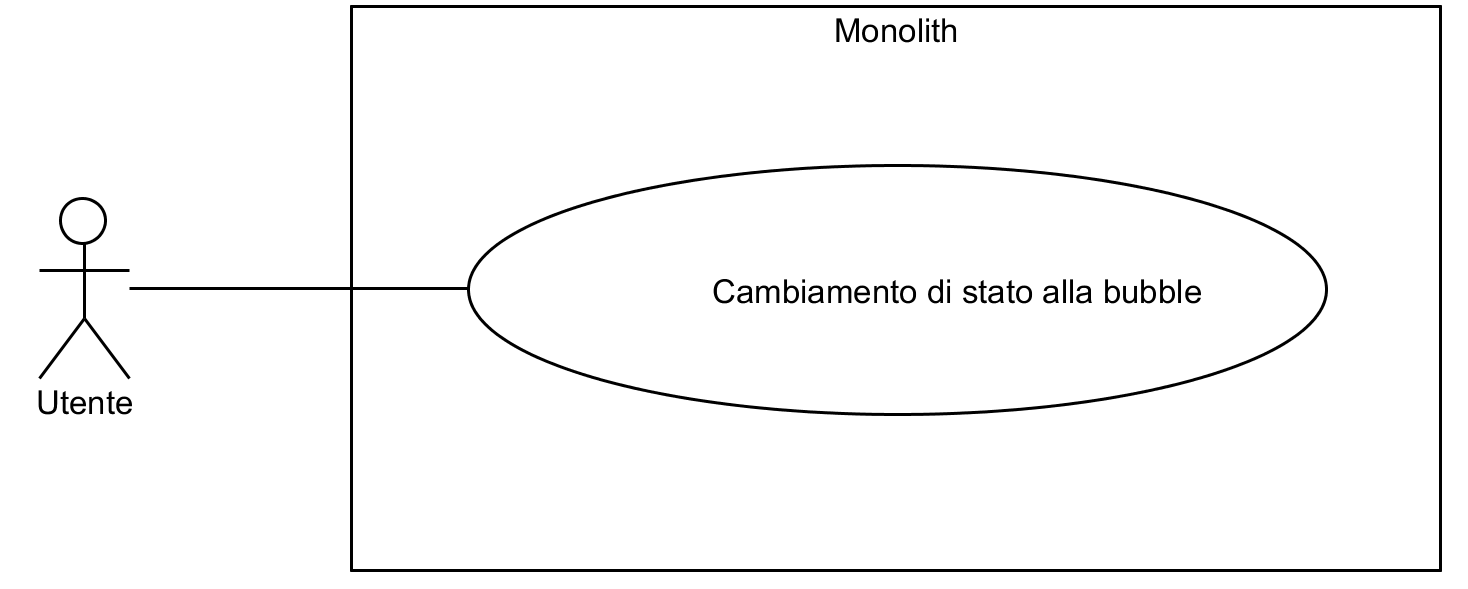
\includegraphics[width=15cm]{../../documenti/AnalisiDeiRequisiti/Diagrammi_img/uc1_06.png}
	\caption{UC1.06.1 Cambiamento di stato della bubble}
\end{figure}

\begin{itemize}
	\item \textbf{Attori:}
	\\Utilizzatore del \glossario{framework}.
	\item \textbf{Scopo e descrizione:} 
	\\Modificare lo specifico stato della \glossario{bubble}.
	\item \textbf{Precondizioni:}
	\begin{itemize}
		\item Avere già istanziato una \glossario{bubble generica}.
	\end{itemize}
	\item \textbf{Flusso principale degli eventi:}
	\\L'utilizzatore invoca il metodo sulla \glossario{bubble} indicando il nuovo stato e il metodo esegue la modifica.
	\item \textbf{Scenari alternativi:}
	\\L'oggetto che si sta cercando di modificare non ha la proprietà cercata \hyperref[UC1.06.2]{(UC1.06.2)}.
	\item \textbf{Post-condizione:}
	\\L'oggetto è stato modificato.
\end{itemize}

\subsubsection{UC1.06.2 Cambiamento di stato della bubble} \label{UC1.06.2}

\begin{itemize}
	\item \textbf{Attori:}
	\\Utilizzatore del \glossario{framework}.
	\item \textbf{Scopo e descrizione:} 
	\\Modificare lo specifico stato della \glossario{bubble}.
	\item \textbf{Precondizioni:}
	\begin{itemize}
		\item Avere già istanziato una \glossario{bubble generica}.
	\end{itemize}
	\item \textbf{Flusso principale degli eventi:}
	\\L'utilizzatore invoca il metodo sulla \glossario{bubble} indicando il nuovo stato e il metodo, non trovando la proprietà cercata, restituisce un messaggio di errore.
	\item \textbf{Scenari alternativi:}
	\\L'oggetto che si sta cercando di modificare ha la proprietà cercata \hyperref[UC1.06.1]{(UC1.06.1)}.
	\item \textbf{Post-condizione:}
	\\L'oggetto non è stato modificato.
\end{itemize}

\subsubsection{UC1.07.1 Chiamata API esterne} \label{UC1.07.1}

\begin{figure}[H]
	\centering
	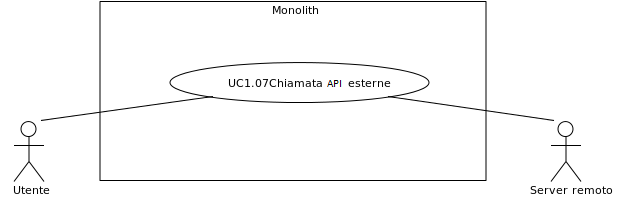
\includegraphics[width=15cm]{../../documenti/AnalisiDeiRequisiti/Diagrammi_img/uc1_07.png}
	\caption{UC1.07.1 Chiamata API esterne}
\end{figure}

\begin{itemize}
	\item \textbf{Attori:}
	\\Utilizzatore del \glossario{framework}.
	\item \textbf{Scopo e descrizione:} 
	\\Ottenere il risultato dell'interrogazione di un servizio esterno al \glossario{framework} tramite chiamata di \glossario{API}.
	\item \textbf{Precondizioni:}
	\begin{itemize}
		\item Avere già istanziato una \glossario{bubble generica};
		\item Conoscere l'URL del servizio desiderato.
	\end{itemize}
	\item \textbf{Flusso principale degli eventi:}
	\\Il metodo prende l'indirizzo del servizio e ritorna in formato \glossario{JSON} il risultato della chiamata.
	\item \textbf{Scenari alternativi:}
	\\Il servizio che si sta cercando di contattare non è disponibile \hyperref[UC1.07.2]{(UC1.07.2)}.
	\item \textbf{Post-condizione:}
	\\All'interno della logica della \glossario{bubble} è utilizzabile il risultato della consultazione del servizio.
\end{itemize}

\subsubsection{UC1.07.2 Chiamata api esterne} \label{UC1.07.2}

\begin{itemize}
	\item \textbf{Attori:}
	\\Utilizzatore del \glossario{framework}.
	\item \textbf{Scopo e descrizione:} 
	\\Ottenere il risultato dell'interrogazione di un servizio esterno al \glossario{framework} tramite chiamata di \glossario{API}.
	\item \textbf{Precondizioni:}
	\begin{itemize}
		\item Avere già istanziato una \glossario{bubble generica};
		\item Conoscere l'URL del servizio desiderato.
	\end{itemize}
	\item \textbf{Flusso principale degli eventi:}
	\\Il metodo prende l'indirizzo del servizio e, non trovandolo disponibile, ritorna un messaggio di errore.
	\item \textbf{Scenari alternativi:}
	\\Il servizio che si sta cercando di contattare è disponibile \hyperref[UC1.07.1]{(UC1.07.1)}.
	\item \textbf{Post-condizione:}
	\\L'utilizzatore del metodo è stato avvisato della non disponibilità del servizio.
\end{itemize}

\subsubsection{UC1.08 Limite interazioni per persona} \label{UC1.08}

\begin{figure}[H]
	\centering
	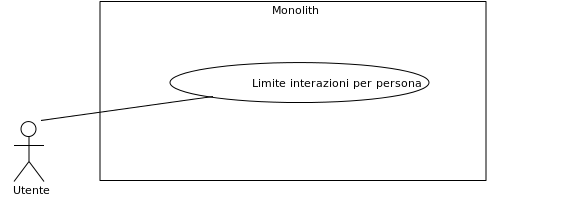
\includegraphics[width=15cm]{../../documenti/AnalisiDeiRequisiti/Diagrammi_img/uc1_08.png}
	\caption{UC1.08 Limite interazioni per persona}
\end{figure}

\begin{itemize}
	\item \textbf{Attori:}
	\\Utilizzatore del \glossario{framework}.
	\item \textbf{Scopo e descrizione:} 
	\\Porre un limite superiore al numero delle interazioni che un utente di \glossario{Rocket.Chat} può avere con una stessa \glossario{bubble}.
	\item \textbf{Precondizioni:}
	\begin{itemize}
		\item Avere già istanziato una \glossario{bubble generica};
		\item Avere almeno un \glossario{elemento di input} all'interno della \glossario{bubble}.
	\end{itemize}
	\item \textbf{Flusso principale degli eventi:}
	\\Alla chiamata del metodo viene specificato il numero massimo di interazioni possibili per una persona con una singola istanza della \glossario{bubble}.
	\item \textbf{Post-condizione:}
	\\Il singolo utilizzatore della \glossario{bubble} come utente di \glossario{Rocket.Chat} non potrà interagire con la stessa istanza della \glossario{bubble} più volte di quelle specificate.
\end{itemize}

\subsubsection{UC1.09 Limite interazioni totali} \label{UC1.09}

\begin{figure}[H]
	\centering
	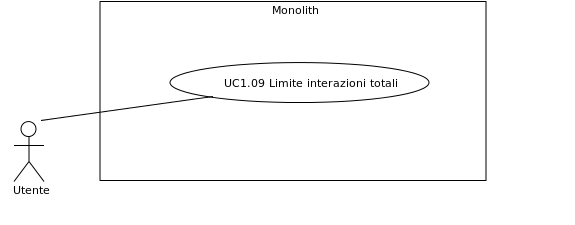
\includegraphics[width=15cm]{../../documenti/AnalisiDeiRequisiti/Diagrammi_img/uc1_09.png}
	\caption{UC1.09 Limite interazioni totali}
\end{figure}

\begin{itemize}
	\item \textbf{Attori:}
	\\Utilizzatore del \glossario{framework}.
	\item \textbf{Scopo e descrizione:} 
	\\Porre un limite superiore al numero delle interazioni che tutti gli utenti possono avere con una stessa istanza della \glossario{bubble}.
	\item \textbf{Precondizioni:}
	\begin{itemize}
		\item Avere già istanziato una \glossario{bubble generica};
		\item Avere almeno un \glossario{elemento} di input all'interno della \glossario{bubble}.
	\end{itemize}
	\item \textbf{Flusso principale degli eventi:}
	\\Alla chiamata del metodo viene specificato il numero massimo di interazioni possibili per l'istanza della \glossario{bubble}.
	\item \textbf{Post-condizione:}
	\\La singola istanza della \glossario{bubble} ha un numero massimo di interazioni possibili condiviso tra tutti i suoi utenti. 
\end{itemize}

\subsubsection{UC1.10 Match con espressione regolare} \label{UC1.10}

\begin{figure}[H]
	\centering
	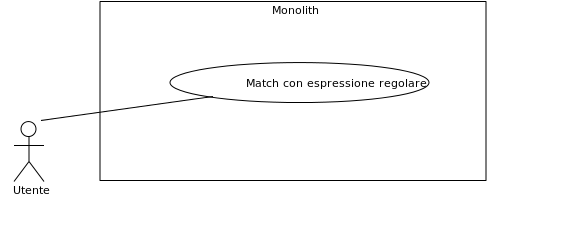
\includegraphics[width=15cm]{../../documenti/AnalisiDeiRequisiti/Diagrammi_img/uc1_10.png}
	\caption{UC1.10 Match con espressione regolare}
\end{figure}

\begin{itemize}
	\item \textbf{Attori:}
	\\Utilizzatore del \glossario{framework}.
	\item \textbf{Scopo e descrizione:} 
	\\Verificare che l'input testuale di una \glossario{bubble} sia compatibile con un'espressione regolare data.
	\item \textbf{Precondizioni:}
	\begin{itemize}
		\item Avere già istanziato una \glossario{bubble generica};
		\item Avere almeno un \glossario{elemento di input} all'interno della \glossario{bubble}.
	\end{itemize}
	\item \textbf{Flusso principale degli eventi:}
	\\Alla chiamata del metodo viene specificato l'\glossario{elemento} da verificare e l'espressione regolare in base a cui controllarlo.
	\item \textbf{Post-condizione:}
	\\È noto se l'input della \glossario{bubble} è corretto secondo l'espressione regolare.
\end{itemize}

\subsubsection{UC1.11 Dimensione massima del file} \label{UC1.11}

\begin{figure}[H]
	\centering
	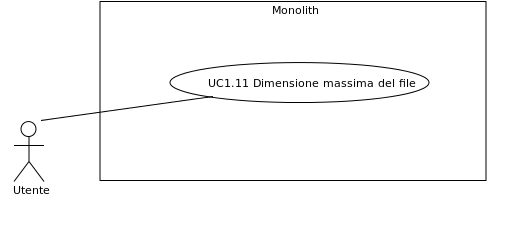
\includegraphics[width=15cm]{../../documenti/AnalisiDeiRequisiti/Diagrammi_img/uc1_11.png}
	\caption{UC1.11 Dimensione massima del file}
\end{figure}

\begin{itemize}
	\item \textbf{Attori:}
	\\Utilizzatore del \glossario{framework}.
	\item \textbf{Scopo e descrizione:} 
	\\Verificare che la dimensione dei file caricati in input sia minore o uguale a quella specificata.
	\item \textbf{Precondizioni:}
	\begin{itemize}
		\item Avere già istanziato una \glossario{bubble generica};
		\item Avere almeno un \glossario{elemento di input} all'interno della \glossario{bubble}.
	\end{itemize}
	\item \textbf{Flusso principale degli eventi:}
	\\Alla chiamata del metodo viene specificata la dimensione massima accettata per i file di input.
	\item \textbf{Post-condizione:}
	\\È stata impostata una dimensione massima per i file allegabili.
\end{itemize}

\subsubsection{UC1.12 Controllo sul JSON} \label{UC1.12}

\begin{figure}[H]
	\centering
	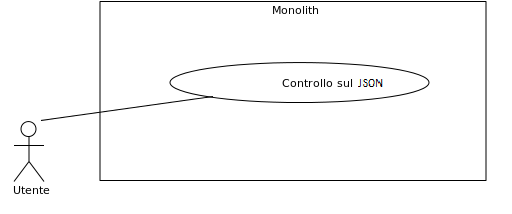
\includegraphics[width=15cm]{../../documenti/AnalisiDeiRequisiti/Diagrammi_img/uc1_12.png}
	\caption{UC1.12 Controllo sul JSON}
\end{figure}

\begin{itemize}
	\item \textbf{Attori:}
	\\Utilizzatore del \glossario{framework}.
	\item \textbf{Scopo e descrizione:} 
	\\Verificare che la struttura di un oggetto \glossario{JSON} sia compatibile con lo schema fornito.
	\item \textbf{Precondizioni:}
	\begin{itemize}
		\item Avere già istanziato una \glossario{bubble generica};
		\item Avere un oggetto \glossario{JSON} da validare;
		\item Avere lo schema attraverso cui validare l'oggetto \glossario{JSON}.
	\end{itemize}
	\item \textbf{Flusso principale degli eventi:}
	\\Alla chiamata del metodo viene specificato il \glossario{JSON} da verificare e lo schema di dati rispetto al quale validare tale oggetto. Il metodo poi si occupa della validazione.
	\item \textbf{Post-condizione:}
	\\È noto se l'oggetto \glossario{JSON} è compatibile con la struttura indicata.
\end{itemize}

\subsubsection{UC1.13 Durata della bubble} \label{UC1.13}

\begin{figure}[H]
	\centering
	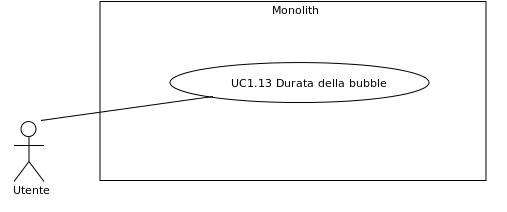
\includegraphics[width=15cm]{../../documenti/AnalisiDeiRequisiti/Diagrammi_img/uc1_13.png}
	\caption{UC1.13 Durata della bubble}
\end{figure}

\begin{itemize}
	\item \textbf{Attori:}
	\\Utilizzatore del \glossario{framework}.
	\item \textbf{Scopo e descrizione:} 
	\\Dare la possibilità all'utilizzatore del \glossario{framework} di impostare un limite temporale entro il quale la \glossario{bubble} smetterà di essere attiva.
	\item \textbf{Precondizioni:}
	\begin{itemize}
		\item Avere già istanziato una \glossario{bubble generica}.
	\end{itemize}
	\item \textbf{Flusso principale degli eventi:}
	\\Alla chiamata del metodo viene specificato il tempo per il quale la \glossario{bubble} sarà attiva.
	\item \textbf{Post-condizione:}
	\\Al termine del periodo di tempo specificato dal metodo verrà invocata la sua terminazione secondo quanto specificato nel caso d'uso \hyperref[UC1.19]{UC1.19} termina \glossario{bubble}.
\end{itemize}

\subsubsection{UC1.14 Lista utenti partecipanti} \label{UC1.14}

\begin{figure}[H]
	\centering
	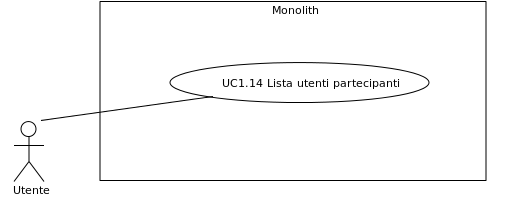
\includegraphics[width=15cm]{../../documenti/AnalisiDeiRequisiti/Diagrammi_img/uc1_14.png}
	\caption{UC1.14 Lista utenti partecipanti}
\end{figure}

\begin{itemize}
	\item \textbf{Attori:}
	\\Utilizzatore del \glossario{framework}.
	\item \textbf{Scopo e descrizione:} 
	\\Possibilità di visualizzare gli utilizzatori correnti della \glossario{bubble}.
	\item \textbf{Precondizioni:}
	\begin{itemize}
		\item Avere già istanziato una \glossario{bubble generica}.
	\end{itemize}
	\item \textbf{Flusso principale degli eventi:}
	\\Alla chiamata del metodo viene specificato l'elenco degli utilizzatori correnti della \glossario{bubble}.
	\item \textbf{Post-condizione:}
	\\Viene restituita una lista di utilizzatori della \glossario{bubble}.
\end{itemize}

\subsubsection{UC1.15.1 Storico interazioni con la bubble per utente} \label{UC1.15.1}

\begin{figure}[H]
	\centering
	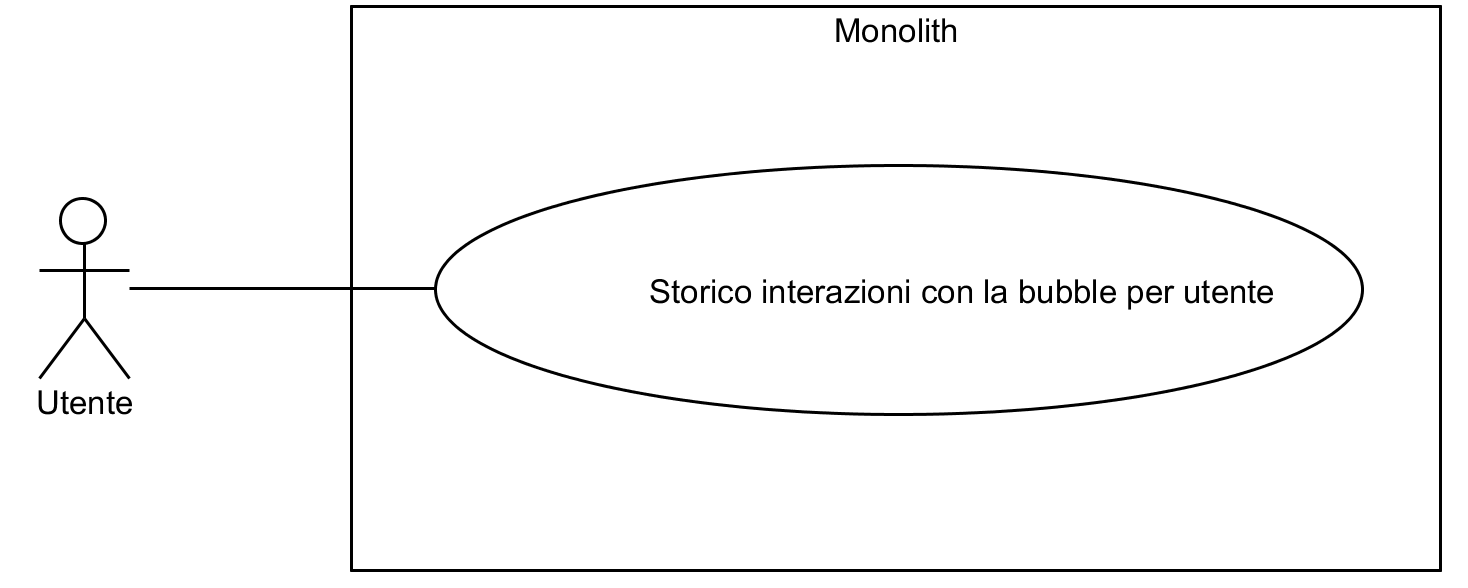
\includegraphics[width=15cm]{../../documenti/AnalisiDeiRequisiti/Diagrammi_img/uc1_15.png}
	\caption{UC1.15.1 Storico interazioni con la bubble per utente}
\end{figure}

\begin{itemize}
	\item \textbf{Attori:}
	\\Utilizzatore del \glossario{framework}.
	\item \textbf{Scopo e descrizione:} 
	\\Dare la possibilità all'utilizzatore del \glossario{framework} di consultare lo storico delle interazioni che un singolo utente ha avuto con la \glossario{bubble}.
	\item \textbf{Precondizioni:}
	\begin{itemize}
		\item Avere già istanziato una \glossario{bubble generica};
		\item Avere elementi di input all'interno della \glossario{bubble}.
	\end{itemize}
	\item \textbf{Flusso principale degli eventi:}
	\\Alla chiamata del metodo viene specificato l'utente di cui si è interessati a conoscere lo storico delle interazioni.
	\item \textbf{Scenari alternativi:}
	\\Non è presente l'utente specificato all'interno della conversazione \hyperref[UC1.15.2]{(UC1.15.2)}.
	\item \textbf{Post-condizione:}
	\\L'informazione relativa allo storico delle interazioni di un singolo utente con la \glossario{bubble} è noto all'interno della \glossario{bubble} stessa.
\end{itemize}

\subsubsection{UC1.15.2 Storico interazioni con la bubble per utente} \label{UC1.15.2}

\begin{itemize}
	\item \textbf{Attori:}
	\\Utilizzatore del \glossario{framework}.
	\item \textbf{Scopo e descrizione:} 
	\\Dare la possibilità all'utilizzatore del \glossario{framework} di consultare lo storico delle interazioni che un singolo utente ha avuto con la \glossario{bubble}.
	\item \textbf{Precondizioni:}
	\begin{itemize}
		\item Avere già istanziato una \glossario{bubble generica};
		\item Avere elementi di input all'interno della \glossario{bubble}.
	\end{itemize}
	\item \textbf{Flusso principale degli eventi:}
	\\Alla chiamata del metodo viene specificato l'utente di cui si è interessati a conoscere lo storico delle interazioni e il metodo, non trovando l'utente, restituisce un messaggio di errore.
	\item \textbf{Scenari alternativi:}
	\\È presente l'utente specificato all'interno della conversazione \hyperref[UC1.15.1]{(UC1.15.1)}.
	\item \textbf{Post-condizione:}
	\\L'utilizzatore del metodo ha ricevuto un messaggio di errore che lo avvisa dell'assenza all'interno della conversazione dell'utente di cui aveva richiesto lo storico.
\end{itemize}

\subsubsection{UC1.16 Esecuzione in orario specificato} \label{UC1.16}

\begin{figure}[H]
	\centering
	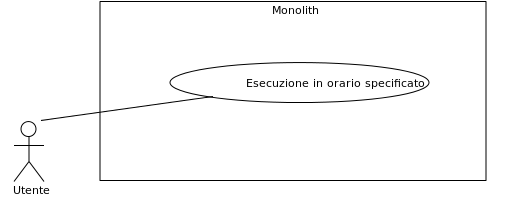
\includegraphics[width=15cm]{../../documenti/AnalisiDeiRequisiti/Diagrammi_img/uc1_16.png}
	\caption{UC1.16 Esecuzione in orario specificato}
\end{figure}

\begin{itemize}
	\item \textbf{Attori:}
	\\Utilizzatore del \glossario{framework}.
	\item \textbf{Scopo e descrizione:} 
	\\L'utilizzatore del \glossario{framework} può fornire un orario per l'esecuzione della funzionalità della \glossario{bubble}.
	\item \textbf{Precondizioni:}
	\begin{itemize}
		\item Avere già istanziato una \glossario{bubble generica};
		\item Avere la funzione di \glossario{callback} che si desidera eseguire all'orario specificato.
	\end{itemize}
	\item \textbf{Flusso principale degli eventi:}
	\\Alla chiamata del metodo viene specificato l'orario di esecuzione della specifica funzionalità della \glossario{bubble}.
	\item \textbf{Post-condizione:}
	\\Nell'orario stabilito viene eseguita la funzionalità della \glossario{bubble}.
\end{itemize}

\subsubsection{UC1.17 Creazione notifica statica} \label{UC1.17}

\begin{figure}[H]
	\centering
	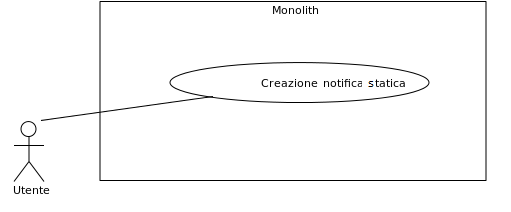
\includegraphics[width=15cm]{../../documenti/AnalisiDeiRequisiti/Diagrammi_img/uc1_17.png}
	\caption{UC1.17 Creazione notifica statica}
\end{figure}

\begin{itemize}
	\item \textbf{Attori:}
	\\Utilizzatore del \glossario{framework}.
	\item \textbf{Scopo e descrizione:} 
	\\L'utilizzatore del \glossario{framework} potrà creare una notifica statica specificandone il testo.
	\item \textbf{Precondizioni:}
	\begin{itemize}
		\item Avere già istanziato una \glossario{bubble generica};
		\item Essere in possesso del messaggio che si desidera notificare sotto forma di testo.
	\end{itemize}
	\item \textbf{Flusso principale degli eventi:}
	\\L'utilizzatore del \glossario{framework} chiama il metodo specificando il testo da visualizzare nella notifica statica.
	\item \textbf{Post-condizione:}
	\\Sul dispositivo sul quale si sta utilizzando \glossario{Rocket.Chat} sarà notificato il testo specificato nel metodo.
\end{itemize}

\subsubsection{UC1.18 Visualizza notifica statica} \label{UC1.18}

\begin{figure}[H]
	\centering
	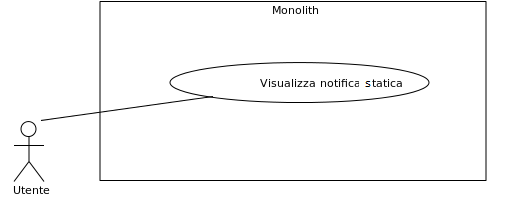
\includegraphics[width=15cm]{../../documenti/AnalisiDeiRequisiti/Diagrammi_img/uc1_18.png}
	\caption{UC1.18 Visualizza notifica statica}
\end{figure}

\begin{itemize}
	\item \textbf{Attori:}
	\\Utilizzatore del \glossario{framework}.
	\item \textbf{Scopo e descrizione:} 
	\\L'utilizzatore del \glossario{framework} può far visualizzare all'utente una notifica statica che visualizzi del testo.
	\item \textbf{Precondizioni:}
	\begin{itemize}
		\item Avere già istanziato una \glossario{bubble generica};
		\item Aver creato una notifica statica.
	\end{itemize}
	\item \textbf{Flusso principale degli eventi:}
	\\L'utilizzatore del \glossario{framework} fa visualizzare una certa notifica da lui creata.
	\item \textbf{Post-condizione:}
	\\La notifica contiene il valore del testo specificato.
\end{itemize}

\subsubsection{UC1.19 Termina bubble} \label{UC1.19}

\begin{figure}[H]
	\centering
	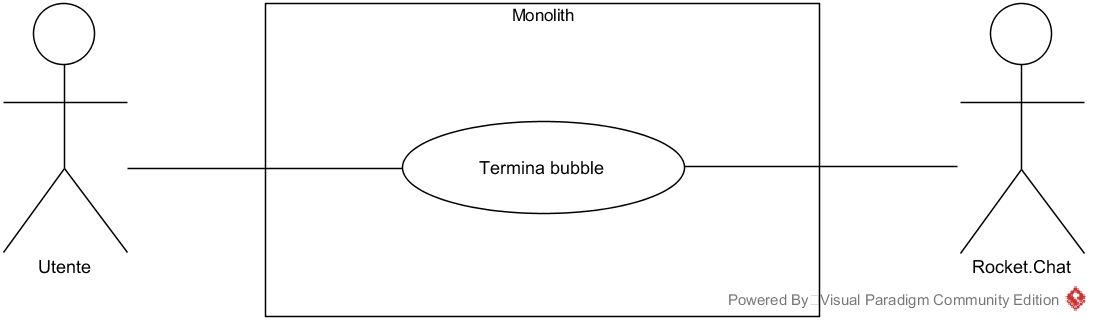
\includegraphics[width=15cm]{../../documenti/AnalisiDeiRequisiti/Diagrammi_img/uc1_19.png}
	\caption{UC1.19 Termina \glossario{bubble}}
\end{figure}

\begin{itemize}
	\item \textbf{Attori:}
	\\Utilizzatore del \glossario{framework}.
	\item \textbf{Scopo e descrizione:} 
	\\L'utilizzatore del framework potrà terminare la \glossario{bubble}.
	\item \textbf{Precondizioni:}
	\begin{itemize}
		\item Avere già istanziato una \glossario{bubble generica}.
	\end{itemize}
	\item \textbf{Flusso principale degli eventi:}
	\\L'utilizzatore del \glossario{framework} chiama il metodo.
	\item \textbf{Post-condizione:}
	\\La \glossario{bubble} è stata terminata e quindi non sarà più possibile interagire con la stessa. L'interfaccia verrà aggiornata, disabilitando la possibilità di dare input e avere output dinamico ma mantenendo un'istantanea del suo ultimo stato.
\end{itemize}

\subsubsection{UC1.20.1 Converti in PDF} \label{UC1.20.1}

\begin{figure}[H]
	\centering
	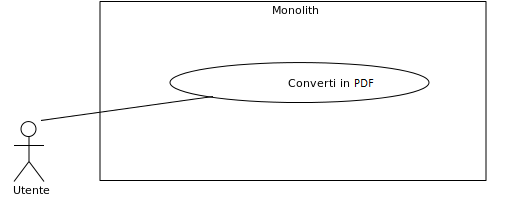
\includegraphics[width=15cm]{../../documenti/AnalisiDeiRequisiti/Diagrammi_img/uc1_20.png}
	\caption{UC1.20.1 Converti in PDF}
\end{figure}

\begin{itemize}
	\item \textbf{Attori:}
	\\Utilizzatore del \glossario{framework}.
	\item \textbf{Scopo e descrizione:} 
	\\L'utilizzatore del \glossario{framework} potrà convertire il testo specificato in un \glossario{PDF}.
	\item \textbf{Precondizioni:}
	\begin{itemize}
		\item Avere già istanziato una \glossario{bubble generica};
		\item Possedere il testo da convertire in formato \glossario{PDF};
		\item Conoscere il percorso in cui si desidera che il file sia salvato.
	\end{itemize}
	\item \textbf{Flusso principale degli eventi:}
	\\L'utilizzatore del \glossario{framework} chiama il metodo specificando il testo da convertire in \glossario{PDF} e il percorso in cui si desidera salvare il file.
	\item \textbf{Scenari alternativi:}
	\\Il salvataggio del file \glossario{PDF} non ha successo \hyperref[UC1.20.2]{(UC1.20.2)}.
	\item \textbf{Post-condizione:}
	\\Un file \glossario{PDF} è stato creato nella posizione corretta e contiene il testo specificato.
\end{itemize}

\subsubsection{UC1.20.2 Conversione in PDF fallita} \label{UC1.20.2}

\begin{itemize}
	\item \textbf{Attori:}
	\\Utilizzatore del \glossario{framework}.
	\item \textbf{Scopo e descrizione:} 
	\\L'utilizzatore del \glossario{framework} potrà convertire il testo specificato in un \glossario{PDF}.
	\item \textbf{Precondizioni:}
	\begin{itemize}
		\item Avere già istanziato una \glossario{bubble generica};
		\item Possedere il testo da convertire in formato \glossario{PDF};
		\item Conoscere il percorso in cui si desidera che il file sia salvato.
	\end{itemize}
	\item \textbf{Flusso principale degli eventi:}
	\\L'utilizzatore del \glossario{framework} chiama il metodo specificando il testo da convertire in \glossario{PDF} e il percorso in cui si desidera salvare il file, ma il salvataggio non avviene e l'utilizzatore del \glossario{framework} visualizza un messaggio d'errore.
	\item \textbf{Scenari alternativi:}
	\\Il salvataggio del file \glossario{PDF} ha successo \hyperref[UC1.20.2]{(UC1.20.2)}.
	\item \textbf{Post-condizione:}
	\\L'utilizzatore del metodo ha ricevuto un messaggio di errore che lo avvisa che il file \glossario{PDF} non è stato salvato.
\end{itemize}

\subsubsection{UC1.21 Mostra elemento grafico} \label{UC1.21}

\begin{figure}[H]
	\centering
	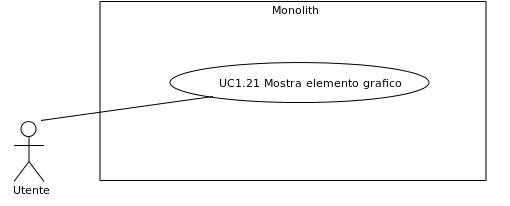
\includegraphics[width=15cm]{../../documenti/AnalisiDeiRequisiti/Diagrammi_img/uc1_21.png}
	\caption{UC1.21 Mostra elemento grafico}
\end{figure}

\begin{itemize}
	\item \textbf{Attori:}
	\\Utilizzatore del \glossario{framework}.
	\item \textbf{Scopo e descrizione:} 
	\\L'utilizzatore del \glossario{framework} potrà mostrare un \glossario{elemento grafico}.
	\item \textbf{Precondizioni:}
	\begin{itemize}
		\item Avere già istanziato una \glossario{bubble generica};
		\item Avere almeno un \glossario{elemento grafico} nella \glossario{bubble}.
	\end{itemize}
	\item \textbf{Flusso principale degli eventi:}
	\\L'utilizzatore del \glossario{framework} chiama il metodo specificando quale \glossario{elemento grafico} della \glossario{bubble} vuole mostrare.
	\item \textbf{Post-condizione:}
	\\L'\glossario{elemento grafico} specificato è visibile.
\end{itemize}

\subsubsection{UC1.22 Nascondi elemento grafico} \label{UC1.22}

\begin{figure}[H]
	\centering
	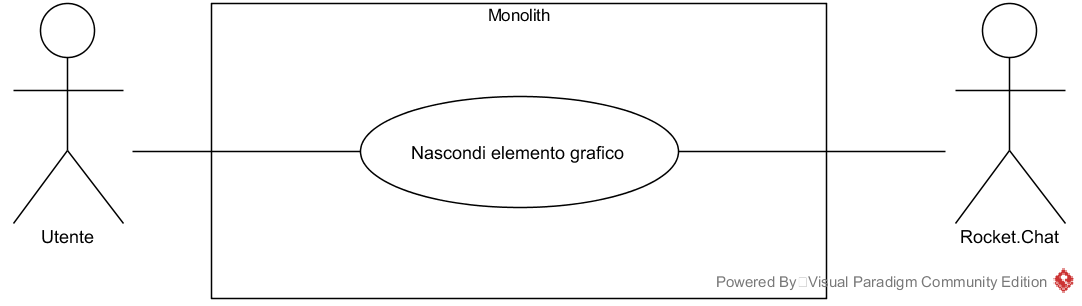
\includegraphics[width=15cm]{../../documenti/AnalisiDeiRequisiti/Diagrammi_img/uc1_22.png}
	\caption{UC1.22 Nascondi elemento grafico}
\end{figure}

\begin{itemize}
	\item \textbf{Attori:}
	\\Utilizzatore del \glossario{framework}.
	\item \textbf{Scopo e descrizione:} 
	\\L'utilizzatore del \glossario{framework} potrà nascondere un \glossario{elemento grafico}.
	\item \textbf{Precondizioni:}
	\begin{itemize}
		\item Avere già istanziato una \glossario{bubble generica};
		\item Avere almeno un \glossario{elemento} nella \glossario{bubble}.
	\end{itemize}
	\item \textbf{Flusso principale degli eventi:}
	\\L'utilizzatore del \glossario{framework} chiama il metodo specificando quale \glossario{elemento grafico} della \glossario{bubble} vuole nascondere.
	\item \textbf{Post-condizione:}
	\\L'\glossario{elemento grafico} specificato non è più visibile.
\end{itemize}

\subsubsection{UC1.23 Imposta posizione elemento grafico} \label{UC1.23}

\begin{figure}[H]
	\centering
	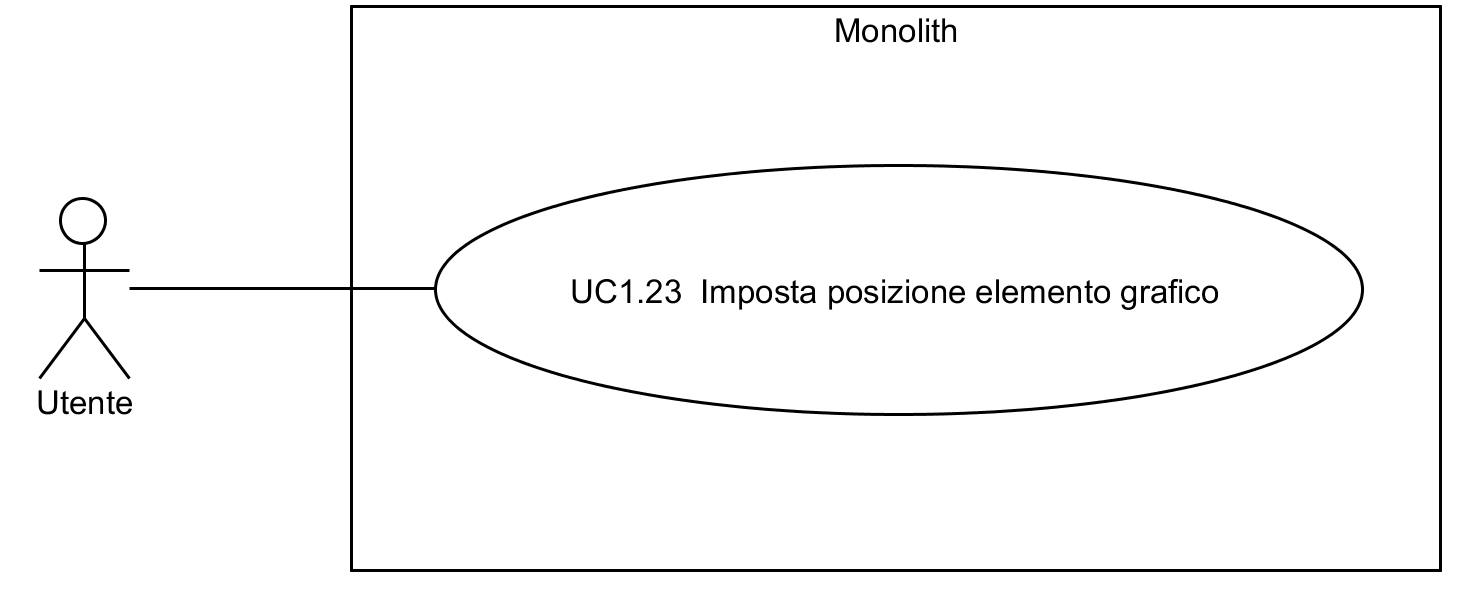
\includegraphics[width=15cm]{../../documenti/AnalisiDeiRequisiti/Diagrammi_img/uc1_23.png}
	\caption{UC1.23 Imposta posizione elemento grafico}
\end{figure}

\begin{itemize}
	\item \textbf{Attori:}
	\\Utilizzatore del \glossario{framework}.
	\item \textbf{Scopo e descrizione:} 
	\\L'utilizzatore del \glossario{framework} può specificare una posizione per un \glossario{elemento grafico} della \glossario{bubble}.
	\item \textbf{Precondizioni:}
	\begin{itemize}
		\item Avere già istanziato una \glossario{bubble generica};
		\item Avere almeno un componente nella \glossario{bubble}.
	\end{itemize}
	\item \textbf{Flusso principale degli eventi:}
	\\L'utilizzatore del \glossario{framework} chiama il metodo specificando la posizione e l'\glossario{elemento grafico} di cui vuole fissare la posizione.
	\item \textbf{Post-condizione:}
	\\L'\glossario{elemento grafico} specificato si trova nella posizione specificata.
\end{itemize}

\subsubsection{UC1.24.1 File output} \label{UC1.24.1}

\begin{figure}[H]
	\centering
	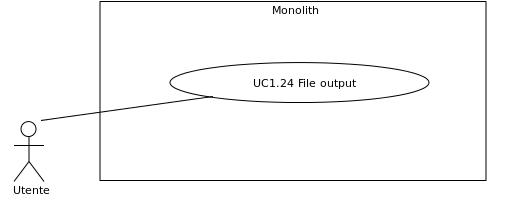
\includegraphics[width=15cm]{../../documenti/AnalisiDeiRequisiti/Diagrammi_img/uc1_24.png}
	\caption{UC1.24.1 File output}
\end{figure}

\begin{itemize}
	\item \textbf{Attori:}
	\\Utilizzatore del \glossario{framework}.
	\item \textbf{Scopo e descrizione:} 
	\\L'utilizzatore del \glossario{framework} può salvare l'output della \glossario{bubble} in un file.
	\item \textbf{Precondizioni:}
	\begin{itemize}
		\item Avere già istanziato una \glossario{bubble generica};
		\item Avere almeno un \glossario{elemento} nella \glossario{bubble}.
	\end{itemize}
	\item \textbf{Flusso principale degli eventi:}
	\\L'utilizzatore del \glossario{framework} chiama il metodo che specifica che l'output della \glossario{bubble} sia un file e le informazioni da salvare in esso.
	\item \textbf{Scenari alternativi:}
	\\Il salvataggio del file non ha successo, in tale caso verrà notificata la condizione anomala con un messaggio d'errore \hyperref[UC1.24.2]{(UC1.24.2)}.
	\item \textbf{Post-condizione:}
	\\Verrà generato un file contenente l'informazione desiderata.
\end{itemize}

\subsubsection{UC1.24.2 Errore File output} \label{UC1.24.2}

\begin{itemize}
	\item \textbf{Attori:}
	\\Utilizzatore del \glossario{framework}.
	\item \textbf{Scopo e descrizione:} 
	\\L'utilizzatore del \glossario{framework} può salvare l'output della \glossario{bubble} in un file, il salvataggio non va a buon fine e viene generato un messaggio d'errore.
	\item \textbf{Precondizioni:}
	\begin{itemize}
		\item Avere già istanziato una \glossario{bubble generica};
		\item Avere delle informazioni da esportare.
	\end{itemize}
	\item \textbf{Flusso principale degli eventi:}
	\\L'utilizzatore del \glossario{framework} chiama il metodo che specifica che l'output della \glossario{bubble} sia un file e le informazioni da salvare in esso, il salvataggio non va a buon fine e viene generato un messaggio d'errore.
	\item \textbf{Scenari alternativi:}
	\\Il salvataggio del file ha successo \hyperref[UC1.24.1]{(UC1.24.1)}.
	\item \textbf{Post-condizione:}
	\\Viene generato un messaggio d'errore.
\end{itemize}

\subsubsection{UC1.25 Immagine} \label{UC1.25}

\begin{figure}[H]
	\centering
	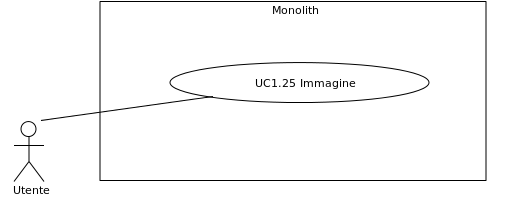
\includegraphics[width=15cm]{../../documenti/AnalisiDeiRequisiti/Diagrammi_img/uc1_25.png}
	\caption{UC1.25 Immagine}
\end{figure}

\begin{itemize}
	\item \textbf{Attori:}
	\\Utilizzatore del \glossario{framework}.
	\item \textbf{Scopo e descrizione:} 
	\\L'utilizzatore del \glossario{framework} può inserire all'interno della \glossario{bubble} un file immagine.
	\item \textbf{Precondizioni:}
	\begin{itemize}
		\item Avere già istanziato una \glossario{bubble generica};
		\item Avere un'immagine di cui fare la preview.
	\end{itemize}
	\item \textbf{Flusso principale degli eventi:}
	\\L'utilizzatore del \glossario{framework} chiama il metodo che specifica il file immagine da includere nella \glossario{bubble}.
	\item \textbf{Post-condizione:}
	\\Il file immagine è stato incluso nella \glossario{bubble}.
\end{itemize}

\subsubsection{UC1.26 TextView} \label{UC1.26}

\begin{figure}[H]
	\centering
	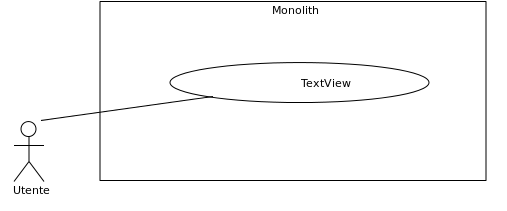
\includegraphics[width=15cm]{../../documenti/AnalisiDeiRequisiti/Diagrammi_img/uc1_26.png}
	\caption{UC1.26 TextView}
\end{figure}

\begin{itemize}
	\item \textbf{Attori:}
	\\Utilizzatore del \glossario{framework}.
	\item \textbf{Scopo e descrizione:} 
	\\L'utilizzatore del \glossario{framework} può inserire all'interno della \glossario{bubble} una \glossario{TextView}.
	\item \textbf{Precondizioni:}
	\begin{itemize}
		\item Avere già istanziato una \glossario{bubble generica};
		\item Avere un testo da visualizzare.
	\end{itemize}
	\item \textbf{Flusso principale degli eventi:}
	\\L'utilizzatore del \glossario{framework} chiama il metodo che specifica il testo da includere nella \glossario{bubble}.
	\item \textbf{Post-condizione:}
	\\Il testo è stato incluso nella \glossario{bubble}.
\end{itemize}

\subsubsection{UC1.27 Label} \label{UC1.27}

\begin{figure}[H]
	\centering
	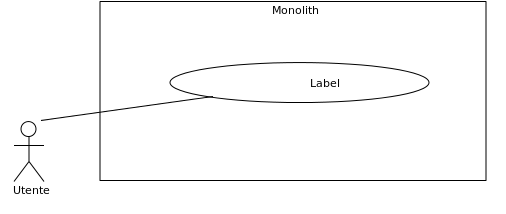
\includegraphics[width=15cm]{../../documenti/AnalisiDeiRequisiti/Diagrammi_img/uc1_27.png}
	\caption{UC1.27 Label}
\end{figure}

\begin{itemize}
	\item \textbf{Attori:}
	\\Utilizzatore del \glossario{framework}.
	\item \textbf{Scopo e descrizione:} 
	\\L'utilizzatore del \glossario{framework} può inserire all'interno della \glossario{bubble} una \glossario{label}.
	\item \textbf{Precondizioni:}
	\begin{itemize}
		\item Avere già istanziato una \glossario{bubble generica};
		\item Avere un testo da visualizzare.
	\end{itemize}
	\item \textbf{Flusso principale degli eventi:}
	\\L'utilizzatore del \glossario{framework} chiama il metodo che specifica il testo da includere nella \glossario{label}.
	\item \textbf{Post-condizione:}
	\\Il testo è stato incluso nella \glossario{bubble}.
\end{itemize}

\subsubsection{UC1.28 Grafico a torta} \label{UC1.28}

\begin{figure}[H]
	\centering
	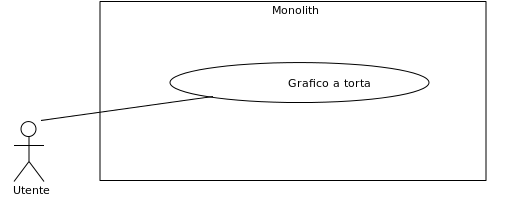
\includegraphics[width=15cm]{../../documenti/AnalisiDeiRequisiti/Diagrammi_img/uc1_28.png}
	\caption{UC1.28 Grafico a torta}
\end{figure}

\begin{itemize}
	\item \textbf{Attori:}
	\\Utilizzatore del \glossario{framework}.
	\item \textbf{Scopo e descrizione:} 
	\\L'utilizzatore del \glossario{framework} può inserire all'interno della \glossario{bubble} un grafico a torta.
	\item \textbf{Precondizioni:}
	\begin{itemize}
		\item Avere già istanziato una \glossario{bubble generica};
		\item Essere in possesso dei dati che si desidera visualizzare nel grafico.
	\end{itemize}
	\item \textbf{Flusso principale degli eventi:}
	\\L'utilizzatore del \glossario{framework} chiama il metodo specificando i dati da rappresentare nel grafico a torta.
	\item \textbf{Post-condizione:}
	\\I dati sono rappresentati nel grafico a torta. Il grafico è visualizzato nella \glossario{bubble}.
\end{itemize}

\subsubsection{UC1.29 Grafico a istogramma} \label{UC1.29}

\begin{figure}[H]
	\centering
	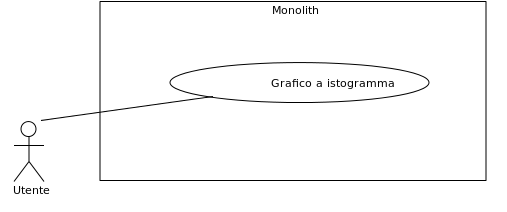
\includegraphics[width=15cm]{../../documenti/AnalisiDeiRequisiti/Diagrammi_img/uc1_29.png}
	\caption{UC1.29 Grafico a istogramma}
\end{figure}

\begin{itemize}
	\item \textbf{Attori:}
	\\Utilizzatore del \glossario{framework}.
	\item \textbf{Scopo e descrizione:} 
	\\L'utilizzatore del \glossario{framework} può inserire all'interno della \glossario{bubble} un grafico istogramma.
	\item \textbf{Precondizioni:}
	\begin{itemize}
		\item Avere già istanziato una \glossario{bubble generica};
		\item Essere in possesso dei dati che si desidera visualizzare nel grafico.
	\end{itemize}
	\item \textbf{Flusso principale degli eventi:}
	\\L'utilizzatore del \glossario{framework} chiama il metodo specificando i dati da rappresentare nel grafico a istogramma.
	\item \textbf{Post-condizione:}
	\\I dati sono rappresentati nel grafico a istogramma. Il grafico è visualizzato nella \glossario{bubble}.
\end{itemize}

\subsubsection{UC1.30 Checkbox} \label{UC1.30}

\begin{figure}[H]
	\centering
	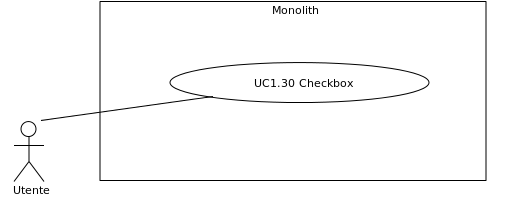
\includegraphics[width=15cm]{../../documenti/AnalisiDeiRequisiti/Diagrammi_img/uc1_30.png}
	\caption{UC1.30 Checkbox}
\end{figure}

\begin{itemize}
	\item \textbf{Attori:}
	\\Utilizzatore del \glossario{framework}.
	\item \textbf{Scopo e descrizione:} 
	\\L'utilizzatore del \glossario{framework} può inserire un \glossario{elemento} \glossario{checkbox} all'interno della \glossario{bubble} specificando la variabile della \glossario{bubble memory} a cui l'\glossario{elemento} è assegnato.
	\item \textbf{Precondizioni:}
	\begin{itemize}
		\item Avere già istanziato una \glossario{bubble generica}.
	\end{itemize}
	\item \textbf{Flusso principale degli eventi:}
	\\L'utilizzatore del \glossario{framework} chiama il metodo per aggiungere alla \glossario{bubble} una \glossario{checkbox} relativa ad un \glossario{elemento} della \glossario{bubble memory} specificato.
	\item \textbf{Post-condizione:}
	\\Nella \glossario{bubble} è presente la \glossario{checkbox}, nella \glossario{bubble memory} è presente la variabile a cui è assegnata.
\end{itemize}

\subsubsection{UC1.31 Bottone Radio} \label{UC1.31}

\begin{figure}[H]
	\centering
	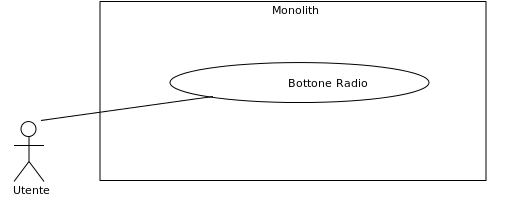
\includegraphics[width=15cm]{../../documenti/AnalisiDeiRequisiti/Diagrammi_img/uc1_31.png}
	\caption{UC1.31 Bottone Radio}
\end{figure}

\begin{itemize}
	\item \textbf{Attori:}
	\\Utilizzatore del \glossario{framework}.
	\item \textbf{Scopo e descrizione:} 
	\\L'utilizzatore del \glossario{framework} può inserire un \glossario{elemento} \glossario{bottone radio} di scelta di un \glossario{elemento} tra molti all'interno della \glossario{bubble}, specificando la variabile della \glossario{bubble memory} a cui la scelta è assegnata.
	\item \textbf{Precondizioni:}
	\begin{itemize}
		\item Avere già istanziato una \glossario{bubble generica}.
	\end{itemize}
	\item \textbf{Flusso principale degli eventi:}
	\\L'utilizzatore del \glossario{framework} chiama il metodo per aggiungere alla \glossario{bubble} un \glossario{bottone radio} relativo ad un \glossario{elemento} della \glossario{bubble memory} specificato.
	\item \textbf{Post-condizione:}
	\\Nella \glossario{bubble} è presente il \glossario{bottone radio}, nella \glossario{bubble memory} è presente la variabile a cui è assegnata.
\end{itemize}

\subsubsection{UC1.32 Bottone} \label{UC1.32}

\begin{figure}[H]
	\centering
	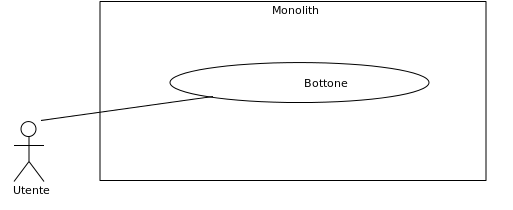
\includegraphics[width=15cm]{../../documenti/AnalisiDeiRequisiti/Diagrammi_img/uc1_32.png}
	\caption{UC1.32 Bottone}
\end{figure}

\begin{itemize}
	\item \textbf{Attori:}
	\\Utilizzatore del \glossario{framework}.
	\item \textbf{Scopo e descrizione:} 
	\\L'utilizzatore del \glossario{framework} può inserire un \glossario{elemento} \glossario{bottone} all'interno della \glossario{bubble} specificando la funzione che verrà eseguita alla pressione del \glossario{bottone} da parte dell'utente.
	\item \textbf{Precondizioni:}
	\begin{itemize}
		\item Avere già istanziato una \glossario{bubble generica};
		\item Avere la funzione da eseguire.
	\end{itemize}
	\item \textbf{Flusso principale degli eventi:}
	\\L'utilizzatore del \glossario{framework} chiama il metodo per aggiungere il \glossario{bottone} specificando la funzione da assegnare ad esso.
	\item \textbf{Post-condizione:}
	\\Nella \glossario{bubble} è presente il \glossario{bottone}. Alla pressione da parte dell'utente del \glossario{bottone} della \glossario{bubble} la funzione di \glossario{callback} specificata verrà eseguita.
\end{itemize}

\subsubsection{UC1.33 TextEdit} \label{UC1.33}

\begin{figure}[H]
	\centering
	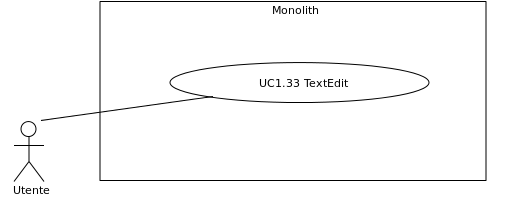
\includegraphics[width=15cm]{../../documenti/AnalisiDeiRequisiti/Diagrammi_img/uc1_33.png}
	\caption{UC1.33 TextEdit}
\end{figure}

\begin{itemize}
	\item \textbf{Attori:}
	\\Utilizzatore del \glossario{framework}.
	\item \textbf{Scopo e descrizione:} 
	\\L'utilizzatore del \glossario{framework} può richiedere un input testuale \glossario{TextEdit}.
	\item \textbf{Precondizioni:}
	\begin{itemize}
		\item Avere già istanziato una \glossario{bubble generica}.
	\end{itemize}
	\item \textbf{Flusso principale degli eventi:}
	\\L'utilizzatore del \glossario{framework} chiama il metodo per aggiungere il testo ricevuto nella \glossario{bubble memory}.
	\item \textbf{Post-condizione:}
	\\Nella \glossario{bubble} è presente il campo di compilazione \glossario{TextEdit}. Nella \glossario{bubble memory} è presente il valore attuale del testo presente nell'\glossario{elemento} della \glossario{bubble}.
\end{itemize}

\subsubsection{UC1.34 File input} \label{UC1.34}

\begin{figure}[H]
	\centering
	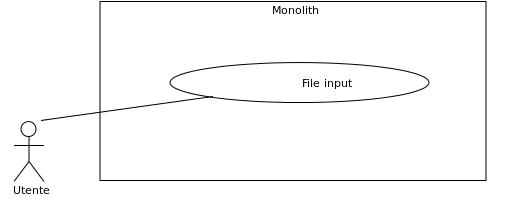
\includegraphics[width=15cm]{../../documenti/AnalisiDeiRequisiti/Diagrammi_img/uc1_34.png}
	\caption{UC1.34 File input}
\end{figure}

\begin{itemize}
	\item \textbf{Attori:}
	\\Utilizzatore del \glossario{framework}.
	\item \textbf{Scopo e descrizione:} 
	\\L'utilizzatore del \glossario{framework} può richiedere l'input di un file.
	\item \textbf{Precondizioni:}
	\begin{itemize}
		\item Avere già istanziato una \glossario{bubble generica}.
	\end{itemize}
	\item \textbf{Flusso principale degli eventi:}
	\\L'utilizzatore del \glossario{framework} chiama il metodo che restituisce il file in input.
	\item \textbf{Post-condizione:}
	\\Il file è stato caricato e passato alla \glossario{bubble}.
\end{itemize}

\subsubsection{UC1.35 Istanziazione della bubble generica} \label{UC1.35}

\begin{figure}[H]
	\centering
	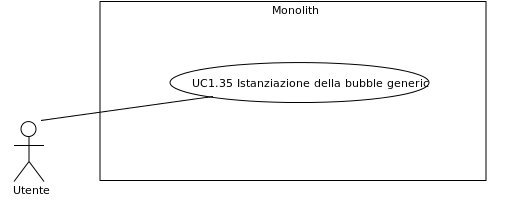
\includegraphics[width=15cm]{../../documenti/AnalisiDeiRequisiti/Diagrammi_img/uc1_35.png}
	\caption{UC1.35 Istanziazione della bubble generica}
\end{figure}

\begin{itemize}
	\item \textbf{Attori:}
	\\Utilizzatore del \glossario{framework}.
	\item \textbf{Scopo e descrizione:} 
	\\L'utilizzatore del \glossario{framework} può istanziare il contenitore \glossario{bubble generica}, il quale funge da contenitore dei vari elementi di input, output e di logica specificati all'interno del \glossario{framework}.
	\item \textbf{Flusso principale degli eventi:}
	\\L'utilizzatore del \glossario{framework} chiama il metodo per istanziare la \glossario{bubble generica} e la memoria ad essa associata.
	\item \textbf{Post-condizione:}
	\\È presente la \glossario{bubble generica}, compresa la sua memoria.
\end{itemize}

\subsubsection{UC1.36 Mostrare bubble generica} \label{UC1.36}

\begin{figure}[H]
	\centering
	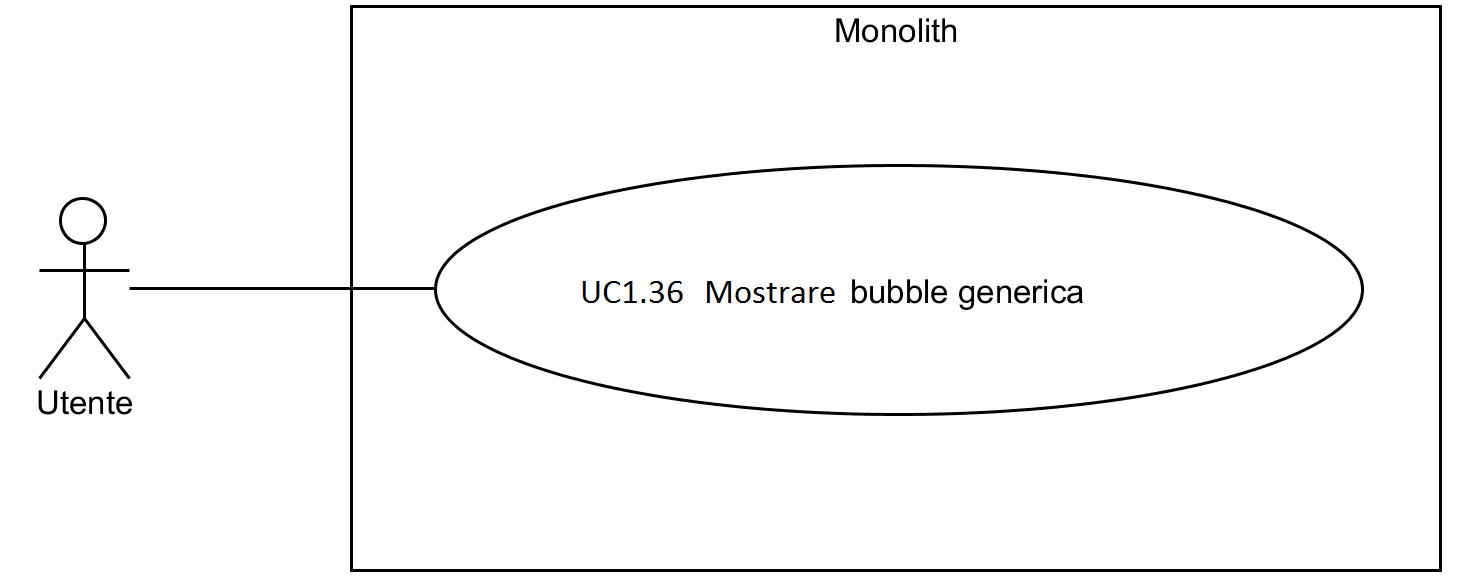
\includegraphics[width=15cm]{../../documenti/AnalisiDeiRequisiti/Diagrammi_img/uc1_36.png}
	\caption{UC1.36 Mostrare bubble generica}
\end{figure}

\begin{itemize}
	\item \textbf{Attori:}
	\\Utilizzatore del \glossario{framework}.
	\item \textbf{Scopo e descrizione:} 
	\\L'utilizzatore del \glossario{framework}, utilizzando questo metodo, rende la \glossario{bubble} visibile all'interno della chat.
	\item \textbf{Precondizioni:}
	\begin{itemize}
		\item Avere già istanziato una \glossario{bubble generica}.
	\end{itemize}
	\item \textbf{Flusso principale degli eventi:}
	\\L'utilizzatore del \glossario{framework} chiama il metodo.
	\item \textbf{Post-condizione:}
	\\La \glossario{bubble} specificata viene mostrata all'interno della chat.
\end{itemize}

\subsection{To-do list}

\subsubsection{UC2.1 Creare una lista} \label{UC2.1}

\begin{figure}[H]
	\centering
	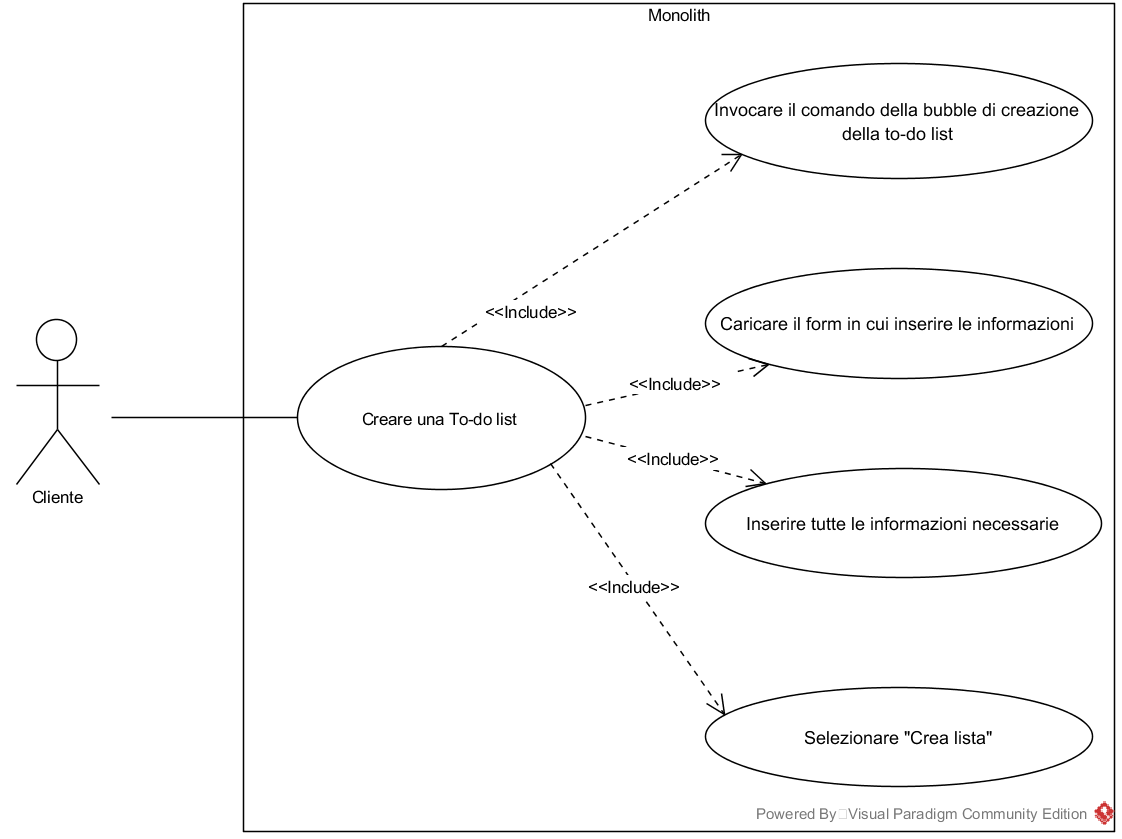
\includegraphics[width=15cm]{../../documenti/AnalisiDeiRequisiti/Diagrammi_img/uc2_1.png}
	\caption{UC2.1 Creare una lista}
\end{figure}

\begin{itemize}
	\item \textbf{Attori:}
	\\Utente di \glossario{Rocket.Chat} in possesso di \ProjectName{}.
	\item \textbf{Scopo e descrizione:} 
	\\Creare una lista di cose da fare.
	\item \textbf{Precondizioni:}
	\begin{itemize}
		\item Essere utenti di \glossario{Rocket.Chat};
		\item Avere \ProjectName installato.
	\end{itemize}
	\item \textbf{Flusso principale degli eventi:}
	\begin{itemize}
		\item L'utente invoca il comando di creazione della \glossario{bubble} \glossario{To-do list} \hyperref[UC2.1.1]{(UC2.1.1)};
		\item L'utente carica il form in cui inserire le informazioni \hyperref[UC2.1.2]{(UC2.1.2)};
		\item L'utente inserisce tutte le informazioni necessarie \hyperref[UC2.1.3]{(UC2.1.3)};
		\item L'utente seleziona \virgolette{Crea lista} \hyperref[UC2.1.4]{(UC2.1.4)}.
	\end{itemize}
	\item \textbf{Post-condizione:}
	\\Nella conversazione è presente una \glossario{bubble} \glossario{To-do list} con il titolo indicato.
\end{itemize}

\subsubsection{UC2.1.1 Invocare il comando della bubble di creazione della to-do list} \label{UC2.1.1}

\begin{itemize}
	\item \textbf{Attori:}
	\\Utente di \glossario{Rocket.Chat} in possesso di \ProjectName{}.
	\item \textbf{Scopo e descrizione:} 
	\\Creare una \glossario{to-do list} all'interno della chat.
	\item \textbf{Precondizioni:}
	\begin{itemize}
		\item Essere utenti di \glossario{Rocket.Chat};
		\item Avere \ProjectName{} installato;
		\item Avere accesso alla \glossario{bubble} \glossario{To-do list}.
	\end{itemize}
	\item \textbf{Flusso principale degli eventi:}
	\\L'utilizzatore di \ProjectName{} utilizzando l'apposito comando inizia la creazione della \glossario{bubble} \glossario{To-do list}.
	\item \textbf{Post-condizione:}
	\\Viene istanziata la \glossario{bubble}.
\end{itemize}

\subsubsection{UC2.1.2 Caricare il form in cui inserire le informazioni} \label{UC2.1.2}

\begin{itemize}
	\item \textbf{Attori:}
	\\Utente di \glossario{Rocket.Chat} in possesso di \ProjectName{}.
	\item \textbf{Scopo e descrizione:} 
	\\Creare una \glossario{to-do list} all'interno della chat.
	\item \textbf{Precondizioni:}
	\begin{itemize}
		\item Essere utenti di \glossario{Rocket.Chat};
		\item Avere \ProjectName{} installato;
		\item Aver invocato il comando di creazione della \glossario{to-do list} \hyperref[UC2.1.1]{UC2.1.1}.
	\end{itemize}
	\item \textbf{Flusso principale degli eventi:}
	\\Viene caricato il form per l'inserimento delle informazioni.
	\item \textbf{Post-condizione:}
	\\Nella conversazione è presente una \glossario{bubble} \glossario{To-do list} con al suo interno un form per l'inserimento delle informazioni necessarie al completamento della creazione della \glossario{to-do list}.
\end{itemize}

\subsubsection{UC2.1.3 Inserire tutte le informazioni necessarie} \label{UC2.1.3}

\begin{itemize}
	\item \textbf{Attori:}
	\\Utente di \glossario{Rocket.Chat} in possesso di monolith.
	\item \textbf{Scopo e descrizione:} 
	\\Specificare le informazioni necessarie alla creazione della lista.
	\item \textbf{Precondizioni:}
	\begin{itemize}
		\item Essere utenti di \glossario{Rocket.Chat};
		\item Avere monolith installato;
		\item Aver caricato il form di inserimento secondo lo \hyperref[UC2.1.2]{UC2.1.2}.
	\end{itemize}
	\item \textbf{Flusso principale degli eventi:}
	\\L'utilizzatore della \glossario{bubble} inserisce i dati necessari nel form visualizzato al \glossario{caso d'uso} \hyperref[UC2.1.2]{UC2.1.2}.
	\item \textbf{Post-condizione:}
	\\Nella memoria della \glossario{bubble} sono salvati i dati richiesti nel \glossario{caso d'uso} \hyperref[UC2.1.4]{UC2.1.4}. 
\end{itemize}

\subsubsection{UC2.1.4 Selezionare “Crea lista”} \label{UC2.1.4}

\begin{itemize}
	\item \textbf{Attori:}
	\\Utente di \glossario{Rocket.Chat} in possesso di monolith.
	\item \textbf{Scopo e descrizione:} 
	\\Creazione una lista di cose da fare.
	\item \textbf{Precondizioni:}
	\begin{itemize}
		\item Essere utenti di \glossario{Rocket.Chat};
		\item Avere monolith installato;
		\item Sono stati inseriti i dati come da \hyperref[UC2.1.3]{UC2.1.3}.
	\end{itemize}
	\item \textbf{Flusso principale degli eventi:}
	\\Viene utilizzato l'apposito comando per la creazione effettiva della lista all'interno della \glossario{bubble}.
	\item \textbf{Post-condizione:}
	\\Nella conversazione è presente una \glossario{bubble} \glossario{to-do list} con il titolo indicato. 
\end{itemize}

\subsubsection{UC2.2 Aggiungere elemento alla to-do list} \label{UC2.2}

\begin{figure}[H]
	\centering
	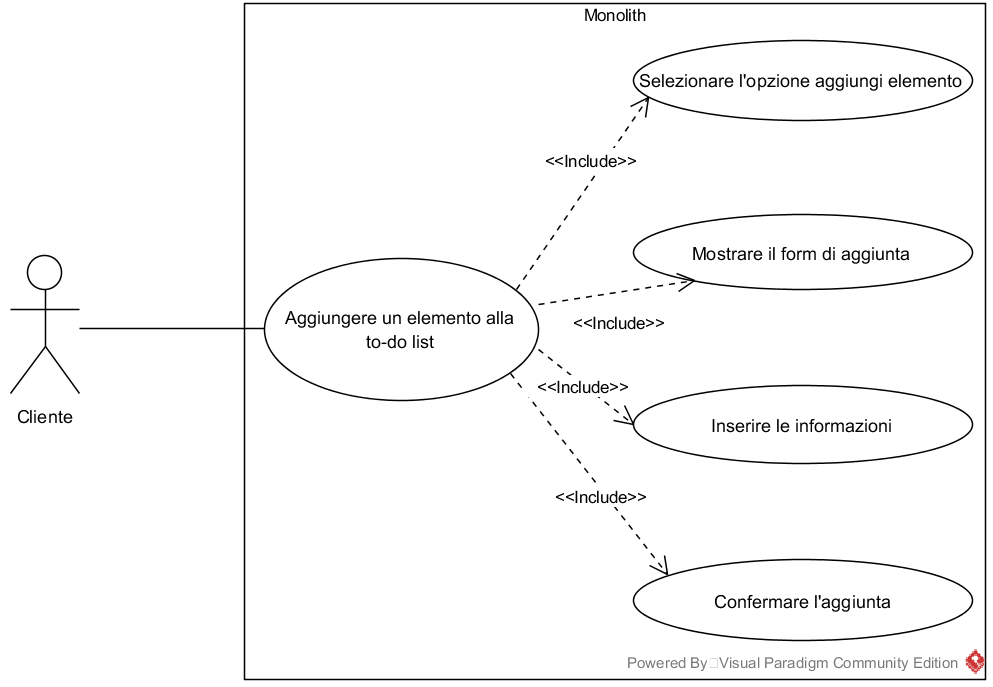
\includegraphics[width=15cm]{../../documenti/AnalisiDeiRequisiti/Diagrammi_img/uc2_2.png}
	\caption{UC2.2 Aggiungere elemento alla to-do list}
\end{figure}

\begin{itemize}
	\item \textbf{Attori:}
	\\Utente di \glossario{Rocket.Chat} in possesso di monolith.
	\item \textbf{Scopo e descrizione:} 
	\\Un utente inserisce un nuovo \glossario{elemento} alla \glossario{to-do list}.
	\item \textbf{Precondizioni:}
	\begin{itemize}
		\item Avere ricevuto una \glossario{bubble} di \glossario{to-do list};
		\item L’\glossario{elemento} non è già stato completato.
	\end{itemize}
	\item \textbf{Flusso principale degli eventi:}
	\begin{itemize}
		\item L'utente seleziona l'opzione aggiungi \glossario{elemento} \hyperref[UC2.2.1]{(UC2.2.1)};
		\item Mostrare il form di aggiunta \hyperref[UC2.2.2]{(UC2.2.2)};
		\item L'utente inserisce le informazioni \hyperref[UC2.2.3]{(UC2.2.3)};
		\item L'utente conferma l'aggiunta \hyperref[UC2.2.4]{(UC2.2.4)}.
	\end{itemize}
	\item \textbf{Post-condizione:}
	\\La \glossario{to-do list} avrà il nuovo \glossario{elemento} aggiunto.
\end{itemize}

\subsubsection{UC2.2.1 Selezionare l'opzione aggiungi elemento} \label{UC2.2.1}

\begin{itemize}
	\item \textbf{Attori:}
	\\Utente di \glossario{Rocket.Chat} in possesso di monolith.
	\item \textbf{Scopo e descrizione:} 
	\\L'utente seleziona l'opzione per inserire un nuovo \glossario{elemento} alla \glossario{to-do list}.
	\item \textbf{Precondizioni:}
	\begin{itemize}
		\item Avere ricevuto una \glossario{bubble} di \glossario{to-do list}.
	\end{itemize}
	\item \textbf{Flusso principale degli eventi:}
	\\L'utilizzatore del metodo seleziona l'opzione apposita.
	\item \textbf{Post-condizione:}
	\\È possibile inserire il testo per il nuovo \glossario{elemento}. 
\end{itemize}

\subsubsection{UC2.2.2 Mostrare il form di aggiunta} \label{UC2.2.2}

\begin{itemize}
	\item \textbf{Attori:}
	\\Utente di \glossario{Rocket.Chat} in possesso di monolith.
	\item \textbf{Scopo e descrizione:} 
	\\Visualizzazione del form di aggiunta delle informazioni relative al nuovo \glossario{elemento} della \glossario{to-do list}.
	\item \textbf{Precondizioni:}
	\begin{itemize}
		\item Avere ricevuto una \glossario{bubble} di \glossario{to-do list};
		\item Avere selezionato l'opzione aggiungi \glossario{elemento} come da \hyperref[UC2.2.1]{UC2.2.1}.
	\end{itemize}
	\item \textbf{Flusso principale degli eventi:}
	\\L'utilizzatore del metodo scrive il testo da inserire nel nuovo \glossario{elemento} e lo aggiunge alla \glossario{to-do list}.
	\item \textbf{Post-condizione:}
	\\Il nuovo \glossario{elemento} è aggiunto alla \glossario{bubble} \glossario{to-do list}.
\end{itemize}

\subsubsection{UC2.2.3  Inserire le informazioni} \label{UC2.2.3}

\begin{itemize}
	\item \textbf{Attori:}
	\\Utente di \glossario{Rocket.Chat} in possesso di monolith.
	\item \textbf{Scopo e descrizione:} 
	\\L'utente inserisce le informazioni necessarie ad aggiungere un \glossario{elemento} alla \glossario{to-do list}.
	\item \textbf{Precondizioni:}
	\begin{itemize}
		\item Avere ricevuto una \glossario{bubble} di \glossario{to-do list};
		\item Aver caricato il form di inserimento secondo lo \hyperref[UC2.2.2]{UC2.2.2};
	\end{itemize}
	\item \textbf{Flusso principale degli eventi:}
	\\L'utilizzatore del metodo completa il form di inserimento di un nuovo \glossario{elemento} in tutte le sue parti.
	\item \textbf{Post-condizione:}
	\\La \glossario{to-do list} ha tutte le informazioni necessarie ad aggiungere il nuovo \glossario{elemento}.
\end{itemize}

\subsubsection{UC2.2.4 Confermare l'aggiunta} \label{UC2.2.4}

\begin{itemize}
	\item \textbf{Attori:}
	\\Utente di \glossario{Rocket.Chat} in possesso di monolith.
	\item \textbf{Scopo e descrizione:} 
	\\Un utente conferma l'inserimento del nuovo \glossario{elemento} alla \glossario{to-do list}.
	\item \textbf{Precondizioni:}
	\begin{itemize}
		\item Avere ricevuto una \glossario{bubble} di \glossario{to-do list};
		\item Aver inserito le informazioni per il nuovo \glossario{elemento} secondo lo \hyperref[UC2.2.3]{UC2.2.3}.
	\end{itemize}
	\item \textbf{Flusso principale degli eventi:}
	\\L'utilizzatore del metodo conferma l'aggiunta alla \glossario{to-do list}.
	\item \textbf{Post-condizione:}
	\\L’\glossario{elemento} è stato aggiunto alla \glossario{to-do list}.
\end{itemize}

\subsubsection{UC2.3 Indicare come completati gli elementi della to-do list} \label{UC2.3}

\begin{figure}[H]
	\centering
	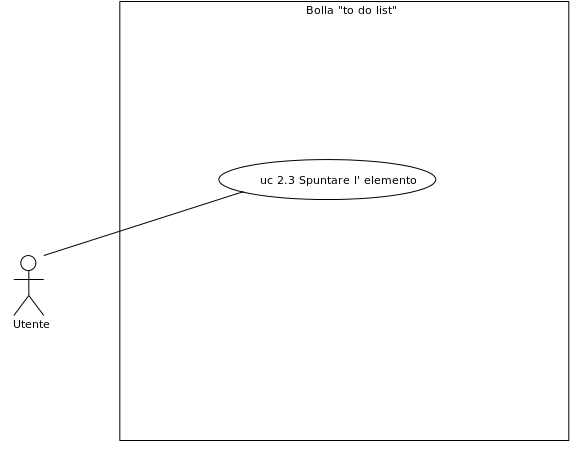
\includegraphics[width=15cm]{../../documenti/AnalisiDeiRequisiti/Diagrammi_img/uc2_3.png}
	\caption{UC2.3 Indicare come completati gli elementi della to-do list}
\end{figure}

\begin{itemize}
	\item \textbf{Attori:}
	\\Utente di \glossario{Rocket.Chat} in possesso di monolith che abbia ricevuto come messaggio una \glossario{bubble} \glossario{to-do list}.
	\item \textbf{Scopo e descrizione:} 
	\\L'utente con questo metodo può indicare come completato uno degli elementi della lista.
	\item \textbf{Precondizioni:}
	\begin{itemize}
		\item Avere ricevuto una \glossario{bubble} di \glossario{to-do list};
		\item L’\glossario{elemento} non è già stato completato.
	\end{itemize}
	\item \textbf{Flusso principale degli eventi:}
	\\L'utilizzatore del metodo seleziona un \glossario{elemento} della \glossario{to-do list} e lo indica come completato. 
	\item \textbf{Post-condizione:}
	\\L’\glossario{elemento} della \glossario{to-do list} viene aggiornato come completato.
\end{itemize}

\subsubsection{UC2.4 Possibilità di mettere un reminder come notifica statica} \label{UC2.4}

\begin{figure}[H]
	\centering
	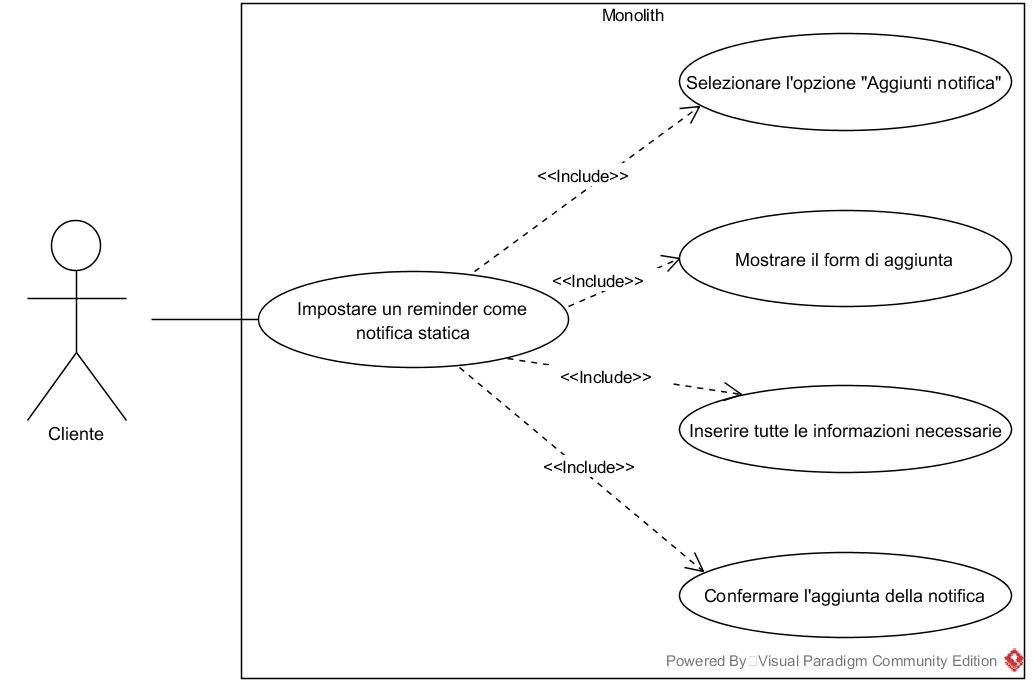
\includegraphics[width=15cm]{../../documenti/AnalisiDeiRequisiti/Diagrammi_img/uc2_4.png}
	\caption{UC2.4 Possibilità di mettere un reminder come notifica statica}
\end{figure}

\begin{itemize}
	\item \textbf{Attori:}
	\\Utente di \glossario{Rocket.Chat} in possesso di monolith che ha creato la \glossario{to-do list}.
	\item \textbf{Scopo e descrizione:} 
	\\Il creatore della lista imposta una notifica statica da visualizzare ai membri del canale ad un orario specificato.
	\item \textbf{Precondizioni:}
	\begin{itemize}
		\item Avere ricevuto una \glossario{bubble} di \glossario{to-do list}.
	\end{itemize}
	\item \textbf{Flusso principale degli eventi:}
	\begin{itemize}
		\item L'utente seleziona l'opzione aggiungi notifica \hyperref[UC2.4.1]{(UC2.4.1)};
		\item Mostrare il form di aggiunta \hyperref[UC2.4.2]{(UC2.4.2)};
		\item L'utente inserisce tutte le informazioni necessarie \hyperref[UC2.4.3]{(UC2.4.3)};
		\item L'utente conferma l'aggiunta della notifica \hyperref[UC2.4.4]{(UC2.4.4)}.
	\end{itemize}
	\item \textbf{Post-condizione:}
	\\I partecipanti al gruppo nel quale è presente la \glossario{bubble} verranno notificati della lista all'ora specificata.
\end{itemize}

\subsubsection{UC2.4.1 Selezionare l'opzione aggiungi notifica} \label{UC2.4.1}

\begin{itemize}
	\item \textbf{Attori:}
	\\Utente di \glossario{Rocket.Chat} in possesso di monolith.
	\item \textbf{Scopo e descrizione:} 
	\\Il creatore della lista seleziona l'opzione “aggiungi notifica”per la \glossario{to-do list} che ha creato.
	\item \textbf{Precondizioni:}
	\begin{itemize}
		\item Avere creato una \glossario{bubble} di \glossario{to-do list}.
	\end{itemize}
	\item \textbf{Flusso principale degli eventi:}
	\\L'utilizzatore del metodo seleziona l'opzione “aggiungi notifica” sulla \glossario{bubble}.
	\item \textbf{Post-condizione:}
	\\L'utente ha selezionato l'opzione di aggiungere una notifica alla \glossario{to-do list} che ha creato.
\end{itemize}

\subsubsection{UC2.4.2 Mostrare il form di aggiunta} \label{UC2.4.2}

\begin{itemize}
	\item \textbf{Attori:}
	\\Utente di \glossario{Rocket.Chat} in possesso di monolith.
	\item \textbf{Scopo e descrizione:} 
	\\Questa funzionalità permette alla \glossario{bubble} di caricare il form necessario ad inserire i dati per aggiungere una notifica alla \glossario{bubble}.
	\item \textbf{Precondizioni:}
	\begin{itemize}
		\item Avere ricevuto una \glossario{bubble} di \glossario{to-do list};
		\item Essere entrati nell'opzione “aggiungi modifica” della propria \glossario{bubble} secondo lo \hyperref[UC2.4.1]{UC2.4.1}.
	\end{itemize}
	\item \textbf{Flusso principale degli eventi:}
	\\La \glossario{bubble} \glossario{to-do list} carica il form di inserimento dati per le notifiche.
	\item \textbf{Post-condizione:}
	\\La \glossario{bubble} ha caricato il form ed è pronta a ricevere in input le informazioni sulla notifica.
\end{itemize}

\subsubsection{UC2.4.3 Inserire tutte le informazioni necessarie} \label{UC2.4.3}

\begin{itemize}
	\item \textbf{Attori:}
	\\Utente di \glossario{Rocket.Chat} in possesso di monolith.
	\item \textbf{Scopo e descrizione:} 
	\\Il creatore della lista completa il form di aggiunta notifica.
	\item \textbf{Precondizioni:}
	\begin{itemize}
		\item Avere ricevuto una \glossario{bubble} di \glossario{to-do list};
		\item La \glossario{bubble} ha caricato il form di inserimento dati secondo lo \hyperref[UC2.4.2]{UC2.4.2}.
	\end{itemize}
	\item \textbf{Flusso principale degli eventi:}
	\\L'utilizzatore del metodo inserirà tutte le informazioni necessarie a completare il form di aggiunta di una notifica.
	\item \textbf{Post-condizione:}
	\\La \glossario{bubble} possiede tutte le informazioni necessarie ad aggiungere una notifica alla \glossario{to-do list}.
\end{itemize}

\subsubsection{UC2.4.4 Confermare l'aggiunta della notifica} \label{UC2.4.4}

\begin{itemize}
	\item \textbf{Attori:}
	\\Utente di \glossario{Rocket.Chat} in possesso di monolith.
	\item \textbf{Scopo e descrizione:} 
	\\Il creatore della lista conferma l'aggiunta della notifica.
	\item \textbf{Precondizioni:}
	\begin{itemize}
		\item Avere ricevuto una \glossario{bubble} di \glossario{to-do list};
		\item Aver completato il form di aggiunta di una notifica secondo lo \hyperref[UC2.4.3]{UC2.4.3}.
	\end{itemize}
	\item \textbf{Flusso principale degli eventi:}
	\\L'utilizzatore del metodo seleziona l'opzione “conferma aggiunta” e la \glossario{bubble} aggiunge la notifica alla lista.
	\item \textbf{Post-condizione:}
	\\La \glossario{bubble} ha aggiunto la notifica alla \glossario{to-do list}.
\end{itemize}

\subsection{Demo}

\subsubsection{Breve descrizione di cosa andiamo a portare alla demo:}
Per la demo del progetto il gruppo orbit presenterà ai proponenti del progetto una \glossario{bubble} interattiva legata alla gestione di un'attività di ristorazione per asporto.
\\Questa \glossario{bubble} apparirà con layout e funzionalità diverse a seconda della tipologia di utente che ne fruirà i servizi.
\\L'utente generico della \glossario{bubble} potrà visualizzare il menu del ristorante e fare un ordine, previo inserimento dei propri dati, inclusivi di indirizzo in cui consegnare il cibo ordinato.
\\L'ordine così effettuato verrà trasmesso alla cucina del locale tramite \glossario{bubble} “todo list”, sotto forma di casella aggiunta automaticamente in fondo alla lista, il \glossario{Cuoco} una volta completato l'ordine avrà facoltà di segnare completata l'ordinazione dalla lista.
\\Contemporaneamente alla notifica alla cucina dell'ordine verrà registrato automaticamente sul database dell'attività il consumo di ingredienti.
\\Qualora la quantità di un ingrediente dovesse scendere al di sotto di una soglia prefissata verrà inviata automaticamente una notifica all'addetto agli acquisti dell'azienda tramite todo list, il quale provvederà a recuperare gli ingredienti mancanti.
\\È prevista anche la figura del \glossario{Direttore} dell'attività il quale avrà facoltà di inserire nuove pietanze nel menù e deciderne il prezzo.

\subsubsection{Attori:}
\begin{itemize}
	\item \glossario{Cliente}: colui che ha facoltà di creare un ordine previa consultazione del menu e registrazione dei propri dati;
	\item \glossario{Cuoco}: addetto alla preparazione della pietanza selezionata in precedenza dall'utente, ha facoltà di eliminare dalla propria to do list le pietanze che ha già preparato;
	\item \glossario{Responsabile Acquisti}: addetto a rifornire il magazzino sulla base degli ingredienti consumati dal \glossario{Cuoco} in base a quanto gli è notificato dalla sua todo list nella \glossario{bubble};
	\item \glossario{Fattorino}: addetto alla consegna delle ordinazioni, ha la facoltà di selezionare le consegne ed eliminarle quando completate;
	\item \glossario{Direttore}: può modificare il menù e il prezzo di ciascuna pietanza riportata in esso.
\end{itemize}

\subsection{Bolla ristorazione per asporto - Cliente}

\subsubsection{UC3.1 Registrazione dei propri dati personali} \label{UC3.1}

\begin{figure}[H]
	\centering
	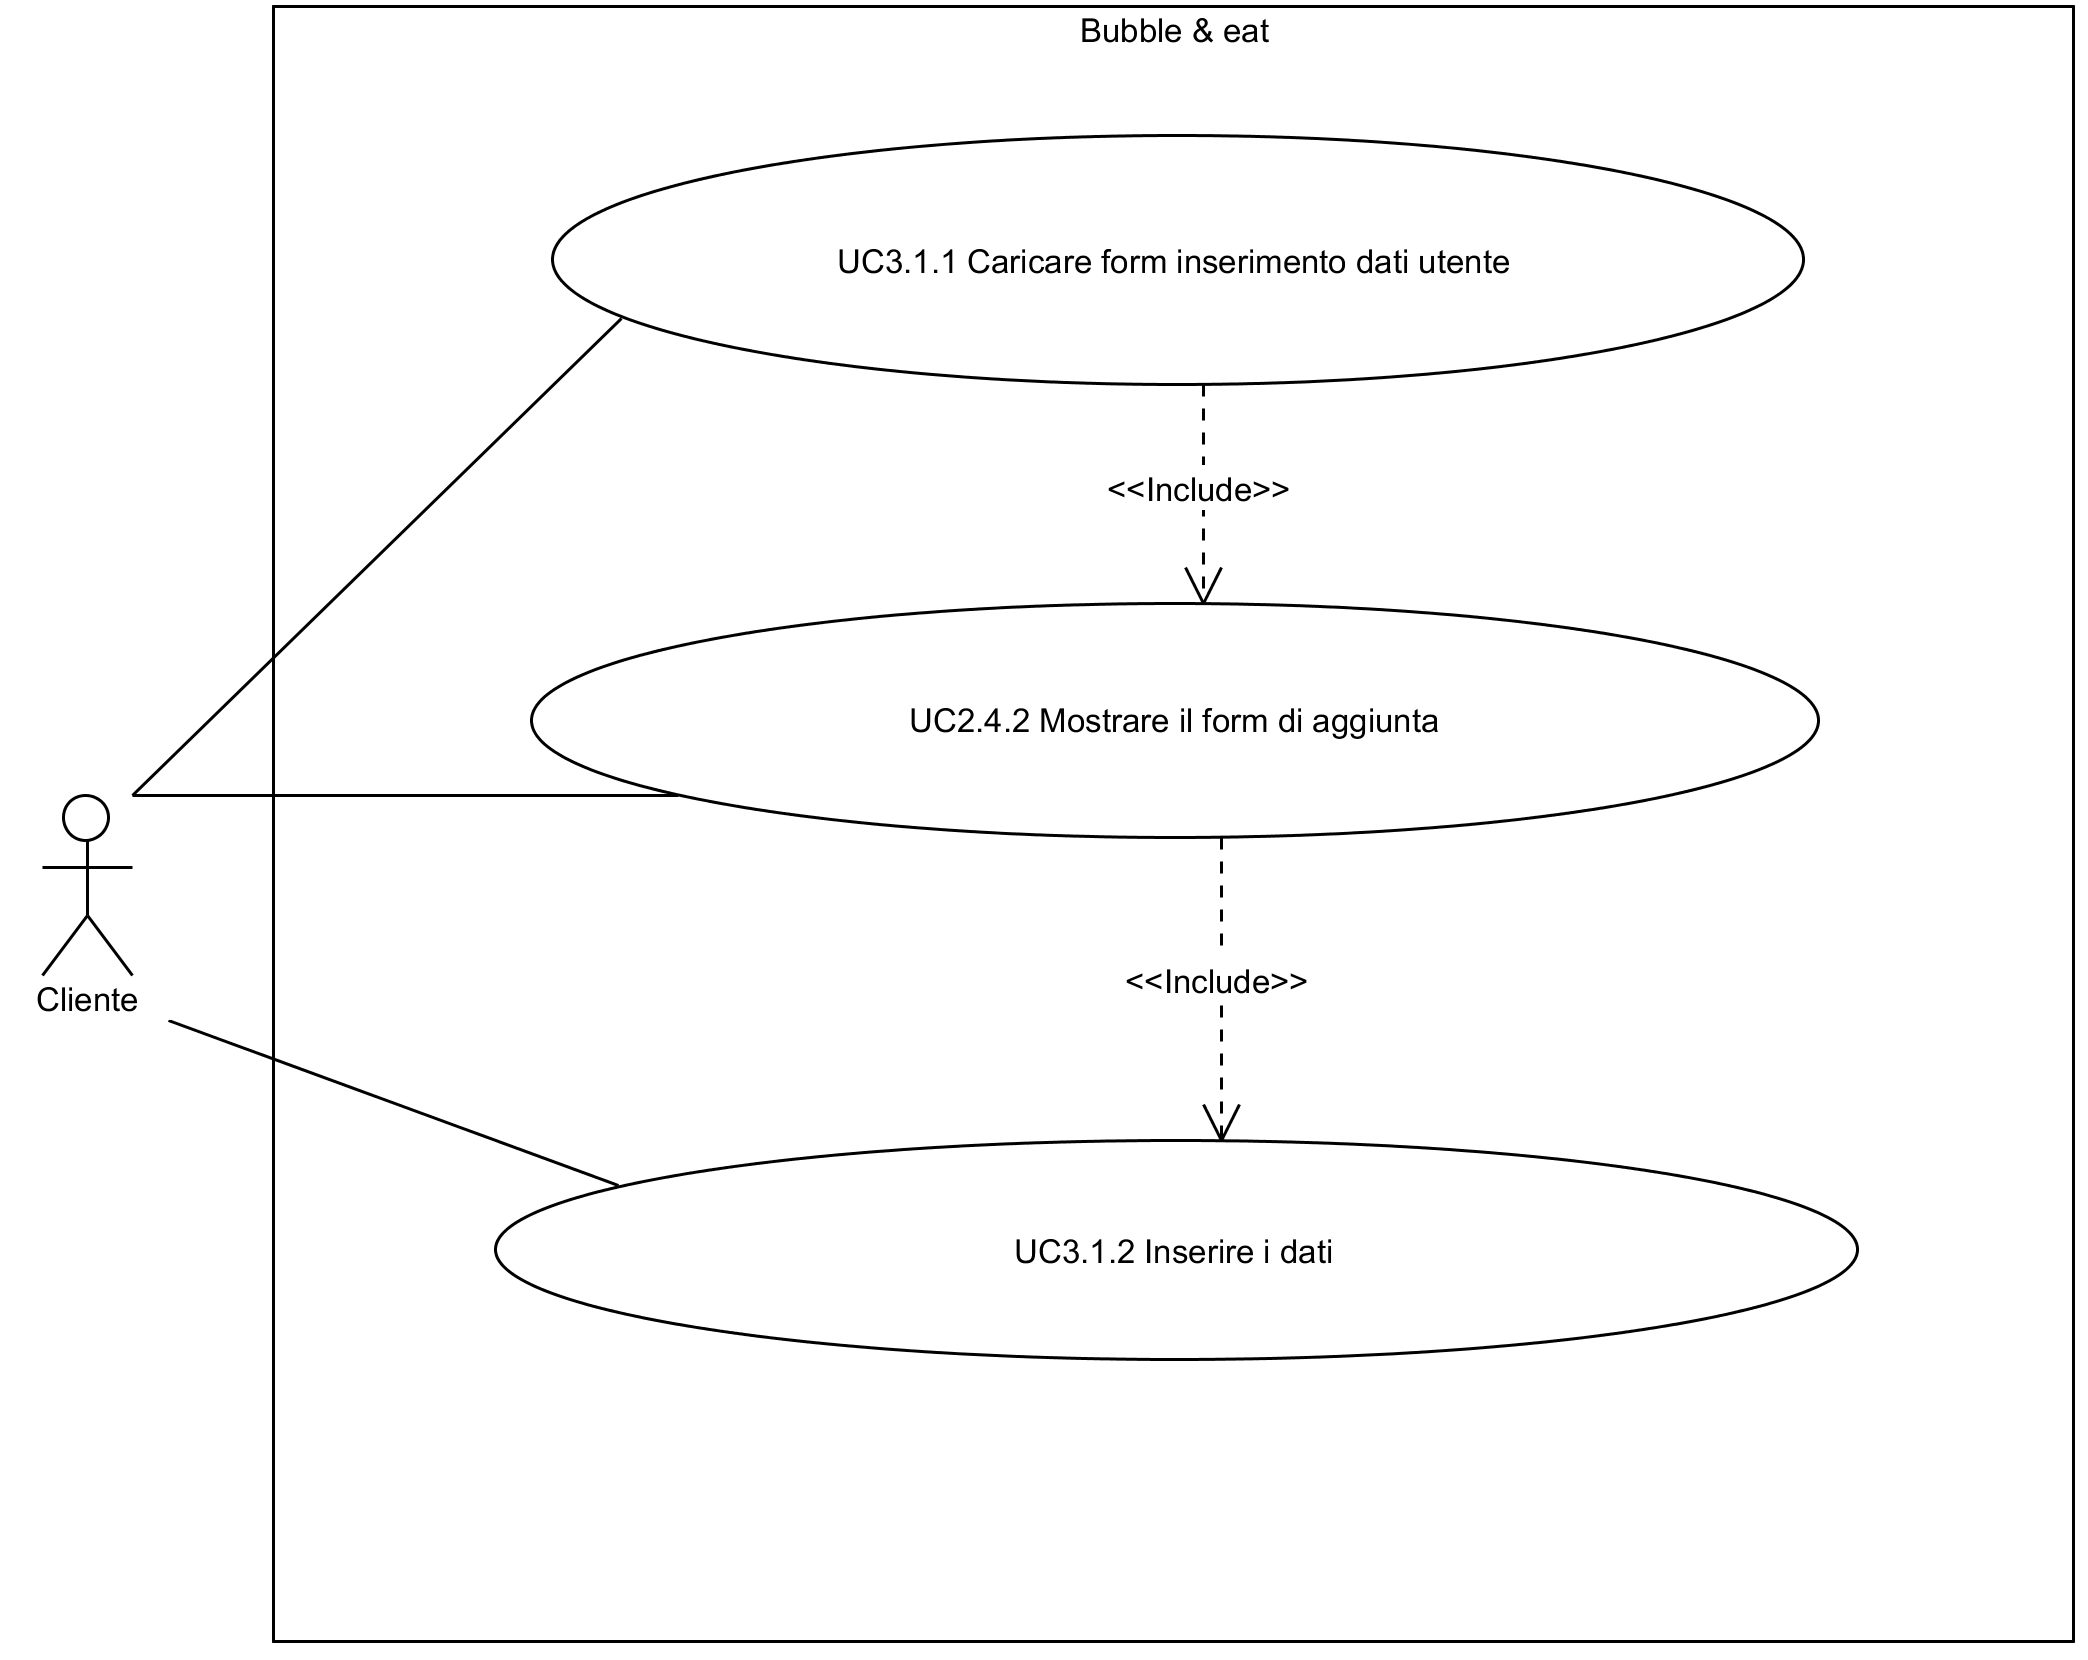
\includegraphics[width=15cm]{../../documenti/AnalisiDeiRequisiti/Diagrammi_img/uc3_1.png}
	\caption{UC3.1 Registrazione dei propri dati personali}
\end{figure}

\begin{itemize}
	\item \textbf{Attori:}
	\\\glossario{Cliente}.
	\item \textbf{Scopo e descrizione:} 
	\\Registrare il proprio indirizzo e il proprio nome e cognome in modo tale da segnalarli all'azienda in maniera tale da avere una destinazione per la spedizione del cibo.
	\item \textbf{Precondizioni:}
	\begin{itemize}
		\item Avere \glossario{Rocket.Chat};
		\item Avere la \glossario{bubble} del ristorante selezionato.
	\end{itemize}
	\item \textbf{Flusso principale degli eventi:}
	\begin{itemize}
		\item Viene caricato il form di inserimento dati dell'utente \hyperref[UC3.1.1]{(UC3.1.1)};
		\item L'utente inserisce i dati \hyperref[UC3.1.2]{(UC3.1.2)};
		\item L'utente conferma l'inserimento \hyperref[UC3.1.3]{(UC3.1.3)}.
	\end{itemize}
	\item \textbf{Post-condizione:}
	\\I dati dell'utente sono stati registrati nella \glossario{bubble memory}.
\end{itemize}

\subsubsection{UC3.1.1 Caricare form inserimento dati utente} \label{UC3.1.1}

\begin{itemize}
	\item \textbf{Attori:}
	\\\glossario{Cliente}.
	\item \textbf{Scopo e descrizione:} 
	\\Dare la possibilità di inserire i propri dati con lo scopo di segnalarli al locale per il corretto funzionamento del servizio.
	\item \textbf{Precondizioni:}
	\begin{itemize}
		\item Avere \glossario{Rocket.Chat};
		\item Avere la \glossario{bubble} del ristorante selezionato.
	\end{itemize}
	\item \textbf{Flusso principale degli eventi:}
	\\Il form per l'inserimento dei dati utente viene caricato.
	\item \textbf{Post-condizione:}
	\\Nella \glossario{bubble} è presente il form per l'inserimento dei dati.
\end{itemize}

\subsubsection{UC3.1.2 Inserire i dati} \label{UC3.1.2}

\begin{itemize}
	\item \textbf{Attori:}
	\\\glossario{Cliente}.
	\item \textbf{Scopo e descrizione:} 
	\\Questo metodo permette all'utente di inserire il proprio indirizzo e il proprio nome e cognome con il fine di segnalarlo all'azienda in maniera tale da avere una destinazione per la spedizione del cibo.
	\item \textbf{Precondizioni:}
	\begin{itemize}
		\item Avere \glossario{Rocket.Chat};
		\item Avere la \glossario{bubble} del ristorante selezionato.
	\end{itemize}
	\item \textbf{Flusso principale degli eventi:}
	\\L'utente seleziona i campi del form di inserimento e digita le informazioni.
	\item \textbf{Post-condizione:}
	\\I dati dell'utente sono stati inseriti.
\end{itemize}

\subsubsection{UC3.1.3 Conferma inserimento} \label{UC3.1.3}

\begin{itemize}
	\item \textbf{Attori:}
	\\\glossario{Cliente}.
	\item \textbf{Scopo e descrizione:} 
	\\Questo metodo permette all'utente di confermare l'inserimento dei dati inseriti nel form di registrazione.
	\item \textbf{Precondizioni:}
	\begin{itemize}
		\item Avere \glossario{Rocket.Chat};
		\item Avere la \glossario{bubble} del ristorante selezionato.
	\end{itemize}
	\item \textbf{Flusso principale degli eventi:}
	\\Con l'apposito comando il \glossario{Cliente} conferma che i dati precedentemente immessi al \glossario{caso d'uso} \hyperref[UC3.1.2]{UC3.1.2} siano corretti.
	\item \textbf{Post-condizione:}
	\\I dati confermati sono presenti nella memoria della \glossario{bubble}.
\end{itemize}

\subsubsection{UC3.2 Guardare il menù} \label{UC3.2}

\begin{figure}[H]
	\centering
	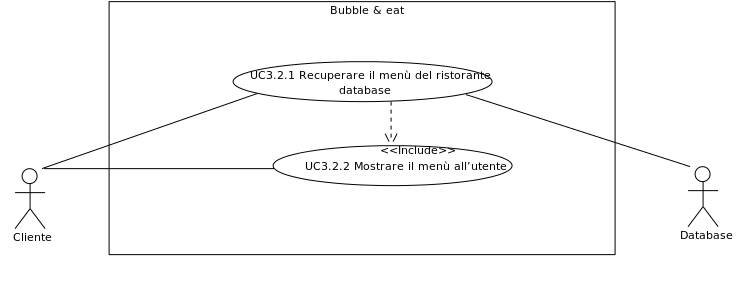
\includegraphics[width=15cm]{../../documenti/AnalisiDeiRequisiti/Diagrammi_img/uc3_2.png}
	\caption{UC3.2 Guardare il menù}
\end{figure}

\begin{itemize}
	\item \textbf{Attori:}
	\\\glossario{Cliente}.
	\item \textbf{Scopo e descrizione:} 
	\\Il \glossario{Cliente} consulta il menu.
	\item \textbf{Precondizioni:}
	\begin{itemize}
		\item Avere \glossario{Rocket.Chat};
		\item Avere la \glossario{bubble} del ristorante selezionato;
		\item Essere loggato nella \glossario{bubble}.
	\end{itemize}
	\item \textbf{Flusso principale degli eventi:}
	\begin{itemize}
		\item Viene recuperato il menù del ristorante dal database \hyperref[UC3.2.1]{(UC3.2.1)};
		\item Il menù caricato viene mostrato all'utente \hyperref[UC3.2.2]{(UC3.2.2)}.
	\end{itemize}
	\item \textbf{Post-condizione:}
	\\Il menu è visualizzato sulla \glossario{bubble}.
\end{itemize}

\subsubsection{UC3.2.1 Recuperare il menù del ristorante dal database} \label{UC3.2.1}

\begin{itemize}
	\item \textbf{Attori:}
	\\\glossario{Cliente}.
	\item \textbf{Scopo e descrizione:} 
	\\Recuperare dal database le voci del menù del ristorante.
	\item \textbf{Precondizioni:}
	\begin{itemize}
		\item Avere \glossario{Rocket.Chat};
		\item Avere la \glossario{bubble} del ristorante selezionato;
		\item Essere loggato nella \glossario{bubble}.
	\end{itemize}
	\item \textbf{Flusso principale degli eventi:}
	\\L'utente invia la richiesta di visualizzazione del menù e la \glossario{bubble} lo carica dal database.
	\item \textbf{Post-condizione:}
	\\Le informazioni sul menù sono state recuperate dalla \glossario{bubble}.
\end{itemize}

\subsubsection{UC3.2.2 Mostrare il menù all'utente} \label{UC3.2.2}

\begin{itemize}
	\item \textbf{Attori:}
	\\\glossario{Cliente}.
	\item \textbf{Scopo e descrizione:} 
	\\Visualizzare il menu nella \glossario{bubble}.
	\item \textbf{Precondizioni:}
	\begin{itemize}
		\item Avere \glossario{Rocket.Chat};
		\item Avere la \glossario{bubble} del ristorante selezionato;
		\item Essere loggato nella \glossario{bubble}.
	\end{itemize}
	\item \textbf{Flusso principale degli eventi:}
	\\Il menù viene mostrato all'utente.
	\item \textbf{Post-condizione:}
	\\Il menù è visualizzato sulla \glossario{bubble}.
\end{itemize}

\subsubsection{UC3.3 Fare le ordinazioni} \label{UC3.3}

\begin{figure}[H]
	\centering
	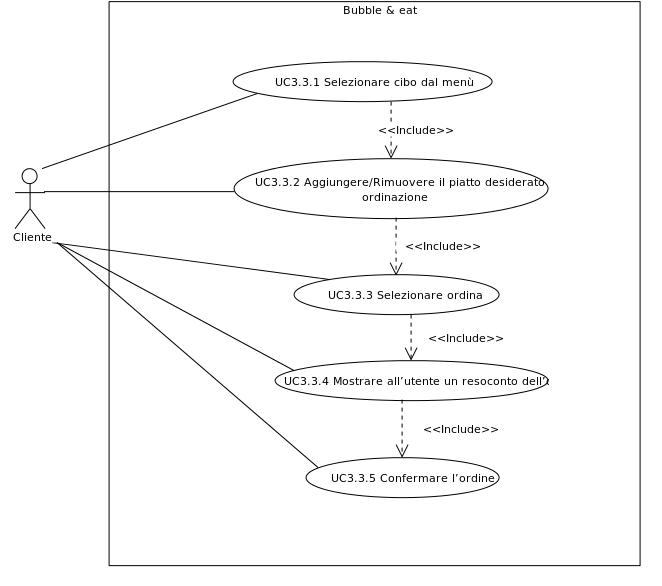
\includegraphics[width=15cm]{../../documenti/AnalisiDeiRequisiti/Diagrammi_img/uc3_3.png}
	\caption{UC3.3 Fare le ordinazioni}
\end{figure}

\begin{itemize}
	\item \textbf{Attori:}
	\\\glossario{Cliente}.
	\item \textbf{Scopo e descrizione:} 
	\\Selezionare il/i piatto/i e le quantità relative ad ogni pietanza.
	\item \textbf{Precondizioni:}
	\begin{itemize}
		\item Avere \glossario{Rocket.Chat};
		\item Avere la \glossario{bubble} del ristorante selezionato;
		\item Essere loggato nella \glossario{bubble}.
	\end{itemize}
	\item \textbf{Flusso principale degli eventi:}
	\begin{itemize}
		\item Visualizzare menù \hyperref[UC3.2]{(UC3.2)};
		\item Selezionare cibi dal menù \hyperref[UC3.3.1]{(UC3.3.1)};
		\item Aggiungere/Rimuovere il cibo selezionato all'ordine \hyperref[UC3.3.2]{(UC3.3.2)};
		\item Selezionare ordina \hyperref[UC3.3.3]{(UC3.3.3)};
		\item Mostrare all'utente un resoconto dell'ordine \hyperref[UC3.3.4]{(UC3.3.4)};
		\item Confermare l'ordine \hyperref[UC3.3.5]{(UC3.3.5)}.
	\end{itemize}
	\item \textbf{Post-condizione:}
	\\L'ordinazione viene aggiornata.
\end{itemize}

\subsubsection{UC3.3.1 Selezionare cibo dal menù} \label{UC3.3.1}

\begin{itemize}
	\item \textbf{Attori:}
	\\\glossario{Cliente}.
	\item \textbf{Scopo e descrizione:} 
	\\Selezionare voce di menù e relativa quantità.
	\item \textbf{Precondizioni:}
	\begin{itemize}
		\item Avere \glossario{Rocket.Chat};
		\item Avere la \glossario{bubble} del ristorante selezionato;
		\item Essere loggato nella \glossario{bubble};
		\item Aver caricato il menù del ristorante \hyperref[UC3.2]{(UC3.2)}.
	\end{itemize}
	\item \textbf{Flusso principale degli eventi:}
	\begin{itemize}
		\item L'utente scorre la lista dei cibi ne seleziona voci e relative quantità.
	\end{itemize}
	\item \textbf{Post-condizione:}
	\\L'utente ha selezionato almeno un piatto dal menù.
\end{itemize}

\subsubsection{UC3.3.2 Aggiungere/Rimuovere il piatto desiderato dall'ordinazione} \label{UC3.3.2}

\begin{itemize}
	\item \textbf{Attori:}
	\\\glossario{Cliente}.
	\item \textbf{Scopo e descrizione:} 
	\\Aggiungere oppure rimuovere alla propria ordinazione una unità del piatto selezionato.
	\item \textbf{Precondizioni:}
	\begin{itemize}
		\item Avere \glossario{Rocket.Chat};
		\item Avere la \glossario{bubble} del ristorante selezionato;
		\item Essere loggato nella \glossario{bubble}.
	\end{itemize}
	\item \textbf{Flusso principale degli eventi:}
	\\L'utente invoca l'apposito comando sulla \glossario{bubble} per poter rimuovere o aggiungere il piatto selezionato al proprio ordine.
	\item \textbf{Post-condizione:}
	\\L'ordinazione viene aggiornata correttamente con il piatto selezionato.
\end{itemize}

\subsubsection{UC3.3.3 Selezionare ordina} \label{UC3.3.3}

\begin{itemize}
	\item \textbf{Attori:}
	\\\glossario{Cliente}.
	\item \textbf{Scopo e descrizione:} 
	\\Il \glossario{Cliente} effettua l'ordine selezionando l'apposita funzione.
	\item \textbf{Precondizioni:}
	\begin{itemize}
		\item Avere \glossario{Rocket.Chat};
		\item Avere la \glossario{bubble} del ristorante selezionato;
		\item Essere loggato nella \glossario{bubble};
		\item Aver selezionato cibi e quantità dal menu \hyperref[UC3.3.1]{(UC3.3.1)} \hyperref[UC3.3.2]{(UC3.3.2)}.
	\end{itemize}
	\item \textbf{Flusso principale degli eventi:}
	\\L'utente invoca l'apposito comando di ordine sulla \glossario{bubble}.
	\item \textbf{Post-condizione:}
	\\L'ordinazione è registrata ed è in attesa di conferma.
\end{itemize}

\subsubsection{UC3.3.4 Mostrare all'utente un resoconto dell'ordine} \label{UC3.3.4}

\begin{itemize}
	\item \textbf{Attori:}
	\\\glossario{Cliente}.
	\item \textbf{Scopo e descrizione:} 
	\\Mostrare all'utente un resoconto dell'ordine che sta per effettuare prima della conferma.
	\item \textbf{Precondizioni:}
	\begin{itemize}
		\item Avere \glossario{Rocket.Chat};
		\item Avere la \glossario{bubble} del ristorante selezionato;
		\item Essere loggato nella \glossario{bubble};
		\item Aver selezionato cibi e quantità dal menu \hyperref[UC3.3.1]{(UC3.3.1)} \hyperref[UC3.3.2]{(UC3.3.2)}.
	\end{itemize}
	\item \textbf{Flusso principale degli eventi:}
	\\L'utente seleziona “Mostra resoconto” e riceve dunque una lista completa di tutto e solo quello che sta per ordinare, insieme al prezzo totale dell'ordine.
	\item \textbf{Post-condizione:}
	\\L'utente visualizza un resoconto dell'ordine prima di effettuarlo.
\end{itemize}

\subsubsection{UC3.3.5 Confermare l'ordine} \label{UC3.3.5}

\begin{itemize}
	\item \textbf{Attori:}
	\\\glossario{Cliente}.
	\item \textbf{Scopo e descrizione:} 
	\\Confermare che quanto mostrato nel \glossario{caso d'uso} \hyperref[UC3.3.4]{UC3.3.4} è corretto e salvare l'ordinazione nella memoria della \glossario{bubble}.
	\item \textbf{Precondizioni:}
	\begin{itemize}
		\item Avere \glossario{Rocket.Chat};
		\item Avere la \glossario{bubble} del ristorante selezionato;
		\item Essere loggato nella \glossario{bubble};
		\item Aver effettuato l'ordinazione \hyperref[UC3.3.4]{(UC3.3.4)}.
	\end{itemize}
	\item \textbf{Flusso principale degli eventi:}
	\\L'utente invoca l'apposito comando sulla \glossario{bubble}.
	\item \textbf{Post-condizione:}
	\\L'ordinazione viene salvata nella memoria della \glossario{bubble}.
\end{itemize}

\subsubsection{UC3.4 Inviare l'ordinazione} \label{UC3.4}

\begin{figure}[H]
	\centering
	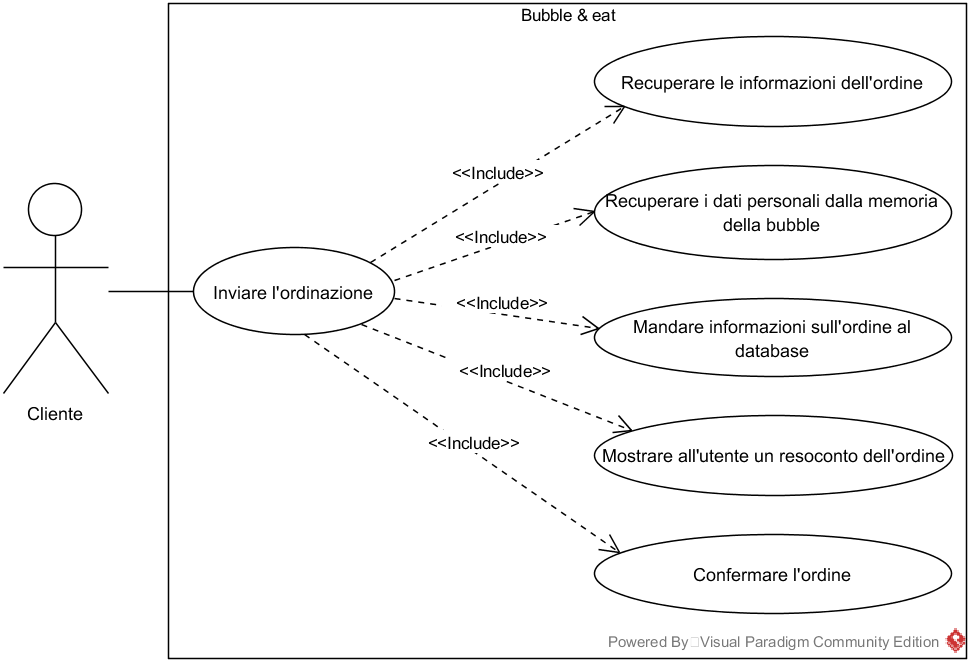
\includegraphics[width=15cm]{../../documenti/AnalisiDeiRequisiti/Diagrammi_img/uc3_4.png}
	\caption{UC3.4 Inviare l'ordinazione}
\end{figure}

\begin{itemize}
	\item \textbf{Attori:}
	\\\glossario{Cliente}.
	\item \textbf{Scopo e descrizione:} 
	\\Selezionare il comando di invio dell'ordinazione.
	\item \textbf{Precondizioni:}
	\begin{itemize}
		\item Avere \glossario{Rocket.Chat};
		\item Avere la \glossario{bubble} del ristorante selezionato;
		\item Essere loggato nella \glossario{bubble};
		\item Avere un ordinazione non vuota.
	\end{itemize}
	\item \textbf{Flusso principale degli eventi:}
	\begin{itemize}
		\item Vengono recuperate dalla memoria della bolla le informazioni sull'ordine \hyperref[UC3.4.1]{(UC3.4.1)};
		\item Vengono recuperate le informazioni sui dati personali del \glossario{Cliente} dalla memoria della bolla \hyperref[UC3.4.2]{(UC3.4.2)};
		\item Vengono inviate le informazioni sull'ordine al database \hyperref[UC3.4.3]{(UC3.4.3)}.
	\end{itemize}
	\item \textbf{Post-condizione:}
	\\L'ordinazione viene inviata.
\end{itemize}

\subsubsection{UC3.4.1 Recuperare le informazioni dell'ordine} \label{UC3.4.1}

\begin{itemize}
	\item \textbf{Attori:}
	\\\glossario{Cliente}.
	\item \textbf{Scopo e descrizione:} 
	\\Prelevare dalla memoria della \glossario{bubble} i dati relativi all'ordinazione confermata nell’\hyperref[UC3.3.5]{UC3.3.5}.
	\item \textbf{Precondizioni:}
	\begin{itemize}
		\item \hyperref[UC3.3.5]{(UC3.3.5)};
		\item Avere \glossario{Rocket.Chat};
		\item Avere la \glossario{bubble} del ristorante selezionato;
		\item Essere loggato nella \glossario{bubble}.
	\end{itemize}
	\item \textbf{Flusso principale degli eventi:}
	\\L'utente invoca con l'apposito comando l’\hyperref[UC3.4]{UC3.4}.
	\item \textbf{Post-condizione:}
	\\I dati desiderati, relativi all'ordinazione effettuata nell’\hyperref[UC3.3]{UC3.3}, sono stati recuperati. 
\end{itemize}

\subsubsection{UC3.4.2 Recuperare informazioni dei dati personali dalla memoria della bubble} \label{UC3.4.2}

\begin{itemize}
	\item \textbf{Attori:}
	\\\glossario{Cliente}.
	\item \textbf{Scopo e descrizione:} 
	\\Ottenere informazioni riguardanti il \glossario{Cliente} dalla memoria della \glossario{bubble}.
	\item \textbf{Precondizioni:}
	\begin{itemize}
		\item Avere \glossario{Rocket.Chat};
		\item Avere la \glossario{bubble} del ristorante selezionato;
		\item Essere loggato nella \glossario{bubble};
		\item Avere un'ordinazione da inviare non vuota.
	\end{itemize}
	\item \textbf{Flusso principale degli eventi:}
	\\Vengono recuperate le informazioni sui dati personali del \glossario{Cliente} dalla memoria della \glossario{bubble}.
	\item \textbf{Post-condizione:}
	\\I dati personali del \glossario{Cliente} sono stati letti dalla memoria della \glossario{bubble}.
\end{itemize}

\subsubsection{UC3.4.3 Mandare informazioni sull'ordine al databese} \label{UC3.4.3}

\begin{itemize}
	\item \textbf{Attori:}
	\\\glossario{Cliente}.
	\item \textbf{Scopo e descrizione:} 
	\\Invio delle informazioni al database.
	\item \textbf{Precondizioni:}
	\begin{itemize}
		\item Avere \glossario{Rocket.Chat};
		\item Avere la \glossario{bubble} del ristorante selezionato;
		\item Essere loggato nella \glossario{bubble};
		\item Avere un ordinazione non vuota.
	\end{itemize}
	\item \textbf{Flusso principale degli eventi:}
	\\Le informazioni sull'ordinazione vengono mandate al database.
	\item \textbf{Post-condizione:}
	\\L'ordinazione è salvata nel database.
\end{itemize}

\subsection{Bolla ristorazione per asporto - Cuoco}

\subsubsection{UC3.5 Leggere la lista dei piatti da preparare} \label{UC3.5}

\begin{figure}[H]
	\centering
	\includegraphics[width=15cm]{../../documenti/AnalisiDeiRequisiti/Diagrammi_img/uc3_5.png}
	\caption{UC3.5 Leggere la lista dei piatti da preparare}
\end{figure}

\begin{itemize}
	\item \textbf{Attori:}
	\\\glossario{Cuoco}.
	\item \textbf{Scopo e descrizione:} 
	\\Lo scopo di questa funzionalità è permettere al \glossario{Cuoco} di consultare la lista dei piatti da preparare ottenuta tramite le ordinazioni effettuate dai clienti.
	\item \textbf{Precondizioni:}
	\begin{itemize}
		\item Avere \glossario{Rocket.Chat};
		\item Avere la \glossario{bubble} del ristorante selezionato;
		\item Avere accesso alla \glossario{bubble} con il ruolo di \glossario{Cuoco}.
	\end{itemize}
	\item \textbf{Flusso principale degli eventi:}
	\begin{itemize}
		\item Il \glossario{Cuoco} seleziona la parte corrispondente della \glossario{bubble};
		\item Viene recuperata dal database la lista dei piatti \hyperref[UC3.5.1]{(UC3.5.1)};
		\item Viene mostrata la lista all'utente \hyperref[UC3.5.2]{(UC3.5.2)}.
	\end{itemize}
	\item \textbf{Post-condizione:}
	\\Il \glossario{Cuoco} è a conoscenza dei piatti ordinati.
\end{itemize}

\subsubsection{UC3.5.1 Recuperare dal database la lista dei piatti} \label{UC3.5.1}

\begin{itemize}
	\item \textbf{Attori:}
	\\\glossario{Cuoco}.
	\item \textbf{Scopo e descrizione:} 
	\\Lo scopo di questa funzionalità è quello di caricare dal database la lista dei piatti da preparare.
	\item \textbf{Precondizioni:}
	\begin{itemize}
		\item Avere \glossario{Rocket.Chat};
		\item Avere la \glossario{bubble} del ristorante selezionato;
		\item Avere accesso alla \glossario{bubble} con il ruolo di \glossario{Cuoco}.
	\end{itemize}
	\item \textbf{Flusso principale degli eventi:}
	\\Il \glossario{Cuoco} richiede di visualizzare la lista dei piatti da preparare, la \glossario{bubble} carica la lista dal database.
	\item \textbf{Post-condizione:}
	\\La \glossario{bubble} ha recuperato la lista dei piatti da preparare dal database.
\end{itemize}

\subsubsection{UC3.5.2 Mostrare la lista} \label{UC3.5.2}

\begin{itemize}
	\item \textbf{Attori:}
	\\\glossario{Cuoco}.
	\item \textbf{Scopo e descrizione:} 
	\\Lo scopo di questa funzionalità è di far visualizzare al \glossario{Cuoco} la lista dei piatti precedentemente caricata dal database sulla \glossario{bubble}.
	\item \textbf{Precondizioni:}
	\begin{itemize}
		\item Avere \glossario{Rocket.Chat};
		\item Avere la \glossario{bubble} del ristorante selezionato;
		\item Avere accesso alla \glossario{bubble} con il ruolo di \glossario{Cuoco};
		\item Aver caricato la lista dei piatti \hyperref[UC3.5.1]{(UC3.5.1)}.
	\end{itemize}
	\item \textbf{Flusso principale degli eventi:}
	\\La \glossario{bubble} mostra la lista dei piatti precedentemente memorizzata al \glossario{Cuoco}.
	\item \textbf{Post-condizione:}
	\\Il \glossario{Cuoco} visualizza la lista dei piatti.
\end{itemize}

\subsubsection{UC3.6 Spunta piatti pronti} \label{UC3.6}

\begin{figure}[H]
	\centering
	\includegraphics[width=15cm]{../../documenti/AnalisiDeiRequisiti/Diagrammi_img/uc3_6.png}
	\caption{UC3.6 Spunta piatti pronti}
\end{figure}

\begin{itemize}
	\item \textbf{Attori:}
	\\\glossario{Cuoco}.
	\item \textbf{Scopo e descrizione:} 
	\\I piatti presenti nella lista possono essere spuntati quando il \glossario{Cuoco} ha finito la loro preparazione.
	\item \textbf{Precondizioni:}
	\begin{itemize}
		\item Avere \glossario{Rocket.Chat};
		\item Avere la \glossario{bubble} del ristorante selezionato;
		\item Avere accesso alla \glossario{bubble} con il ruolo di \glossario{Cuoco};
		\item Avere la lista dei piatti da preparare.
	\end{itemize}
	\item \textbf{Flusso principale degli eventi:}
	\begin{itemize}
		\item Il \glossario{Cuoco} indica che ha terminato la preparazione di un piatto \hyperref[UC3.6.1]{(UC3.6.1)};
		\item Il database viene aggiornato con le nuove informazioni \hyperref[UC3.6.2]{(UC3.6.2)}.
	\end{itemize}
	\item \textbf{Post-condizione:}
	\\Il piatto è stato spuntato.
\end{itemize}

\subsubsection{UC3.6.1 Indicare che la preparazione del piatto è stata completata} \label{UC3.6.1}

\begin{itemize}
	\item \textbf{Attori:}
	\\\glossario{Cuoco}.
	\item \textbf{Scopo e descrizione:} 
	\\Lo scopo di questa funzionalità è di permettere al \glossario{Cuoco} di indicare che ha completato la preparazione di un piatto.
	\item \textbf{Precondizioni:}
	\begin{itemize}
		\item Avere \glossario{Rocket.Chat};
		\item Avere la \glossario{bubble} del ristorante selezionato;
		\item Avere accesso alla \glossario{bubble} con il ruolo di \glossario{Cuoco};
		\item Avere la lista dei piatti da preparare;
		\item Aver precedentemente indicato che si stava preparando un determinato piatto.
	\end{itemize}
	\item \textbf{Flusso principale degli eventi:}
	\\Il \glossario{Cuoco} indica sulla sua lista che ha completato la preparazione del piatto.
	\item \textbf{Post-condizione:}
	\\Il \glossario{Cuoco} ha indicato che ha completato un piatto.
\end{itemize}

\subsubsection{UC3.6.2 Aggiornare il database indicando che il piatto è stato preparato} \label{UC3.6.2}

\begin{itemize}
	\item \textbf{Attori:}
	\\\glossario{Cuoco}.
	\item \textbf{Scopo e descrizione:} 
	\\Lo scopo di questa funzionalità è quello di aggiornare il database in base ai piatti preparati dal \glossario{Cuoco}.
	\item \textbf{Precondizioni:}
	\begin{itemize}
		\item Avere \glossario{Rocket.Chat};
		\item Avere la \glossario{bubble} del ristorante selezionato;
		\item Avere accesso alla \glossario{bubble} con il ruolo di \glossario{Cuoco};
		\item Avere preparato dei piatti dalla lista di piatti da preparare.
	\end{itemize}
	\item \textbf{Flusso principale degli eventi:}
	\\I dati sui piatti preparati dal \glossario{Cuoco} vengono aggiornati nel database.
	\item \textbf{Post-condizione:}
	\\I dati nel database sono aggiornati.
\end{itemize}

\subsection{Bolla ristorazione per asporto - Responsabile Acquisti}

\subsubsection{UC3.7 Leggere la lista degli acquisti da effettuare} \label{UC3.7}

\begin{figure}[H]
	\centering
	\includegraphics[width=15cm]{../../documenti/AnalisiDeiRequisiti/Diagrammi_img/uc3_7.png}
	\caption{UC3.7 Leggere la lista degli acquisti da effettuare}
\end{figure}

\begin{itemize}
	\item \textbf{Attori:}
	\\\glossario{Responsabile Acquisti}.
	\item \textbf{Scopo e descrizione:} 
	\\Lo scopo di questa funzionalità è permettere al \glossario{Responsabile Acquisti} di consulatare la lista degli acquisti da effettuare.
	\item \textbf{Precondizioni:}
	\begin{itemize}
		\item Avere \glossario{Rocket.Chat};
		\item Avere la \glossario{bubble} del ristorante selezionato;
		\item Avere accesso alla \glossario{bubble} con il ruolo di responsabile degli acquisti.
	\end{itemize}
	\item \textbf{Flusso principale degli eventi:}
	\begin{itemize}
		\item Il \glossario{Responsabile Acquisti} seleziona la parte corrispondente della \glossario{bubble};
		\item Viene recuperata dal database la lista degli ingredienti \hyperref[UC3.7.1]{(UC3.7.1)};
		\item La lista viene mostrata all'utente \hyperref[UC3.7.2]{(UC3.7.2)}.
	\end{itemize}
	\item \textbf{Post-condizione:}
	\\Il \glossario{Responsabile Acquisti} è a conoscenza dei prodotti da acquistare.
\end{itemize}

\subsubsection{UC3.7.1 Recuperare dal database la lista degli ingredienti da acquistare con le rispettive quantità} \label{UC3.7.1}

\begin{itemize}
	\item \textbf{Attori:}
	\\\glossario{Responsabile Acquisti}.
	\item \textbf{Scopo e descrizione:} 
	\\Lo scopo di questa funzionalità è di caricare all'interno della \glossario{bubble} la lista degli ingredienti da acquistare con le rispettive quantità.
	\item \textbf{Precondizioni:}
	\begin{itemize}
		\item Avere \glossario{Rocket.Chat};
		\item Avere la \glossario{bubble} del ristorante selezionato;
		\item Avere accesso alla \glossario{bubble} con il ruolo di responsabile degli acquisti.
	\end{itemize}
	\item \textbf{Flusso principale degli eventi:}
	\\Il \glossario{Responsabile Acquisti} richiede di visualizzare la lista e la \glossario{bubble} la carica dal database.
	\item \textbf{Post-condizione:}
	\\La lista degli ingredienti è stata caricata all'interno della \glossario{bubble}.
\end{itemize}

\subsubsection{UC3.7.2 Mostrare la lista al Responsabile Acquisti} \label{UC3.7.2}

\begin{itemize}
	\item \textbf{Attori:}
	\\\glossario{Responsabile Acquisti}.
	\item \textbf{Scopo e descrizione:} 
	\\Lo scopo di questa funzionalità è rendere il responsabile degli acquisti conscio delle quantità e di cosa è incaricato di comprare.
	\item \textbf{Precondizioni:}
	\begin{itemize}
		\item Avere \glossario{Rocket.Chat};
		\item Avere la \glossario{bubble} del ristorante selezionato;
		\item Avere accesso alla \glossario{bubble} con il ruolo di responsabile degli acquisti.
	\end{itemize}
	\item \textbf{Flusso principale degli eventi:}
	\\Il \glossario{Responsabile Acquisti} guarda la \glossario{bubble} interattiva.
	\item \textbf{Post-condizione:}
	\\Il \glossario{Responsabile Acquisti} è a conoscenza dei prodotti da acquistare.
\end{itemize}

\subsubsection{UC3.8 Spunta Acquisti effettuati} \label{UC3.8}

\begin{figure}[H]
	\centering
	\includegraphics[width=15cm]{../../documenti/AnalisiDeiRequisiti/Diagrammi_img/uc3_8.png}
	\caption{UC3.8 Spunta Acquisti effettuati}
\end{figure}

\begin{itemize}
	\item \textbf{Attori:}
	\\\glossario{Responsabile Acquisti}.
	\item \textbf{Scopo e descrizione:} 
	\\Gli acquisti da effettuare presenti nella lista possono essere spuntati quando il \glossario{Responsabile Acquisti} ha acquisito un prodotto nella lista acquisti.
	\item \textbf{Precondizioni:}
	\begin{itemize}
		\item Avere \glossario{Rocket.Chat};
		\item Avere la \glossario{bubble} del ristorante selezionato;
		\item Avere accesso alla \glossario{bubble} con il ruolo di responsabile degli acquisti;
		\item Visualizzare la lista degli acquisti da effettuare \hyperref[UC3.7.2]{(UC3.7.2)}.
	\end{itemize}
	\item \textbf{Flusso principale degli eventi:}
	\\Il \glossario{Responsabile Acquisti} spunta una voce della lista.
	\item \textbf{Post-condizione:}
	\\La voce della lista acquisti è stata spuntata.
\end{itemize}

\subsubsection{UC3.8.1 Spunta degli ingredienti acquistati} \label{UC3.8.1}

\begin{itemize}
	\item \textbf{Attori:}
	\\\glossario{Responsabile Acquisti}.
	\item \textbf{Scopo e descrizione:} 
	\\Questa funzionalità permette al \glossario{Responsabile Acquisti} di segnalare i prodotti acquistati.
	\item \textbf{Precondizioni:}
	\begin{itemize}
		\item Avere \glossario{Rocket.Chat};
		\item Avere la \glossario{bubble} del ristorante selezionato;
		\item Avere accesso alla \glossario{bubble} con il ruolo di responsabile degli acquisti;
		\item Visualizzare la lista degli acquisti da effettuare \hyperref[UC3.7.2]{(UC3.7.2)}.
	\end{itemize}
	\item \textbf{Flusso principale degli eventi:}
	\\I dati vengono inseriti dal \glossario{Responsabile Acquisti}.
	\item \textbf{Post-condizione:}
	\\I dati sono pronti per essere aggiornati nel database.
\end{itemize}

\subsubsection{UC3.8.2 Aggiornare il database con le nuove informazioni} \label{UC3.8.2}

\begin{itemize}
	\item \textbf{Attori:}
	\\\glossario{Responsabile Acquisti}.
	\item \textbf{Scopo e descrizione:} 
	\\Lo scopo di questa funzionalità è quello di registrare all'interno del database i cambiamenti che sono avvenuti nelle quantità degli ingredienti come conseguenza degli acquisti del Responsabile degli acquisti.
	\item \textbf{Precondizioni:}
	\begin{itemize}
		\item Avere \glossario{Rocket.Chat};
		\item Avere la \glossario{bubble} del ristorante selezionato;
		\item Avere accesso alla \glossario{bubble} con il ruolo di responsabile degli acquisti;
		\item Visualizzare la lista degli acquisti da effettuare \hyperref[UC3.7.2]{(UC3.7.2)};
		\item Il Responsabile ha inserito i dati degli ingredienti acquistati.
	\end{itemize}
	\item \textbf{Flusso principale degli eventi:}
	\\Il Responsabile degli acquisti ha inserito i dati degli ingredienti acquistati all'interno della \glossario{bubble}, la quale aggiorna il database.
	\item \textbf{Post-condizione:}
	\\Il database possiede le informazioni aggiornate sulla quantità degli ingredienti.
\end{itemize}

\subsection{Bolla ristorazione per asporto - Fattorino}

\subsubsection{UC3.9 Leggere la lista delle consegne da effettuare} \label{UC3.9}

\begin{figure}[H]
	\centering
	\includegraphics[width=15cm]{../../documenti/AnalisiDeiRequisiti/Diagrammi_img/uc3_9.png}
	\caption{UC3.9 Leggere la lista delle consegne da effettuare}
\end{figure}

\begin{itemize}
	\item \textbf{Attori:}
	\\\glossario{Fattorino}.
	\item \textbf{Scopo e descrizione:} 
	\\Lo scopo di questa funzionalità è permettere al \glossario{Fattorino} di consultare la lista delle consegne da effettuare.
	\item \textbf{Precondizioni:}
	\begin{itemize}
		\item Avere \glossario{Rocket.Chat};
		\item Avere la \glossario{bubble} del ristorante selezionato;
		\item Avere accesso alla \glossario{bubble} con il ruolo \glossario{Fattorino}.
	\end{itemize}
	\item \textbf{Flusso principale degli eventi:}
	\begin{itemize}
		\item Il \glossario{Fattorino} seleziona la parte corrispondente della \glossario{bubble};
		\item Viene recuperata dal database la lista delle consegne \hyperref[UC3.9.1]{(UC3.9.1)};
		\item Viene mostrata la lista all'utente \hyperref[UC3.9.2]{(UC3.9.2)}.
	\end{itemize}
	\item \textbf{Post-condizione:}
	\\Il \glossario{Fattorino} è a conoscenza delle consegne da effettuare.
\end{itemize}

\subsubsection{UC3.9.1 Recuperare dal database la lista delle consegne} \label{UC3.9.1}

\begin{itemize}
	\item \textbf{Attori:}
	\\\glossario{Fattorino}.
	\item \textbf{Scopo e descrizione:} 
	\\Lo scopo di questa funzionalità è avere a disposizione nella memoria della \glossario{bubble} la lista delle consegne da effettuare.
	\item \textbf{Precondizioni:}
	\begin{itemize}
		\item Avere \glossario{Rocket.Chat};
		\item Avere la \glossario{bubble} del ristorante selezionato;
		\item Avere accesso alla \glossario{bubble} con il ruolo \glossario{Fattorino}.
	\end{itemize}
	\item \textbf{Flusso principale degli eventi:}
	\\La \glossario{bubble} salva nella propria memoria la lista delle consegne.
	\item \textbf{Post-condizione:}
	\\Nella memoria della \glossario{bubble} è presente la lista delle consegne da effettuare.
\end{itemize}

\subsubsection{UC3.9.2 Mostrare all'utente la lista} \label{UC3.9.2}

\begin{itemize}
	\item \textbf{Attori:}
	\\\glossario{Fattorino}.
	\item \textbf{Scopo e descrizione:} 
	\\Lo scopo di questa funzionalità è permettere al \glossario{Fattorino} di accedere e leggere la lista delle consegne da effettuare.
	\item \textbf{Precondizioni:}
	\begin{itemize}
		\item Avere \glossario{Rocket.Chat};
		\item Avere la \glossario{bubble} del ristorante selezionato;
		\item Avere accesso alla \glossario{bubble} con il ruolo \glossario{Fattorino}.
	\end{itemize}
	\item \textbf{Flusso principale degli eventi:}
	\\La lista viene visualizzata.
	\item \textbf{Post-condizione:}
	\\La lista è visualizzata, Il \glossario{Fattorino} è a conoscenza delle consegne da effettuare.
\end{itemize}

\subsubsection{UC3.10 Selezionare la consegna da effettuare} \label{UC3.10}

\begin{figure}[H]
	\centering
	\includegraphics[width=15cm]{../../documenti/AnalisiDeiRequisiti/Diagrammi_img/uc3_10.png}
	\caption{UC3.10 Selezionare la consegna da effettuare}
\end{figure}

\begin{itemize}
	\item \textbf{Attori:}
	\\\glossario{Fattorino}.
	\item \textbf{Scopo e descrizione:} 
	\\Lo scopo di questa funzionalità è permettere al \glossario{Fattorino} di selezionare dalla lista delle consegne una da effettuare.
	\item \textbf{Precondizioni:}
	\begin{itemize}
		\item Avere \glossario{Rocket.Chat};
		\item Avere la \glossario{bubble} del ristorante selezionato;
		\item Avere accesso alla \glossario{bubble} con il ruolo \glossario{Fattorino};
		\item Visualizzare la lista delle consegne da effettuare \hyperref[UC3.9.2]{(UC3.9.2)};
		\item Devono esistere consegne da effettuare.
	\end{itemize}
	\item \textbf{Flusso principale degli eventi:}
	\begin{itemize}
		\item Il \glossario{Fattorino} visualizza la lista delle consegne \hyperref[UC3.9]{(UC3.9)};
		\item Il \glossario{Fattorino} seleziona dalla lista quale consegna desidera effettuare \hyperref[UC3.10.1]{(UC3.10.1)};
		\item Il database viene aggiornato per indicare che l'ordine è in consegna \hyperref[UC3.10.2]{(UC3.10.2)}.
	\end{itemize}
	\item \textbf{Post-condizione:}
	\\La lista delle consegne viene aggiornata e viene selezionata la consegna scelta.
\end{itemize}

\subsubsection{UC3.10.1 Selezionare dalla lista la consegna che si vuole effettuare} \label{UC3.10.1}

\begin{itemize}
	\item \textbf{Attori:}
	\\\glossario{Fattorino}.
	\item \textbf{Scopo e descrizione:} 
	\\Lo scopo di questa funzionalità è permettere al \glossario{Fattorino} di selezionare dalla lista delle consegne una da effettuare.
	\item \textbf{Precondizioni:}
	\begin{itemize}
		\item Avere \glossario{Rocket.Chat};
		\item Avere la \glossario{bubble} del ristorante selezionato;
		\item Avere accesso alla \glossario{bubble} con il ruolo \glossario{Fattorino};
		\item Devono esistere consegne da effettuare;
		\item La lista delle consegne da effettuare è visualizzata.
	\end{itemize}
	\item \textbf{Flusso principale degli eventi:}
	\\Il \glossario{Fattorino} seleziona dalla lista quale consegna desidera effettuare.
	\item \textbf{Post-condizione:}
	\\La consegna che il \glossario{Fattorino} vuole effettuare è selezionata.
\end{itemize}

\subsubsection{UC3.10.2 Aggiornare il database per indicare che l'ordine è in consegna} \label{UC3.10.2}

\begin{itemize}
	\item \textbf{Attori:}
	\\\glossario{Fattorino}.
	\item \textbf{Scopo e descrizione:} 
	\\Lo scopo di questa funzionalità è di aggiornare lo stato dell'ordine una volta che il \glossario{Fattorino} l'abbia preso in consegna.
	\item \textbf{Precondizioni:}
	\begin{itemize}
		\item Avere \glossario{Rocket.Chat};
		\item Avere la \glossario{bubble} del ristorante selezionato;
		\item Avere accesso alla \glossario{bubble} con il ruolo \glossario{Fattorino};
		\item Devono esistere consegne da effettuare;
		\item È stata selezionata una consegna da effettuare come indicato nell’\hyperref[UC3.10.1]{(UC3.10.1)}.
	\end{itemize}
	\item \textbf{Flusso principale degli eventi:}
	\\Il \glossario{Fattorino} seleziona dalla lista quale consegna desidera effettuare.
	\item \textbf{Post-condizione:}
	\\L'ordine selezionato nell’\hyperref[UC3.10.1]{(UC3.10.1)} è stato aggiornato nel database cambiandone lo stato in “in consegna”.
\end{itemize}

\subsubsection{UC3.11 Consegna effettuata} \label{UC3.11}

\begin{figure}[H]
	\centering
	\includegraphics[width=15cm]{../../documenti/AnalisiDeiRequisiti/Diagrammi_img/uc3_11.png}
	\caption{UC3.11 Consegna effettuata}
\end{figure}

\begin{itemize}
	\item \textbf{Attori:}
	\\\glossario{Fattorino}.
	\item \textbf{Scopo e descrizione:} 
	\\Lo scopo di questa funzionalità è permettere al \glossario{Fattorino} di confermare l'effettuazione della consegna.
	\item \textbf{Precondizioni:}
	\begin{itemize}
		\item Avere \glossario{Rocket.Chat};
		\item Avere la \glossario{bubble} del ristorante selezionato;
		\item Avere accesso alla \glossario{bubble} con il ruolo \glossario{Fattorino};
		\item Deve essere stata selezionata una consegna dalla lista.
	\end{itemize}
	\item \textbf{Flusso principale degli eventi:}
	\begin{itemize}
		\item Il \glossario{Fattorino} indica che la consegna è stata effettuata \hyperref[UC3.11.1]{(UC3.11.1)};
		\item Il database viene aggiornato \hyperref[UC3.11.2]{(UC3.11.2)}.
	\end{itemize}
	\item \textbf{Post-condizione:}
	\\La lista delle consegne viene aggiornata e viene eliminata la consegna effettuata.
\end{itemize}

\subsubsection{UC3.11.1 Selezionare nella bubble l'opzione per indicare che la consegna è stata effettuata} \label{UC3.11.1}

\begin{itemize}
	\item \textbf{Attori:}
	\\\glossario{Fattorino}.
	\item \textbf{Scopo e descrizione:} 
	\\Lo scopo di questa funzionalità è di notificare l'avvenuta consegna della pietanza all'indirizzo inviato dall'utente.
	\item \textbf{Precondizioni:}
	\begin{itemize}
		\item Avere \glossario{Rocket.Chat};
		\item Avere la \glossario{bubble} del ristorante selezionato;
		\item Avere accesso alla \glossario{bubble} con il ruolo \glossario{Fattorino};
		\item Deve essere stata selezionata una consegna dalla lista;
		\item La consegna deve essere stata effettuata.
	\end{itemize}
	\item \textbf{Flusso principale degli eventi:}
	\\Il \glossario{Fattorino} indica quando la consegna viene portata a termine.
	\item \textbf{Post-condizione:}
	\\Nella \glossario{bubble} del \glossario{Fattorino} è salvato lo stato che la consegna è stata effettuata con successo.
\end{itemize}

\subsubsection{UC3.11.2 Aggiornare il database per mostrare che l'ordine è stato completato} \label{UC3.11.2}

\begin{itemize}
	\item \textbf{Attori:}
	\\\glossario{Fattorino}.
	\item \textbf{Scopo e descrizione:} 
	\\Lo scopo di questa funzionalità è aggiornare il database quando un \glossario{Fattorino} conferma l'effettuazione della consegna.
	\item \textbf{Precondizioni:}
	\begin{itemize}
		\item Avere \glossario{Rocket.Chat};
		\item Avere la \glossario{bubble} del ristorante selezionato;
		\item Avere accesso alla \glossario{bubble} con il ruolo \glossario{Fattorino};
		\item Deve essere stata selezionata una consegna dalla lista per essere segnata come completata.
	\end{itemize}
	\item \textbf{Flusso principale degli eventi:}
	\\Vengono aggiornati i dati nel database quando una consegna viene confermata.
	\item \textbf{Post-condizione:}
	\\I dati nel database sono aggiornati.
\end{itemize}

\subsection{Bolla ristorazione per asporto - Direttore}

\subsubsection{UC3.12 Cancellare ordini al Cuoco} \label{UC3.12}

\begin{figure}[H]
	\centering
	\includegraphics[width=15cm]{../../documenti/AnalisiDeiRequisiti/Diagrammi_img/uc3_12.png}
	\caption{UC3.12 Cancellare ordini al Cuoco}
\end{figure}

\begin{itemize}
	\item \textbf{Attori:}
	\\\glossario{Direttore}.
	\item \textbf{Scopo e descrizione:} 
	\\Lo scopo di questa funzione è permettere al \glossario{Direttore} di cancellare ordini dalla \glossario{to-do list} del \glossario{Cuoco}.
	\item \textbf{Precondizioni:}
	\begin{itemize}
		\item Avere \glossario{Rocket.Chat};
		\item Avere la \glossario{bubble} del ristorante selezionato;
		\item Avere accesso alla \glossario{bubble} con il ruolo di \glossario{Direttore}.
	\end{itemize}
	\item \textbf{Flusso principale degli eventi:}
	\begin{itemize}
		\item Recuperare dal database la lista degli ordini \hyperref[UC3.12.1]{(UC3.12.1)};
		\item Visualizzare lista ordini \hyperref[UC3.12.2]{(UC3.12.2)};
		\item L'utente \glossario{Direttore} seleziona dalla lista gli ordini che desidera rimuovere \hyperref[UC3.12.3]{(UC3.12.3)};
		\item L'utente \glossario{Direttore} seleziona l'opzione per rimuovere gli ordini selezionati \hyperref[UC3.12.4]{(UC3.12.4)};
		\item L'utente \glossario{Direttore} seleziona l'opzione per confermare \hyperref[UC3.12.5]{(UC3.12.5)};
		\item Aggiornare il database \hyperref[UC3.12.6]{(UC3.12.6)}.
	\end{itemize}
	\item \textbf{Post-condizione:}
	\\L'ordine è stato cancellato dalla \glossario{to-do list} del \glossario{Cuoco}.
\end{itemize}

\subsubsection{UC3.12.1 Recuperare dal database la lista degli ordini(Direttore)} \label{UC3.12.1}

\begin{itemize}
	\item \textbf{Attori:}
	\\\glossario{Direttore}.
	\item \textbf{Scopo e descrizione:} 
	\\Lo scopo di questa funzione è permettere alla \glossario{bubble} del \glossario{Direttore} di avere nella propria memoria la lista delle ordinazioni effettuate.
	\item \textbf{Precondizioni:}
	\begin{itemize}
		\item Avere \glossario{Rocket.Chat};
		\item Avere la \glossario{bubble} del ristorante selezionato;
		\item Avere accesso alla \glossario{bubble} con il ruolo di \glossario{Direttore}.
	\end{itemize}
	\item \textbf{Flusso principale degli eventi:}
	\\Il \glossario{Direttore} consulta la \glossario{bubble} in modalità di cancellazione dell'ordinazione del \glossario{Cuoco}.
	\item \textbf{Post-condizione:}
	\\L'ordine è stato cancellato dalla \glossario{to-do list} del \glossario{Cuoco}.
\end{itemize}

\subsubsection{UC3.12.2 Visualizzare lista ordini(Direttore)} \label{UC3.12.2}

\begin{itemize}
	\item \textbf{Attori:}
	\\\glossario{Direttore}.
	\item \textbf{Scopo e descrizione:} 
	\\Lo scopo di questa funzione è permettere al \glossario{Direttore} di cancellare ordini dalla \glossario{to-do list} del \glossario{Cuoco}.
	\item \textbf{Precondizioni:}
	\begin{itemize}
		\item Avere \glossario{Rocket.Chat};
		\item Avere la \glossario{bubble} del ristorante selezionato;
		\item Avere accesso alla \glossario{bubble} con il ruolo di \glossario{Direttore}.
	\end{itemize}
	\item \textbf{Flusso principale degli eventi:}
	\\Il \glossario{Direttore} visualizza la lista degli ordini per poterne rimuovere.
	\item \textbf{Post-condizione:}
	\\La lista degli ordini è visualizzata.
\end{itemize}

\subsubsection{UC3.12.3 Selezionare dalla lista gli ordini che si desidera rimuovere} \label{UC3.12.3}

\begin{itemize}
	\item \textbf{Attori:}
	\\\glossario{Direttore}.
	\item \textbf{Scopo e descrizione:} 
	\\Lo scopo di questa funzione è permettere al \glossario{Direttore} di selezionare ordini da cancellare dalla \glossario{to-do list} del \glossario{Cuoco}.
	\item \textbf{Precondizioni:}
	\begin{itemize}
		\item Avere \glossario{Rocket.Chat};
		\item Avere la \glossario{bubble} del ristorante selezionato;
		\item Avere accesso alla \glossario{bubble} con il ruolo di \glossario{Direttore};
		\item La lista degli ordini da eliminare è visualizzata.
	\end{itemize}
	\item \textbf{Flusso principale degli eventi:}
	\\Il \glossario{Direttore} sceglie l'ordine da eliminare dalla \glossario{to-do list} del \glossario{Cuoco}.
	\item \textbf{Post-condizione:}
	\\Sono stati selezionati degli ordini dalla lista.
\end{itemize}

\subsubsection{UC3.12.4 Selezionare l'opzione per rimuovere gli ordini selezionati} \label{UC3.12.4}

\begin{itemize}
	\item \textbf{Attori:}
	\\\glossario{Direttore}.
	\item \textbf{Scopo e descrizione:} 
	\\Lo scopo di questa funzione è permettere al \glossario{Direttore} di eliminare gli ordini selezionati per l'eliminazione.
	\item \textbf{Precondizioni:}
	\begin{itemize}
		\item Avere \glossario{Rocket.Chat};
		\item Avere la \glossario{bubble} del ristorante selezionato;
		\item Avere accesso alla \glossario{bubble} con il ruolo di \glossario{Direttore};
		\item Sono stati selezionati ordini da eliminare \hyperref[UC3.12.3]{(UC3.12.3)}.
	\end{itemize}
	\item \textbf{Flusso principale degli eventi:}
	\\Il \glossario{Direttore} sceglie l'ordine da eliminare dalla \glossario{to-do list} del \glossario{Cuoco}.
	\item \textbf{Post-condizione:}
	\\L'ordine da cancellare è selezionato.
\end{itemize}

\subsubsection{UC3.12.5 Selezionare l'opzione per confermare la rimozione degli ordini selezionati} \label{UC3.12.5}

\begin{itemize}
	\item \textbf{Attori:}
	\\\glossario{Direttore}.
	\item \textbf{Scopo e descrizione:} 
	\\Lo scopo di questa funzione è permettere al \glossario{Direttore} di confermare la selezione degli ordini da eliminare.
	\item \textbf{Precondizioni:}
	\begin{itemize}
		\item Avere \glossario{Rocket.Chat};
		\item Avere la \glossario{bubble} del ristorante selezionato;
		\item Avere accesso alla \glossario{bubble} con il ruolo di \glossario{Direttore};
		\item La lista degli ordini da eliminare è visualizzata;
		\item E stata selezionata l'eliminazione di ordini selezionati \hyperref[UC3.12.4]{(UC3.12.4)}.
	\end{itemize}
	\item \textbf{Flusso principale degli eventi:}
	\\Il \glossario{Direttore} sceglie l'ordine da eliminare dalla \glossario{to-do list} del \glossario{Cuoco}.
	\item \textbf{Post-condizione:}
	\\Il \glossario{Direttore} ha confermato quale ordine cancellare.
\end{itemize}

\subsubsection{UC3.12.6 Aggiornare il database} \label{UC3.12.6}

\begin{itemize}
	\item \textbf{Attori:}
	\\\glossario{Direttore}.
	\item \textbf{Scopo e descrizione:} 
	\\Lo scopo di questa funzione aggiornare il database in base agli ordini cancellati dal \glossario{Direttore}.
	\item \textbf{Precondizioni:}
	\begin{itemize}
		\item Avere \glossario{Rocket.Chat};
		\item Avere la \glossario{bubble} del ristorante selezionato;
		\item Avere accesso alla \glossario{bubble} con il ruolo di \glossario{Direttore};
		\item Avere confermato quali ordini eliminare \hyperref[UC3.12.5]{(UC3.12.5)}.
	\end{itemize}
	\item \textbf{Flusso principale degli eventi:}
	\\Vengono aggiornati nel database i dati relativi agli ordini da eliminare.
	\item \textbf{Post-condizione:}
	\\L'ordine è stato cancellato dalla \glossario{to-do list} del \glossario{Cuoco}.
\end{itemize}

\subsubsection{UC3.13 Cambiare il menù} \label{UC3.13}

\begin{figure}[H]
	\centering
	\includegraphics[width=15cm]{../../documenti/AnalisiDeiRequisiti/Diagrammi_img/uc3_13.png}
	\caption{UC3.13 Cambiare il menù}
\end{figure}

\begin{itemize}
	\item \textbf{Attori:}
	\\\glossario{Direttore}.
	\item \textbf{Scopo e descrizione:} 
	\\Permettere all'utente \glossario{Direttore} di modificare il menu del ristorante.
	\item \textbf{Precondizioni:}
	\begin{itemize}
		\item Avere \glossario{Rocket.Chat};
		\item Avere la \glossario{bubble} del ristorante selezionato;
		\item Avere accesso alla \glossario{bubble} con il ruolo di \glossario{Direttore}.
	\end{itemize}
	\item \textbf{Flusso principale degli eventi:}
	\begin{itemize}
		\item Il \glossario{Direttore} visualizza il menù \hyperref[UC3.13.1]{(UC3.13.1)};
		\item Il \glossario{Direttore} elimina degli elementi dal menù \hyperref[UC3.13.2]{(UC3.13.2)};
		\item Il \glossario{Direttore} modifica degli elementi del menù \hyperref[UC3.13.3]{(UC3.13.3)};
		\item Il \glossario{Direttore} aggiunge elementi al menù \hyperref[UC3.13.4]{(UC3.13.4)}.
	\end{itemize}
	\item \textbf{Post-condizione:}
	\\Il menù è modificato.
\end{itemize}

\subsubsection{UC3.13.1 Visualizzare il menù del ristorante(Direttore)} \label{UC3.13.1}

\begin{figure}[H]
	\centering
	\includegraphics[width=15cm]{../../documenti/AnalisiDeiRequisiti/Diagrammi_img/uc3_13_1.png}
	\caption{UC3.13.1 Visualizzare il menù del ristorante(Direttore)}
\end{figure}

\begin{itemize}
	\item \textbf{Attori:}
	\\\glossario{Direttore}.
	\item \textbf{Scopo e descrizione:} 
	\\Lo scopo di questa funzionalità è di mostrare al \glossario{Direttore} il menù.
	\item \textbf{Precondizioni:}
	\begin{itemize}
		\item Avere \glossario{Rocket.Chat};
		\item Avere la \glossario{bubble} del ristorante selezionato;
		\item Avere accesso alla \glossario{bubble} con il ruolo di \glossario{Direttore}.
	\end{itemize}
	\item \textbf{Flusso principale degli eventi:}
	\begin{itemize}
		\item Viene recuperato dal database il menù del ristorante \hyperref[UC3.13.1.1]{(UC3.13.1.1)};
		\item Viene mostrato all'utente il menù \hyperref[UC3.13.1.2]{(UC3.13.1.2)}.
	\end{itemize}
	\item \textbf{Post-condizione:}
	\\Nella \glossario{bubble memory} è presente il menù.
\end{itemize}

\subsubsection{UC3.13.1.1 Recuperare dal database il menù del ristorante (Direttore)} \label{UC3.13.1.1}

\begin{itemize}
	\item \textbf{Attori:}
	\\\glossario{Direttore}.
	\item \textbf{Scopo e descrizione:} 
	\\Recuperare il menu del ristorante dal database.
	\item \textbf{Precondizioni:}
	\begin{itemize}
		\item Avere \glossario{Rocket.Chat};
		\item Avere la bubble del ristorante selezionato;
		\item Avere accesso alla bubble con il ruolo di \glossario{Direttore}.
	\end{itemize}
	\item \textbf{Flusso principale degli eventi:}
	\\Il \glossario{Direttore} accede alla sezione di modifica del menù della sua bubble.
	\item \textbf{Post-condizione:}
	\\Nella \glossario{bubble memory} è presente il menu.
\end{itemize}

\subsubsection{UC3.13.1.2 Visualizzare il menu (Direttore)} \label{UC3.13.1.2}

\begin{itemize}
	\item \textbf{Attori:}
	\\\glossario{Direttore}.
	\item \textbf{Scopo e descrizione:} 
	\\Il \glossario{Direttore} deve poter visualizzare il menu per poterlo modificare.
	\item \textbf{Precondizioni:}
	\begin{itemize}
		\item Avere \glossario{Rocket.Chat};
		\item Avere la bubble del ristorante selezionato;
		\item Avere accesso alla bubble con il ruolo di \glossario{Direttore};
		\item Aver recuperato le informazioni dal database \hyperref[UC3.13.1.1]{(UC3.13.1.1)}.
	\end{itemize}
	\item \textbf{Flusso principale degli eventi:}
	\\Il \glossario{Direttore} si trova nel menù.
	\item \textbf{Post-condizione:}
	\\Il menu è visualizzato.
\end{itemize}

\subsubsection{UC3.13.2 Eliminare elementi dal menù} \label{UC3.13.2}

\begin{figure}[H]
	\centering
	\includegraphics[width=15cm]{../../documenti/AnalisiDeiRequisiti/Diagrammi_img/uc3_13_2.png}
	\caption{UC3.13.2 Eliminare elementi dal menù}
\end{figure}

\begin{itemize}
	\item \textbf{Attori:}
	\\\glossario{Direttore}.
	\item \textbf{Scopo e descrizione:} 
	\\Lo scopo di questa funzionalità è di eliminare elementi dal menù.
	\item \textbf{Precondizioni:}
	\begin{itemize}
		\item Avere \glossario{Rocket.Chat};
		\item Avere la bubble del ristorante selezionato;
		\item Avere accesso alla bubble con il ruolo di \glossario{Direttore};
		\item Aver visualizzato il menù del ristorante \hyperref[UC3.13.1]{(UC3.13.1)}.
	\end{itemize}
	\item \textbf{Flusso principale degli eventi:}
	\begin{itemize}
		\item Il \glossario{Direttore} seleziona dal menù i cibi che desidera togliere \hyperref[UC3.13.2.1]{(UC3.13.2.1)};
		\item Il \glossario{Direttore} conferma l'operazione \hyperref[UC3.13.2.2]{(UC3.13.2.2)};
		\item Il database viene aggiornato \hyperref[UC3.13.2.3]{(UC3.13.2.3)}.
	\end{itemize}
	\item \textbf{Post-condizione:}
	\\Gli elementi desiderati sono stati eliminati dal menù.
\end{itemize}

\subsubsection{UC3.13.2.1 Selezionare dal menù i cibi che si desidera rimuovere} \label{UC3.13.2.1}

\begin{itemize}
	\item \textbf{Attori:}
	\\\glossario{Direttore}.
	\item \textbf{Scopo e descrizione:} 
	\\Avere una selezione di voci da rimuovere dal menu.
	\item \textbf{Precondizioni:}
	\begin{itemize}
		\item Avere \glossario{Rocket.Chat};
		\item Avere la bubble del ristorante selezionato;
		\item Avere accesso alla bubble con il ruolo di \glossario{Direttore};
		\item Aver visualizzato il menù del ristorante \hyperref[UC3.13.1]{(UC3.13.1)}.
	\end{itemize}
	\item \textbf{Flusso principale degli eventi:}
	\\Il \glossario{Direttore} seleziona dalla lista visualizzata nell'\hyperref[UC3.13.1]{(UC3.13.1)} gli elementi del menu che desidera rimuovere da esso.
	\item \textbf{Post-condizione:}
	\\Gli elementi sono stati selezionati.
\end{itemize}

\subsubsection{UC3.13.2.2 Selezionare l'opzione per rimuovere gli elementi selezionati} \label{UC3.13.2.2}

\begin{itemize}
	\item \textbf{Attori:}
	\\\glossario{Direttore}.
	\item \textbf{Scopo e descrizione:} 
	\\Rimuovere gli elementi selezionati con l'apposita opzione.
	\item \textbf{Precondizioni:}
	\begin{itemize}
		\item Avere \glossario{Rocket.Chat};
		\item Avere la bubble del ristorante selezionato;
		\item Avere accesso alla bubble con il ruolo di \glossario{Direttore};
		\item Aver visualizzato il menù del ristorante \hyperref[UC3.13.1]{(UC3.13.1)}.
	\end{itemize}
	\item \textbf{Flusso principale degli eventi:}
	\\Il \glossario{Direttore} si trova nel menù, ha selezionato gli elementi da eliminare, e ne conferma l'eliminazione.
	\item \textbf{Post-condizione:}
	\\Gli elementi sono eliminati dal menu.
\end{itemize}

\subsubsection{UC3.13.2.3 Aggiornare il database} \label{UC3.13.2.3}

\begin{itemize}
	\item \textbf{Attori:}
	\\\glossario{Direttore}.
	\item \textbf{Scopo e descrizione:} 
	\\Notificare al sistema l'aggiornamento del menu effettuato allo \hyperref[UC3.13.2.2]{(UC3.13.2.2)}.
	\item \textbf{Precondizioni:}
	\begin{itemize}
		\item Avere \glossario{Rocket.Chat};
		\item Avere la bubble del ristorante selezionato;
		\item Avere accesso alla bubble con il ruolo di \glossario{Direttore};
		\item Aver selezionato l'opzione per rimuovere gli elementi selezionati dal menu \hyperref[UC3.13.2.2]{(UC3.13.2.2)}.
	\end{itemize}
	\item \textbf{Flusso principale degli eventi:}
	\\Il \glossario{Direttore} ha confermato l'eliminazione dal menu degli elementi selezionati in precedenza.
	\item \textbf{Post-condizione:}
	\\La modifica del menù è stata propagata al database.
\end{itemize}

\subsubsection{UC3.13.3 Modificare elementi del menù} \label{UC3.13.3}

\begin{figure}[H]
	\centering
	\includegraphics[width=15cm]{../../documenti/AnalisiDeiRequisiti/Diagrammi_img/uc3_13_3.png}
	\caption{UC3.13.3 Modificare elementi del menù}
\end{figure}

\begin{itemize}
	\item \textbf{Attori:}
	\\\glossario{Direttore}.
	\item \textbf{Scopo e descrizione:} 
	\\Lo scopo di questa funzionalità è di permettere al \glossario{Direttore} di modificare elementi del menù.
	\item \textbf{Precondizioni:}
	\begin{itemize}
		\item Avere \glossario{Rocket.Chat};
		\item Avere la bubble del ristorante selezionato;
		\item Avere accesso alla bubble con il ruolo di \glossario{Direttore};
		\item Aver visualizzato il menù del ristorante \hyperref[UC3.13.1]{(UC3.13.1)}.
	\end{itemize}
	\item \textbf{Flusso principale degli eventi:}
	\begin{itemize}
		\item Il \glossario{Direttore} seleziona dal menù l’\glossario{elemento} che desidera modificare \hyperref[UC3.13.3.1]{(UC3.13.3.1)};
		\item Viene confermata la selezione \hyperref[UC3.13.3.2]{(UC3.13.3.2)};
		\item Il \glossario{Direttore} inserisce le nuove informazioni \hyperref[UC3.13.3.3]{(UC3.13.3.3)};
		\item Vengono confermati i cambiamenti \hyperref[UC3.13.3.4]{(UC3.13.3.4)};
		\item Il database viene aggiornato \hyperref[UC3.13.3.5]{(UC3.13.3.5)}.
	\end{itemize}
	\item \textbf{Post-condizione:}
	\\Sono state applicate le modifiche desiderate agli elementi del menù.
\end{itemize}

\subsubsection{UC3.13.3.1  Selezionare dal menù il cibo che si desidera modificare} \label{UC3.13.3.1}

\begin{itemize}
	\item \textbf{Attori:}
	\\\glossario{Direttore}.
	\item \textbf{Scopo e descrizione:} 
	\\Permettere all'utente \glossario{Direttore} di modificare voci del menu.
	\item \textbf{Precondizioni:}
	\begin{itemize}
		\item Avere \glossario{Rocket.Chat};
		\item Avere la bubble del ristorante selezionato;
		\item Avere accesso alla bubble con il ruolo di \glossario{Direttore}.
	\end{itemize}
	\item \textbf{Flusso principale degli eventi:}
	\\Il \glossario{Direttore} si trova nel menù, può selezionare la voce del menu da modificare.
	\item \textbf{Post-condizione:}
	\\Le voci sono selezionate.
\end{itemize}

\subsubsection{UC3.13.3.2 Selezionare l'opzione per modificare il la voce del menu selezionata} \label{UC3.13.3.2}

\begin{itemize}
	\item \textbf{Attori:}
	\\\glossario{Direttore}.
	\item \textbf{Scopo e descrizione:} 
	\\Abilitare il cambiamento della voce del menu selezionata.
	\item \textbf{Precondizioni:}
	\begin{itemize}
		\item Avere \glossario{Rocket.Chat};
		\item Avere la bubble del ristorante selezionato;
		\item Avere accesso alla bubble con il ruolo di \glossario{Direttore};
		\item Aver visualizzato il menù del ristorante \hyperref[UC3.13.1]{(UC3.13.1)}.
	\end{itemize}
	\item \textbf{Flusso principale degli eventi:}
	\\Il \glossario{Direttore} utilizza l'apposito comando per modificare la voce del menu selezionata al \glossario{caso d'uso} \hyperref[UC3.13.3.1]{(UC3.13.3.1)}.
	\item \textbf{Post-condizione:}
	\\La modifica alla voce del menu selezionata è ora disponibile.
\end{itemize}

\subsubsection{UC3.13.3.3 Aggiornare le informazioni} \label{UC3.13.3.3}

\begin{itemize}
	\item \textbf{Attori:}
	\\\glossario{Direttore}.
	\item \textbf{Scopo e descrizione:} 
	\\Modificare le informazioni della voce di menu appena selezionata.
	\item \textbf{Precondizioni:}
	\begin{itemize}
		\item Avere \glossario{Rocket.Chat};
		\item Avere la \glossario{bubble} del ristorante selezionato;
		\item Avere accesso alla \glossario{bubble} con il ruolo di \glossario{Direttore};
		\item Aver selezionato una voce da modificare.
	\end{itemize}
	\item \textbf{Flusso principale degli eventi:}
	\\Il \glossario{Direttore} può modificare i dati della voce appena selezionata.
	\item \textbf{Post-condizione:}
	\\I dati della voce di menu sono modificati.
\end{itemize}

\subsubsection{UC3.13.3.4 Selezionare “applica cambiamenti”} \label{UC3.13.3.4}

\begin{itemize}
	\item \textbf{Attori:}
	\\\glossario{Direttore}.
	\item \textbf{Scopo e descrizione:} 
	\\Applicare i cambiamenti effetuati.
	\item \textbf{Precondizioni:}
	\begin{itemize}
		\item Avere \glossario{Rocket.Chat};
		\item Avere la \glossario{bubble} del ristorante selezionato;
		\item Avere accesso alla \glossario{bubble} con il ruolo di \glossario{Direttore};
		\item Aver effettuato delle modifiche sul menù.
	\end{itemize}
	\item \textbf{Flusso principale degli eventi:}
	\\Il \glossario{Direttore} dopo aver finito di applicare tutti i cambiamenti desiderati al menù seleziona l'opzione “Applica cambiamenti”, i cambiamenti vengono dunque memorizzati all'interno della \glossario{bubble}.
	\item \textbf{Post-condizione:}
	\\I cambiamenti sono stati applicati e memorizzati all'interno della \glossario{bubble}.
\end{itemize}

\subsubsection{UC3.13.3.5 Aggiornare il database con le nuove informazioni} \label{UC3.13.3.5}

\begin{itemize}
	\item \textbf{Attori:}
	\\\glossario{Direttore}.
	\item \textbf{Scopo e descrizione:} 
	\\Propagare nel database le modifiche effettuate nello \hyperref[UC3.13.3]{(UC3.13.3)}.
	\item \textbf{Precondizioni:}
	\begin{itemize}
		\item Avere \glossario{Rocket.Chat};
		\item Avere la \glossario{bubble} del ristorante selezionato;
		\item Avere accesso alla \glossario{bubble} con il ruolo di \glossario{Direttore};
		\item Aver selezionato “applica cambiamenti” \hyperref[UC3.13.4]{(UC3.13.4)}.
	\end{itemize}
	\item \textbf{Flusso principale degli eventi:}
	\\Le modifiche confermate dal \glossario{Direttore} vengono salvate sul database.
	\item \textbf{Post-condizione:}
	\\Il menù è modificato.
\end{itemize}

\subsubsection{UC3.13.4 Aggiungere elementi al menù} \label{UC3.13.4}

\begin{figure}[H]
	\centering
	\includegraphics[width=15cm]{../../documenti/AnalisiDeiRequisiti/Diagrammi_img/uc3_13_4.png}
	\caption{UC3.13.4 Aggiungere elementi al menù}
\end{figure}

\begin{itemize}
	\item \textbf{Attori:}
	\\\glossario{Direttore}.
	\item \textbf{Scopo e descrizione:} 
	\\Lo scopo di questa funzionalità è di permettere al \glossario{Direttore} di aggiungere elementi al menù.
	\item \textbf{Precondizioni:}
	\begin{itemize}
		\item Avere \glossario{Rocket.Chat};
		\item Avere la \glossario{bubble} del ristorante selezionato;
		\item Avere accesso alla \glossario{bubble} con il ruolo di \glossario{Direttore};
		\item Aver visualizzato il menù del ristorante \hyperref[UC3.13.1]{(UC3.13.1)}.
	\end{itemize}
	\item \textbf{Flusso principale degli eventi:}
	\begin{itemize}
		\item Il \glossario{Direttore} seleziona l'opzione di aggiungere un \glossario{elemento} \hyperref[UC3.13.4.1]{(UC3.13.4.1)};
		\item Vengono inserite le informazioni necessarie alla creazione del nuovo \glossario{elemento} \hyperref[UC3.13.4.2]{(UC3.13.4.2)};
		\item Il \glossario{Direttore} conferma l'aggiunta del nuovo \glossario{elemento} \hyperref[UC3.13.4.3]{(UC3.13.4.3)};
		\item Il database viene aggiornato \hyperref[UC3.13.4.4]{(UC3.13.4.4)}.
	\end{itemize}
	\item \textbf{Post-condizione:}
	\\È stato aggiunto un \glossario{elemento} al menù.
\end{itemize}

\subsubsection{UC3.13.4.1 Selezionare l'opzione “aggiungi elemento”} \label{UC3.13.4.1}

\begin{itemize}
	\item \textbf{Attori:}
	\\\glossario{Direttore}.
	\item \textbf{Scopo e descrizione:} 
	\\Permettere al \glossario{Direttore} di aggiungere una voce al menu.
	\item \textbf{Precondizioni:}
	\begin{itemize}
		\item Avere \glossario{Rocket.Chat};
		\item Avere la \glossario{bubble} del ristorante selezionato;
		\item Avere accesso alla \glossario{bubble} con il ruolo di \glossario{Direttore};
		\item Il menù deve essere visualizzato.
	\end{itemize}
	\item \textbf{Flusso principale degli eventi:}
	\\Il \glossario{Direttore} si trova nel menu, seleziona l'apposita opzione “aggiungi elemento”.
	\item \textbf{Post-condizione:}
	\\È possibile aggiungere i dati per la nuova voce.
\end{itemize}

\subsubsection{UC3.13.4.2 Inserire le informazioni necessarie} \label{UC3.13.4.2}

\begin{itemize}
	\item \textbf{Attori:}
	\\\glossario{Direttore}.
	\item \textbf{Scopo e descrizione:} 
	\\Lo scopo di questa funzionalità è quello di permettere al \glossario{Direttore} di inserire le informazioni necessarie all'aggiunta di un \glossario{elemento} al menù.
	\item \textbf{Precondizioni:}
	\begin{itemize}
		\item Avere \glossario{Rocket.Chat};
		\item Avere la \glossario{bubble} del ristorante selezionato;
		\item Avere accesso alla \glossario{bubble} con il ruolo di \glossario{Direttore};
		\item Aver iniziato la procedura di aggiunta di un \glossario{elemento} come da \hyperref[UC3.13.4.1]{(UC3.13.4.1)}.
	\end{itemize}
	\item \textbf{Flusso principale degli eventi:}
	\\Il \glossario{Direttore} compila il form caricato dalla \glossario{bubble} in tutte le sue parti.
	\item \textbf{Post-condizione:}
	\\Il \glossario{Direttore} ha inserito all'interno del form tutte le informazioni necessarie ad aggiungere un \glossario{elemento} al menù.
\end{itemize}

\subsubsection{UC3.13.4.3 Selezionare l'opzione “conferma”} \label{UC3.13.4.3}

\begin{itemize}
	\item \textbf{Attori:}
	\\\glossario{Direttore}.
	\item \textbf{Scopo e descrizione:} 
	\\Lo scopo di questa funzionalità è quello di permettere al \glossario{Direttore} di inserire le informazioni necessarie all'aggiunta di un \glossario{elemento} al menù.
	\item \textbf{Precondizioni:}
	\begin{itemize}
		\item Avere \glossario{Rocket.Chat};
		\item Avere la \glossario{bubble} del ristorante selezionato;
		\item Avere accesso alla \glossario{bubble} con il ruolo di \glossario{Direttore};
		\item Aver inserito le informazioni necessarie \hyperref[UC3.13.4.2]{(UC3.13.4.2)}.
	\end{itemize}
	\item \textbf{Flusso principale degli eventi:}
	\\Il \glossario{Direttore} conferma le modifiche al menu.
	\item \textbf{Post-condizione:}
	\\Le modifiche sono state confermate e sono pronte per l'invio dei dati al database.
\end{itemize}

\subsubsection{UC3.13.4.4 Aggiornare il database con le nuove informazioni} \label{UC3.13.4.4}

\begin{itemize}
	\item \textbf{Attori:}
	\\\glossario{Direttore}.
	\item \textbf{Scopo e descrizione:} 
	\\Propagare nel database le modifiche effettuate nello \hyperref[UC3.13.4]{(UC3.13.4)}.
	\item \textbf{Precondizioni:}
	\begin{itemize}
		\item Avere \glossario{Rocket.Chat};
		\item Avere la \glossario{bubble} del ristorante selezionato;
		\item Avere accesso alla \glossario{bubble} con il ruolo di \glossario{Direttore};
		\item Aver confermato l'aggiunta \hyperref[UC3.13.4.3]{(UC3.13.4.3)}.
	\end{itemize}
	\item \textbf{Flusso principale degli eventi:}
	\\Le modifiche confermate dal \glossario{Direttore} vengono propagate al database.
	\item \textbf{Post-condizione:}
	\\Il menù è modificato e la modifica è presente anche nel database.
\end{itemize}

\subsubsection{UC3.14 Aggiungere ordini al Responsabile Acquisti} \label{UC3.14}

\begin{figure}[H]
	\centering
	\includegraphics[width=15cm]{../../documenti/AnalisiDeiRequisiti/Diagrammi_img/uc3_14.png}
	\caption{UC3.14 Aggiungere ordini al Responsabile Acquisti}
\end{figure}

\begin{itemize}
	\item \textbf{Attori:}
	\\\glossario{Direttore}.
	\item \textbf{Scopo e descrizione:} 
	\\Lo scopo di questa funzione è permettere al \glossario{Direttore} di aggiungere ordini alla \glossario{to-do list} del \glossario{Responsabile Acquisti}.
	\item \textbf{Precondizioni:}
	\begin{itemize}
		\item Avere \glossario{Rocket.Chat};
		\item Avere la \glossario{bubble} del ristorante selezionato;
		\item Avere accesso alla \glossario{bubble} con il ruolo di \glossario{Direttore}.
	\end{itemize}
	\item \textbf{Flusso principale degli eventi:}
	\begin{itemize}
		\item Recuperare la lista degli ordini da effettuare dal database \hyperref[UC3.14.1]{(UC3.14.1)};
		\item Mostrare la lista all'utente \hyperref[UC3.14.2]{(UC3.14.2)};
		\item L'utente \glossario{Direttore} seleziona “aggiungi ordine” \hyperref[UC3.14.3]{(UC3.14.3)};
		\item L'utente \glossario{Direttore} inserisce le informazioni sull'ordine da aggiungere \hyperref[UC3.14.4]{(UC3.14.4)};
		\item L'utente \glossario{Direttore} seleziona “conferma” \hyperref[UC3.14.5]{(UC3.14.5)};
		\item Aggiornare il database \hyperref[UC3.14.6]{(UC3.14.6)}.
	\end{itemize}
	\item \textbf{Post-condizione:}
	\\Il \glossario{Direttore} ha aggiunto gli elementi desiderati alla \glossario{to-do list} del \glossario{Responsabile Acquisti}.
\end{itemize}

\subsubsection{UC3.14.1 Recuperare la lista degli ordini da effettuare dal database(Direttore)} \label{UC3.14.1}

\begin{itemize}
	\item \textbf{Attori:}
	\\\glossario{Direttore}.
	\item \textbf{Scopo e descrizione:} 
	\\Lo scopo di questa funzione è recuperare le informazioni sulla lista di ordini da effettuare dal database.
	\item \textbf{Precondizioni:}
	\begin{itemize}
		\item Avere \glossario{Rocket.Chat};
		\item Avere la \glossario{bubble} del ristorante selezionato;
		\item Avere accesso alla \glossario{bubble} con il ruolo di \glossario{Direttore}.
	\end{itemize}
	\item \textbf{Flusso principale degli eventi:}
	\\I dati sugli ordini da effettuare devono essere prelevati dal database.
	\item \textbf{Post-condizione:}
	\\I dati sono prelevati dal database.
\end{itemize}

\subsubsection{UC3.14.2 Mostrare la lista all'utente(Direttore)} \label{UC3.14.2}

\begin{itemize}
	\item \textbf{Attori:}
	\\\glossario{Direttore}.
	\item \textbf{Scopo e descrizione:} 
	\\Lo scopo di questa funzione è permettere al \glossario{Direttore} di visualizzare la lista degli ordini da effettuare.
	\item \textbf{Precondizioni:}
	\begin{itemize}
		\item Avere \glossario{Rocket.Chat};
		\item Avere la \glossario{bubble} del ristorante selezionato;
		\item Avere accesso alla \glossario{bubble} con il ruolo di \glossario{Direttore};
		\item Aver recuperato dal database le informazioni \hyperref[UC3.14.1]{(UC3.14.1)}.
	\end{itemize}
	\item \textbf{Flusso principale degli eventi:}
	\\Il \glossario{Direttore} deve visualizzare la lista degli ordini da effettuare.
	\item \textbf{Post-condizione:}
	\\La lista è visualizzata.
\end{itemize}

\subsubsection{UC3.14.3 Selezionare l'opzione “aggiungi ordine”} \label{UC3.14.3}

\begin{itemize}
	\item \textbf{Attori:}
	\\\glossario{Direttore}.
	\item \textbf{Scopo e descrizione:} 
	\\Lo scopo di questa funzione è permettere al \glossario{Direttore} di selezionare l'opzione per aggiungere ordini alla \glossario{to-do list} del \glossario{Responsabile Acquisti}.
	\item \textbf{Precondizioni:}
	\begin{itemize}
		\item Avere \glossario{Rocket.Chat};
		\item Avere la \glossario{bubble} del ristorante selezionato;
		\item Avere accesso alla \glossario{bubble} con il ruolo di \glossario{Direttore};
		\item La lista degli ordini da effettuare è visualizzata \hyperref[UC3.14.2]{UC3.14.2}.
	\end{itemize}
	\item \textbf{Flusso principale degli eventi:}
	\\Il \glossario{Direttore} seleziona l'opzione per aggiungere un ordine.
	\item \textbf{Post-condizione:}
	\\Il \glossario{Direttore} ha selezionato “aggiungi ordine”.
\end{itemize}

\subsubsection{UC3.14.4 Inserire le informazioni sull'ordine da aggiungere} \label{UC3.14.4}

\begin{itemize}
	\item \textbf{Attori:}
	\\\glossario{Direttore}.
	\item \textbf{Scopo e descrizione:} 
	\\Lo scopo di questa funzione è permettere al \glossario{Direttore} di aggiungere informazioni all'ordine da aggiungere alla \glossario{to-do list} del \glossario{Responsabile Acquisti}.
	\item \textbf{Precondizioni:}
	\begin{itemize}
		\item Avere \glossario{Rocket.Chat};
		\item Avere la \glossario{bubble} del ristorante selezionato;
		\item Avere accesso alla \glossario{bubble} con il ruolo di \glossario{Direttore};
		\item Aver selezionato l'opzione “aggiungi ordine” \hyperref[UC3.14.3]{UC3.14.3}.
	\end{itemize}
	\item \textbf{Flusso principale degli eventi:}
	\\Il \glossario{Direttore} aggiunge gli elementi desiderati all'ordine per la \glossario{to-do list} del \glossario{Responsabile Acquisti}.
	\item \textbf{Post-condizione:}
	\\Le informazioni sull'ordine possono essere aggiunte.
\end{itemize}

\subsubsection{UC3.14.5 Selezionare “conferma”} \label{UC3.14.5}

\begin{itemize}
	\item \textbf{Attori:}
	\\\glossario{Direttore}.
	\item \textbf{Scopo e descrizione:} 
	\\Lo scopo di questa funzione è permettere al \glossario{Direttore} di confermare le informazioni aggiunte.
	\item \textbf{Precondizioni:}
	\begin{itemize}
		\item Avere \glossario{Rocket.Chat};
		\item Avere la \glossario{bubble} del ristorante selezionato;
		\item Avere accesso alla \glossario{bubble} con il ruolo di \glossario{Direttore};
		\item Aver inserito informazioni per l'ordine \hyperref[UC3.14.4]{UC3.14.4}.
	\end{itemize}
	\item \textbf{Flusso principale degli eventi:}
	\\Il \glossario{Direttore} ha aggiunto informazioni per l'ordine e lo ha confermato selezionando l'apposita opzione.
	\item \textbf{Post-condizione:}
	\\L'ordine è stato confermato.
\end{itemize}

\subsubsection{UC3.14.6 Aggiornare il database} \label{UC3.14.6}

\begin{itemize}
	\item \textbf{Attori:}
	\\\glossario{Direttore}.
	\item \textbf{Scopo e descrizione:} 
	\\Lo scopo di questa funzione è quello di aggiornare il database con l'ordine aggiunto dal \glossario{Direttore}.
	\item \textbf{Precondizioni:}
	\begin{itemize}
		\item Avere \glossario{Rocket.Chat};
		\item Avere la \glossario{bubble} del ristorante selezionato;
		\item Avere accesso alla \glossario{bubble} con il ruolo di \glossario{Direttore};
		\item Aver confermato l'ordine \hyperref[UC3.14.5]{UC3.14.5}.
	\end{itemize}
	\item \textbf{Flusso principale degli eventi:}
	\\Il database deve essere aggiornato con gli elementi aggiunti dal \glossario{Direttore} alla \glossario{to-do list} del \glossario{Responsabile Acquisti}.
	\item \textbf{Post-condizione:}
	\\Il database è aggiornato con i nuovi dati.
\end{itemize}

\subsubsection{UC3.15 Cancellare ordini al Responsabile Acquisti} \label{UC3.15}

\begin{figure}[H]
	\centering
	\includegraphics[width=15cm]{../../documenti/AnalisiDeiRequisiti/Diagrammi_img/uc3_15.png}
	\caption{UC3.15 Cancellare ordini al Responsabile Acquisti}
\end{figure}

\begin{itemize}
	\item \textbf{Attori:}
	\\\glossario{Direttore}.
	\item \textbf{Scopo e descrizione:} 
	\\Lo scopo di questa funzione è permettere al \glossario{Direttore} di eliminare ordini dalla \glossario{to-do list} del \glossario{Responsabile Acquisti}.
	\item \textbf{Precondizioni:}
	\begin{itemize}
		\item Avere \glossario{Rocket.Chat};
		\item Avere la \glossario{bubble} del ristorante selezionato;
		\item Avere accesso alla \glossario{bubble} con il ruolo di \glossario{Direttore}.
	\end{itemize}
	\item \textbf{Flusso principale degli eventi:}
	\begin{itemize}
		\item Il \glossario{Direttore} seleziona la parte corrispondente della \glossario{bubble};
		\item I dati vengono recuperati dal database \hyperref[UC3.15.1]{(UC3.15.1)};
		\item Viene mostrata la lista degli ordini all'utente \hyperref[UC3.15.2]{(UC3.15.2)};
		\item Il \glossario{Direttore} seleziona dalla lista gli ordini che si desidera rimuovere \hyperref[UC3.15.3]{(UC3.15.3)};
		\item Il \glossario{Direttore} seleziona l'opzione per rimuovere gli ordini selezionati \hyperref[UC3.15.4]{(UC3.15.4)};
		\item Viene aggiornato il database \hyperref[UC3.15.5]{(UC3.15.5)}.
	\end{itemize}
	\item \textbf{Post-condizione:}
	\\Il \glossario{Direttore} ha eliminato gli elementi desiderati dalla \glossario{to-do list} del \glossario{Responsabile Acquisti}.
\end{itemize}

\subsubsection{UC3.15.1 Recuperare la lista degli ordini da effettuare dal database(Direttore)} \label{UC3.15.1}

\begin{itemize}
	\item \textbf{Attori:}
	\\\glossario{Direttore}.
	\item \textbf{Scopo e descrizione:} 
	\\Lo scopo di questa funzione è recuperare le informazioni sulla lista di ordini da effettuare dal database.
	\item \textbf{Precondizioni:}
	\begin{itemize}
		\item Avere \glossario{Rocket.Chat};
		\item Avere la \glossario{bubble} del ristorante selezionato;
		\item Avere accesso alla \glossario{bubble} con il ruolo di \glossario{Direttore}.
	\end{itemize}
	\item \textbf{Flusso principale degli eventi:}
	\\I dati sugli ordini da effettuare devono essere prelevati dal database.
	\item \textbf{Post-condizione:}
	\\I dati sono prelevati dal database.
\end{itemize}

\subsubsection{UC3.15.2 Mostrare la lista all'utente(Direttore)} \label{UC3.15.2}

\begin{itemize}
	\item \textbf{Attori:}
	\\\glossario{Direttore}.
	\item \textbf{Scopo e descrizione:} 
	\\Lo scopo di questa funzione è permettere al \glossario{Direttore} di visualizzare la lista degli ordini da effettuare.
	\item \textbf{Precondizioni:}
	\begin{itemize}
		\item Avere \glossario{Rocket.Chat};
		\item Avere la \glossario{bubble} del ristorante selezionato;
		\item Avere accesso alla \glossario{bubble} con il ruolo di \glossario{Direttore}.
	\end{itemize}
	\item \textbf{Flusso principale degli eventi:}
	\\Il \glossario{Direttore} deve visualizzare la lista degli ordini da effettuare.
	\item \textbf{Post-condizione:}
	\\La lista è visualizzata.
\end{itemize}

\subsubsection{UC3.15.3 Selezionare ordini da eliminare} \label{UC3.15.3}

\begin{itemize}
	\item \textbf{Attori:}
	\\\glossario{Direttore}.
	\item \textbf{Scopo e descrizione:} 
	\\Lo scopo di questa funzione è permettere al \glossario{Direttore} di selezionare che ordini eliminare.
	\item \textbf{Precondizioni:}
	\begin{itemize}
		\item Avere \glossario{Rocket.Chat};
		\item Avere la \glossario{bubble} del ristorante selezionato;
		\item Avere accesso alla \glossario{bubble} con il ruolo di \glossario{Direttore};
		\item La lista degli ordini da effettuare è visualizzata.
	\end{itemize}
	\item \textbf{Flusso principale degli eventi:}
	\\Il \glossario{Direttore} seleziona l'opzione per rimuovere un ordine.
	\item \textbf{Post-condizione:}
	\\Il \glossario{Direttore} ha selezionato gli ordini che desidera eliminare.
\end{itemize}

\subsubsection{UC3.15.4 Selezionare l'opzione “rimuovi ordine”} \label{UC3.15.4}

\begin{itemize}
	\item \textbf{Attori:}
	\\\glossario{Direttore}.
	\item \textbf{Scopo e descrizione:} 
	\\Lo scopo di questa funzione è permettere al \glossario{Direttore} di selezionare l'opzione per rimuovere ordini dalla \glossario{to-do list} del \glossario{Responsabile Acquisti}.
	\item \textbf{Precondizioni:}
	\begin{itemize}
		\item Avere \glossario{Rocket.Chat};
		\item Avere la \glossario{bubble} del ristorante selezionato;
		\item Avere accesso alla \glossario{bubble} con il ruolo di \glossario{Direttore};
		\item La lista degli ordini da effettuare è visualizzata;
		\item Sono selezionati ordini per la rimozione.
	\end{itemize}
	\item \textbf{Flusso principale degli eventi:}
	\\Il \glossario{Direttore} seleziona l'opzione per rimuovere un ordine.
	\item \textbf{Post-condizione:}
	\\Il \glossario{Direttore} ha confermato l'eliminazione degli elementi selezionati.
\end{itemize}

\subsubsection{UC3.15.5 Aggiornare il database} \label{UC3.15.5}

\begin{itemize}
	\item \textbf{Attori:}
	\\\glossario{Direttore}.
	\item \textbf{Scopo e descrizione:} 
	\\Lo scopo di questa funzione è quello di aggiornare il database con gli ordini rimossi dal \glossario{Direttore} dalla lista degli acquisti.
	\item \textbf{Precondizioni:}
	\begin{itemize}
		\item Avere \glossario{Rocket.Chat};
		\item Avere la \glossario{bubble} del ristorante selezionato;
		\item Avere accesso alla \glossario{bubble} con il ruolo di \glossario{Direttore};
		\item Aver eliminato degli ordini.
	\end{itemize}
	\item \textbf{Flusso principale degli eventi:}
	\\Il database deve essere aggiornato con gli elementi rimossi dal \glossario{Direttore} alla \glossario{to-do list} del \glossario{Responsabile Acquisti}.
	\item \textbf{Post-condizione:}
	\\Il database è aggiornato.
\end{itemize}
